\documentclass[aspectratio=169]{beamer}


% Paquetes básicos
\usepackage[utf8]{inputenc}
\usepackage[spanish]{babel}
\usepackage{graphicx}
\usepackage{amsmath}
\usepackage{amsfonts}
\usepackage{mathrsfs}
\usepackage{animate}
\usepackage{media9}
\usepackage{graphicx}
\usepackage{algorithm}
\usepackage{algpseudocode}
\usepackage{tikz}

% Tema de la presentación
\usetheme{Madrid}
\usecolortheme{default}

% Configuración de la presentación
\setbeamertemplate{navigation symbols}{}
\setbeamertemplate{caption}[numbered]

% Configuración del pie de página
\makeatletter
\setbeamertemplate{footline}{
  \leavevmode%
  \hbox{%
    \begin{beamercolorbox}[wd=.25\paperwidth,ht=2.25ex,dp=1ex,center]{author in head/foot}%
      \usebeamerfont{author in head/foot}\insertshortdate
    \end{beamercolorbox}%
    \begin{beamercolorbox}[wd=.5\paperwidth,ht=2.25ex,dp=1ex,center]{title in head/foot}%
      \usebeamerfont{title in head/foot}\insertsectionhead
    \end{beamercolorbox}%
    \begin{beamercolorbox}[wd=.25\paperwidth,ht=2.25ex,dp=1ex,right]{section in head/foot}%
      \usebeamerfont{section in head/foot}
      \insertsubsectionhead\hspace*{2em}
      \insertframenumber{} / \inserttotalframenumber\hspace*{2ex}
    \end{beamercolorbox}}%
  \vskip0pt%
}
\makeatother

% Configuración para diapositivas de sección
\AtBeginSection[]{
  \begin{frame}
  \vfill
  \centering
  \begin{beamercolorbox}[sep=8pt,center,shadow=true,rounded=true]{title}
    \usebeamerfont{title}\insertsectionhead\par%
  \end{beamercolorbox}
  \vfill
  \end{frame}
}

% Título de la presentación
\title{Evacuación de Recintos}
\subtitle{Trabajo Práctico Final - 72.25 Simulación de Sistemas}
\author{Matías Ezequiel Daneri \and María Mercedes Baron \and Thomas Busso Zungri}
\institute{Instituto Tecnológico de Buenos Aires}
\date{\today}

\begin{document}

% Portada
\begin{frame}
    \titlepage
    \begin{figure}[h]
        \centering
        
\includegraphics[width=0.3\textwidth]{img/Logo.png}
    \end{figure}
\end{frame}

% Índice
\begin{frame}{Contenido}
    \tableofcontents
\end{frame}

% Sección Introducción
\section{Introducción}
\begin{frame}{Introducción}
    \begin{itemize}
        \item Objetivo: Estudiar la dinámica de evacuación
        \item Uso del Contractile Particle Model (CPM)
        \item Análisis de diferentes estrategias de elección de salida
        \item Evaluación del impacto de los tiempos de re-decisión
    \end{itemize}
\end{frame}

% Sección Modelo
\section{Modelo}

\begin{frame}{Descripción del Sistema}
    \begin{itemize}
        \item Recinto cerrado de 30m × 30m
        \item Cinco puertas de salida:
        \begin{itemize}
            \item Dos puertas a 21m sobre paredes superior e inferior
            \item Tres puertas distribuidas equidistantemente en pared derecha
        \end{itemize}
        \item Ancho de cada puerta: 1m
    \end{itemize}
    \begin{figure}
        \centering
        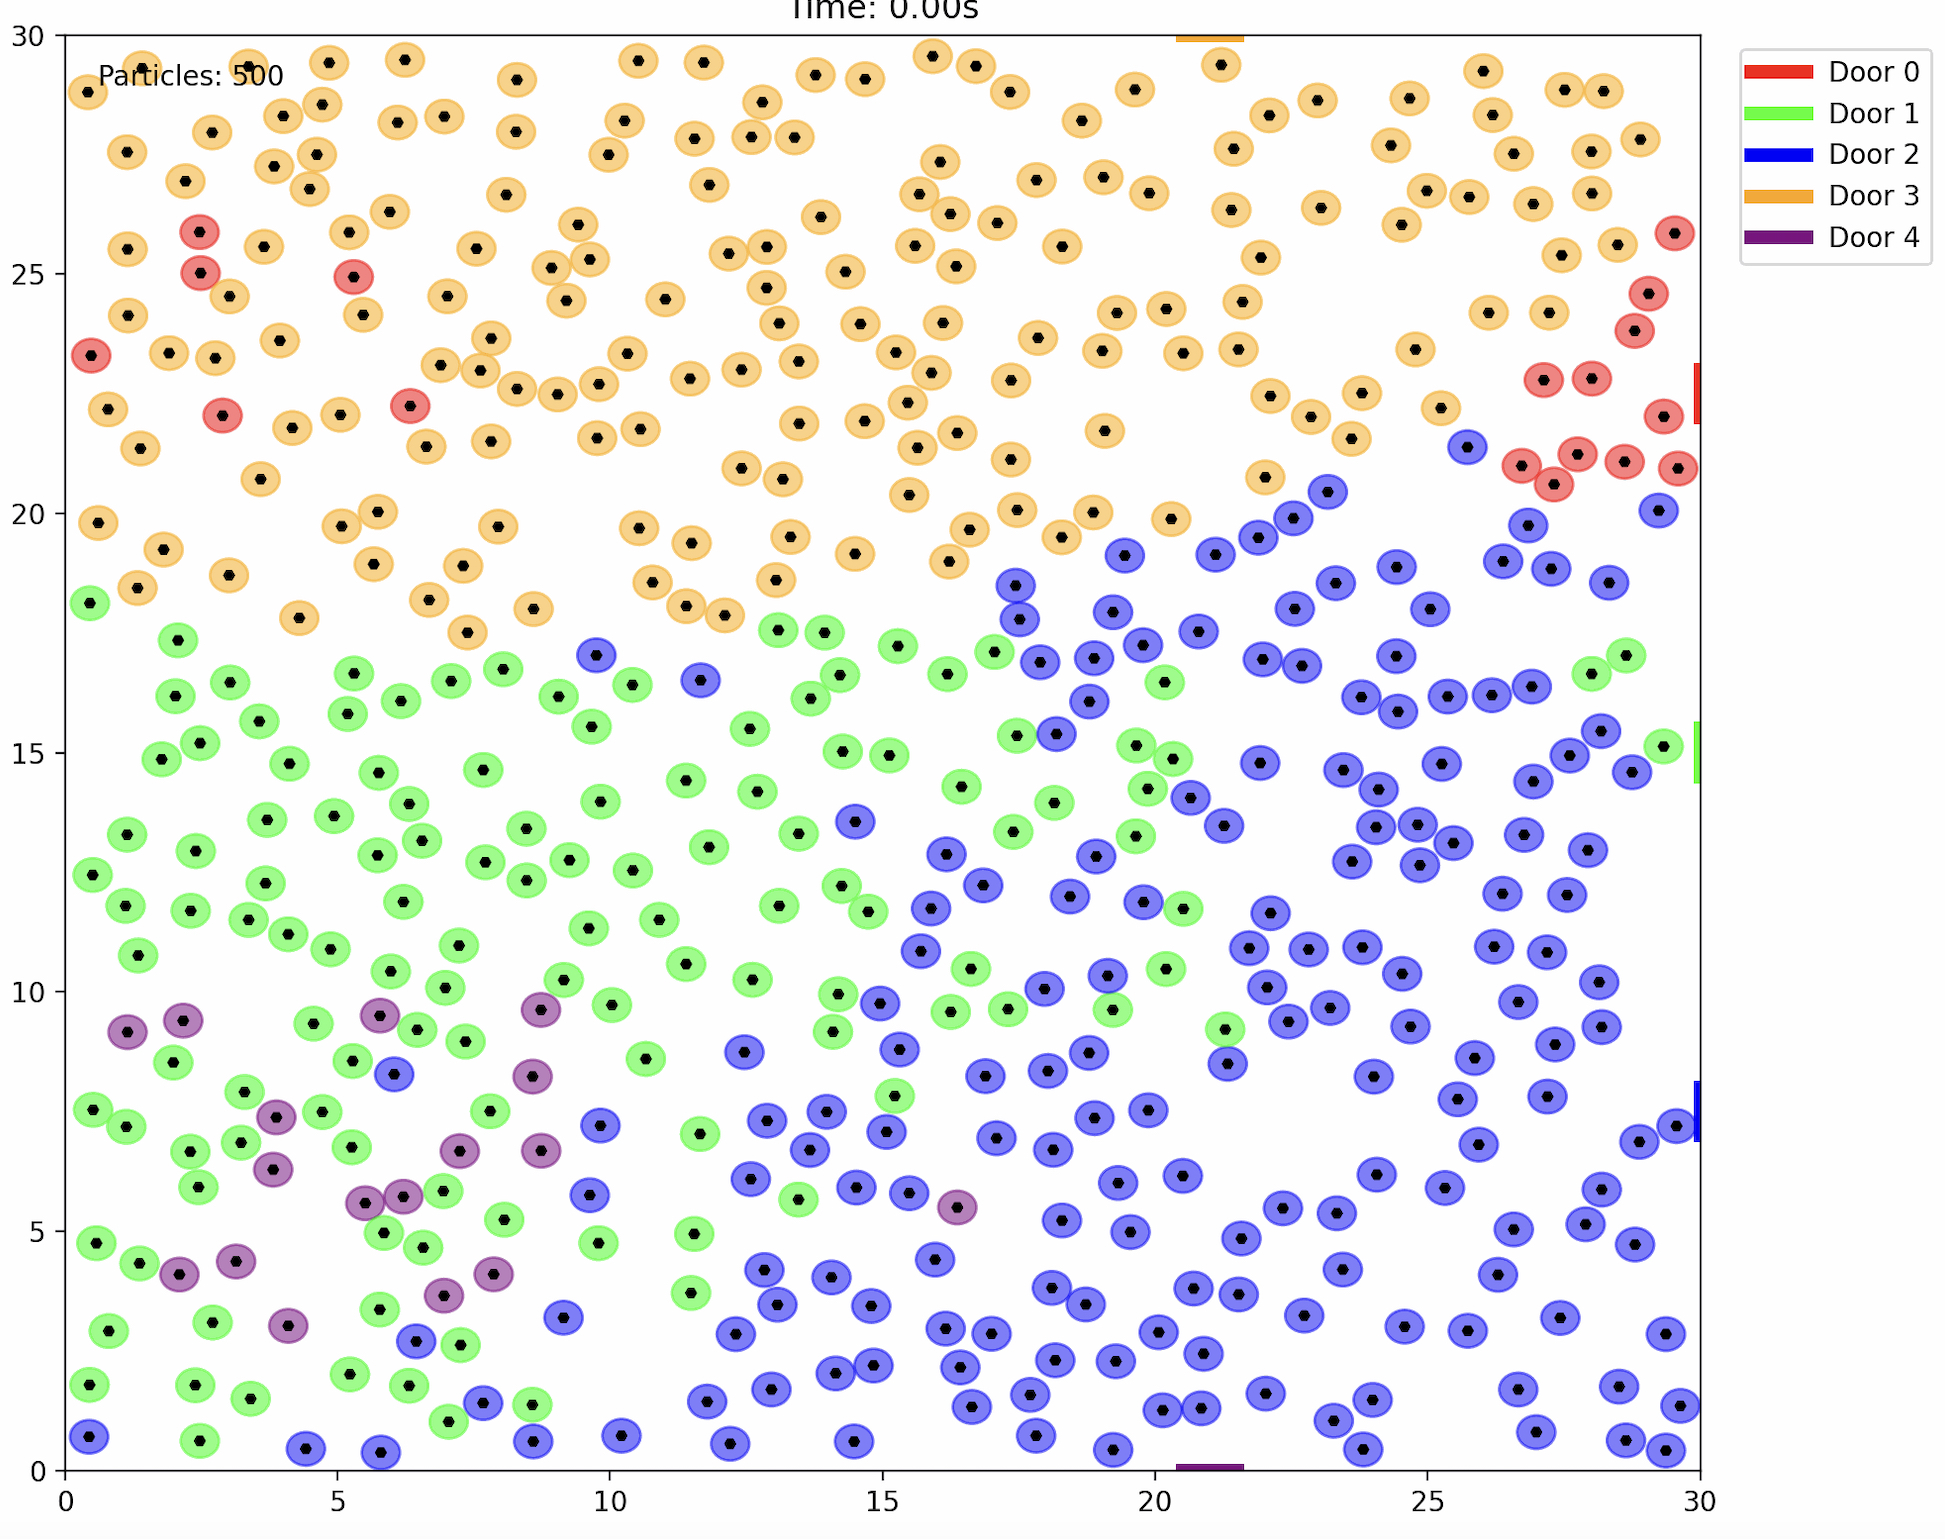
\includegraphics[width=0.4\textwidth]{img/frames/t_40_&_p_0.50.jpg}
        \caption{Diagrama UML del sistema de simulación}
    \end{figure}
\end{frame}

\begin{frame}{Contractile Particle Model}
    \begin{itemize}
        \item Autómata off-lattice
        \item Cada partícula $i$ definida por:
        \begin{itemize}
            \item Posición $\mathbf{r}_i$
            \item Radio personal variable $r_i \in [r_{\text{min}}, r_{\text{max}}]$
            \item Velocidad deseada $\mathbf{v}_d$ hacia objetivo $\mathbf{T}_i$
        \end{itemize}
    \end{itemize}
\end{frame}

\begin{frame}{Modelo}
    \begin{columns}
        \begin{column}{0.5\textwidth}
            {\centering\textbf{MOVIMIENTO}\par}
            \vspace{0.5em}
            \[
                \mathbf{r}_i(t + \Delta t) = \mathbf{r}_i(t) + \mathbf{v}_i(t)\Delta t
            \]
        \end{column}
        \begin{column}{0.5\textwidth}
            {\centering\textbf{PASO TEMPORAL}\par}
            \vspace{0.5em}
            \[
                \Delta t = \frac{r_{\text{min}}}{2v_{\text{max}}}
            \]
        \end{column}
    \end{columns}
    
    \vspace{1em}
    {\centering\textbf{RADIO}\par}
    \vspace{0.5em}
    \[
        r_i(t) = \begin{cases}
            r_{\text{min}} & \text{si hay colisión} \\
            \text{mín}(r_{\text{max}}, r_i(t - \Delta t) + \frac{r_{\text{max}}\Delta t}{\tau}) & \text{si no hay colisión}
        \end{cases}
    \]
\end{frame}

\begin{frame}{Modelo}
    \begin{columns}
        \begin{column}{0.5\textwidth}
            {\centering\textbf{MÓDULO DE LA VELOCIDAD}\par}
            \vspace{0.5em}
            \[
                v_i = v_{\text{max}}\left(\frac{r_i - r_{\text{min}}}{r_{\text{max}} - r_{\text{min}}}\right)^\beta
            \]
            \vspace{0.5em}
            \begin{itemize}
                \item $v_{\text{max}}$: Velocidad máxima de la partícula
                \item $r_i$: Radio actual de la i-ésima partícula
                \item $r_{\text{max}}$: Radio máximo de las partículas
                \item $r_{\text{min}}$: Radio mínimo de las partículas
                \item $\beta$: Coeficiente
            \end{itemize}
        \end{column}
        \begin{column}{0.5\textwidth}
            {\centering\textbf{DIRECCIÓN DE LA VELOCIDAD}\par}
            \vspace{0.5em}
            \[
                \mathbf{v}_i = \begin{cases}
                    v_i\mathbf{e}_i & \text{si no hay contacto} \\
                    v_{\text{max}}\mathbf{e}_{ij} & \text{si hay contacto}
                \end{cases}
            \]
            \vspace{0.5em}
            \begin{itemize}
                \item $\mathbf{e}_i$: Versor desde la partícula hacia el objetivo
                \item $\mathbf{e}_{ij}$: Versor desde la j-ésima partícula hacia la i-ésima partícula
            \end{itemize}
        \end{column}
    \end{columns}
\end{frame}

\begin{frame}{Heurística de Navegación}
    Score para cada puerta:
    \begin{equation}
        S(d) = p \times R_{Dist}(d) + (1-p) \times R_\rho(d)
    \end{equation}
    
    Donde:
    \begin{itemize}
        \item $S(d)$ = score de la puerta $d$
        \item $RD(d)$ = distancia relativa: $R_{Dist}(d) = 1 - \frac{Dist(d)}{\max(Dist)}$
        \item $R_\rho(d)$ = densidad relativa: $R_\rho(d) = 1 - \frac{\rho(d)}{\max(\rho)}$
    \end{itemize}
\end{frame}

\begin{frame}{Cálculo de Densidad}
    \begin{equation}
        \rho(d) = \frac{k}{\pi r_k^2/2}
    \end{equation}
    
    Donde:
    \begin{itemize}
        \item $k=5$ partículas más cercanas
        \item $r_k$ = distancia hasta la quinta partícula
        \item Se mide desde el centro de cada puerta
    \end{itemize}
\end{frame}
\section{Implementación}

\begin{frame}{Diagrama UML}
    \begin{figure}
        \centering
        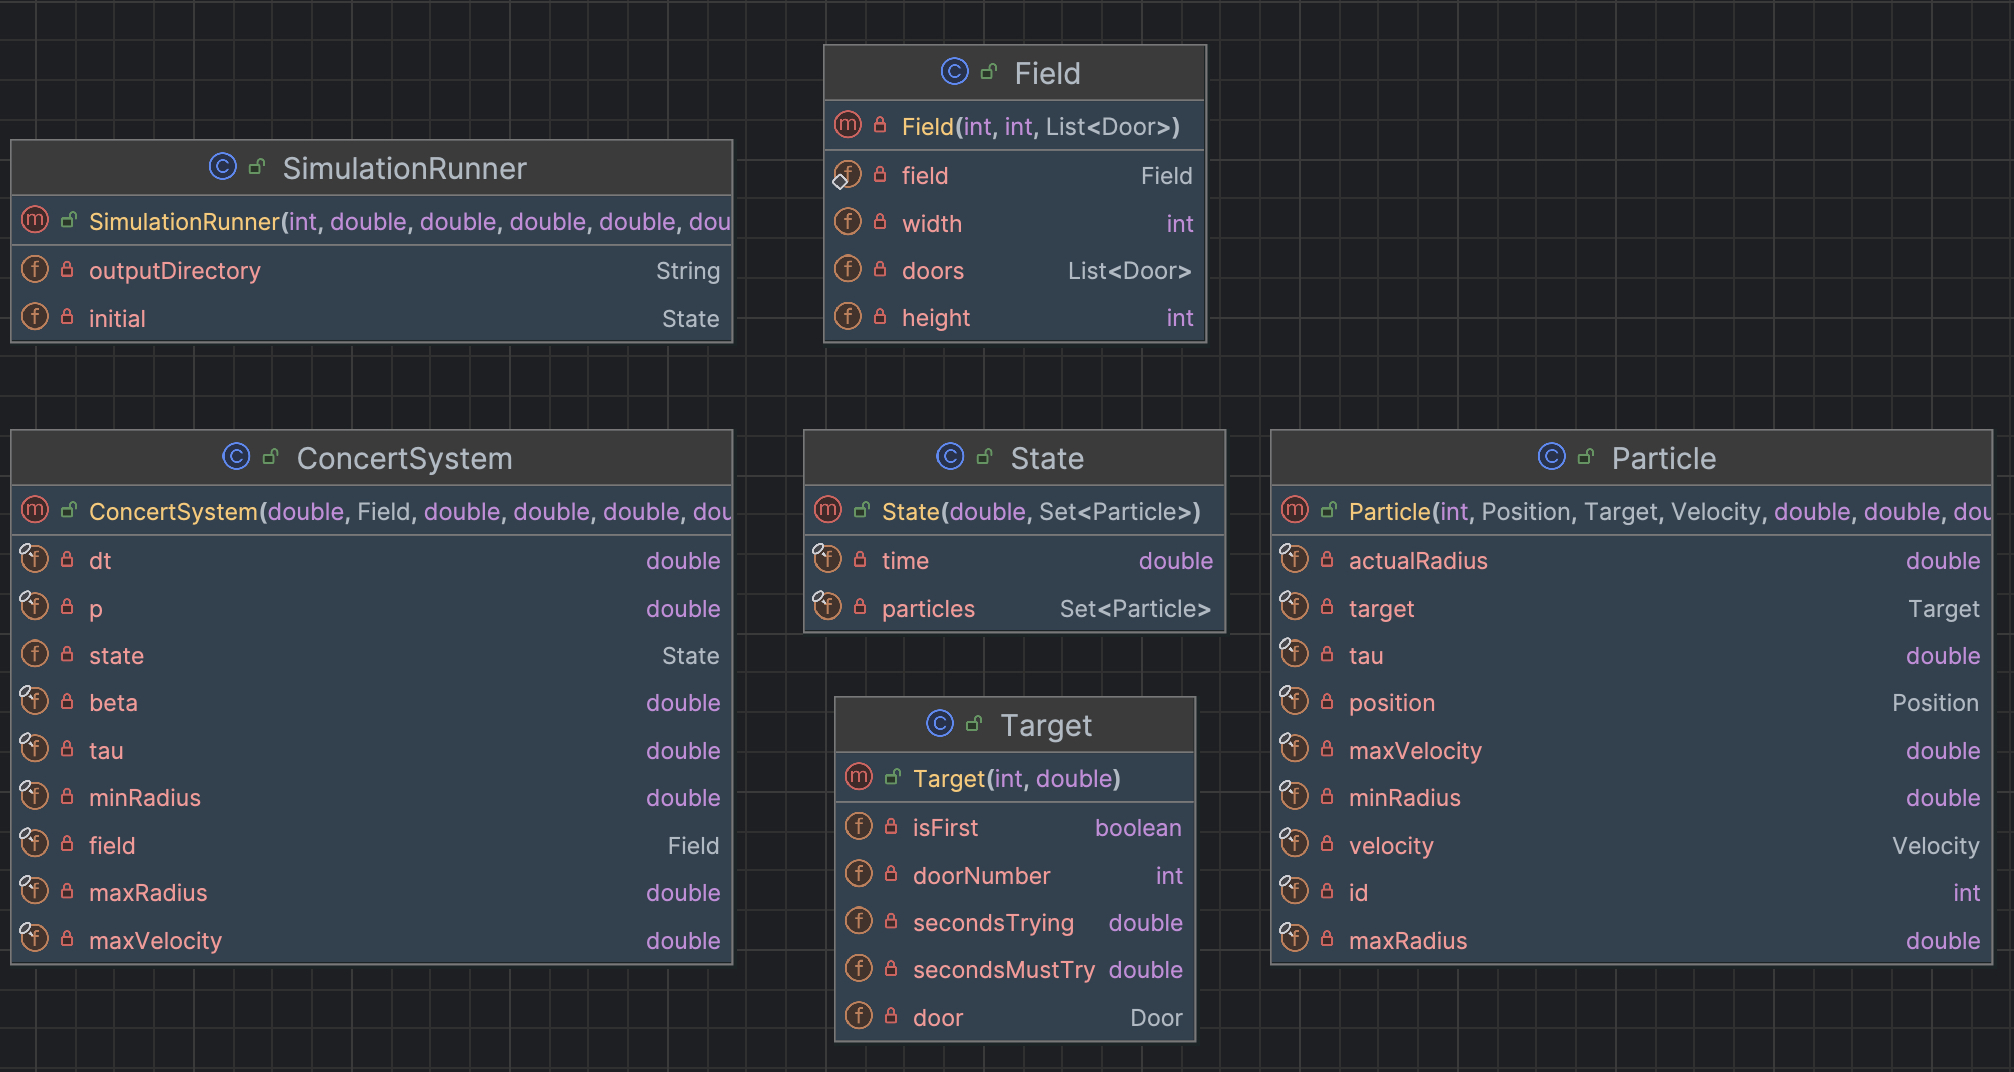
\includegraphics[width=0.8\textwidth]{img/UML.jpg}
        \caption{Diagrama UML del sistema de simulación}
    \end{figure}
\end{frame}

\begin{frame}{Evolución Temporal}
    \begin{algorithm}[H]
        \begin{algorithmic}[1]
            \State $\texttt{newParticles} \leftarrow \emptyset$
            \For{$p \in \texttt{state.getParticles()}$}
                \State $\texttt{newParticle} \leftarrow \texttt{escape}(p)$
                \If{$\neg \texttt{hasEscaped}(\texttt{newParticle})$}
                    \State $\texttt{newParticles} \leftarrow \texttt{newParticles} \cup \{\texttt{newParticle}\}$
                \EndIf
            \EndFor
            \State \Return $\texttt{new State}(\texttt{time} + \Delta t, \texttt{newParticles})$
        \end{algorithmic}
    \end{algorithm}
\end{frame}

\begin{frame}{Mecanismo de Escape}
    \begin{algorithm}[H]
        \begin{algorithmic}[1]
            \Function{escape}{$p$}
                \State $\texttt{contacts} \leftarrow \texttt{checkContact}(p)$
                \State $\texttt{newRadius} \leftarrow \texttt{updateRadius}(p, \neg \texttt{contacts.isEmpty()})$
                \State $\texttt{newModule} \leftarrow \texttt{updateModule}(p, \texttt{newRadius})$
                \State $\texttt{newDirection} \leftarrow \texttt{updateDirection}(p, \texttt{contacts})$
                \State $\texttt{newPosition} \leftarrow \texttt{updatePosition}(p, \Delta t)$
                \State $p.\texttt{target.step}(\Delta t)$
                \If{$p.\texttt{target.needsChange()}$}
                    \State $p.\texttt{target.change}(\texttt{bestNextDoor}(p))$
                \EndIf
                \State \Return nueva Partícula$(p.\texttt{id}, \texttt{newPosition}, p.\texttt{target}, \texttt{newDirection}, \texttt{newModule})$
            \EndFunction
        \end{algorithmic}
    \end{algorithm}
\end{frame}

\section{Simulaciones}

\begin{frame}{Parámetros y variables}
    \begin{columns}
        \begin{column}{0.5\textwidth}
            {\centering\textbf{VARIABLES}\par}
            \vspace{0.5em}
            \begin{itemize}
                \item Factor $p$: Balance entre distancia y densidad
                \item Tiempo de re-decisión $ct$: Intervalo de re-evaluación
            \end{itemize}
        \end{column}
        \begin{column}{0.5\textwidth}
            {\centering\textbf{PARÁMETROS}\par}
            \vspace{0.5em}
            \begin{align*}
                r_{\text{min}} &= 0.15\text{ m} \\
                r_{\text{max}} &= 0.35\text{ m} \\
                v_{\text{max}} &= 1.0\text{ m/s} \\
                N_{\text{agentes}} &= 500 \\
                \beta &= 0.9 \\
                \tau &= 0.5\text{ s}
            \end{align*}
        \end{column}
    \end{columns}
\end{frame}

\begin{frame}{Observable: Tiempo de Evacuación}
    \begin{itemize}
        \item Medición del tiempo total hasta evacuación completa
        \item Análisis de dependencia con parámetros:
        \begin{itemize}
            \item Variación con tiempo de re-decisión
            \item Impacto del factor de ponderación $p$
        \end{itemize}
    \end{itemize}
\end{frame}

\begin{frame}{Observable: Cálculo del Caudal}
    \begin{itemize}
        \item Caudal total:
        \begin{equation}
            Q(t) = N(t) - N(t + \Delta t)
        \end{equation}
        \item Métricas analizadas:
        \begin{itemize}
            \item $Q_{global}$: agentes por puerta / tiempo total
            \item Interpolación lineal de curvas $N(t)$
        \end{itemize}
    \end{itemize}
\end{frame}

\begin{frame}{Observable: Densidad Media}
    \begin{equation}
        \rho(t) = \frac{1}{N} \sum_{i=1}^{N} \frac{n_i(t)}{A_c}
    \end{equation}
    
    Donde:
    \begin{itemize}
        \item $N$ = número total de circunferencias
        \item $n_i(t)$ = partículas en circunferencia $i$ en tiempo $t$
        \item $A_c$ = área de cada (semi) circunferencia
    \end{itemize}
\end{frame}

\begin{frame}{Observable: Coeficiente de Uniformidad}
    \begin{itemize}
        \item Definiciones:
        \begin{itemize}
            \item $n_i(t)$ = partículas que salieron por puerta $i$ hasta tiempo $t$
            \item $\Delta n_i(t) = n_i(t + \Delta t) - n_i(t)$
        \end{itemize}
        \item Coeficiente:
        \begin{equation}
            U(t) = 1 - \frac{\sigma(t)}{\mu(t)}
        \end{equation}
    \end{itemize}
\end{frame}


\section{Resultados}

\begin{frame}{Análisis del tiempo de evacuación en función de $p$, con $ct=45$}
    \begin{figure}
        \centering
        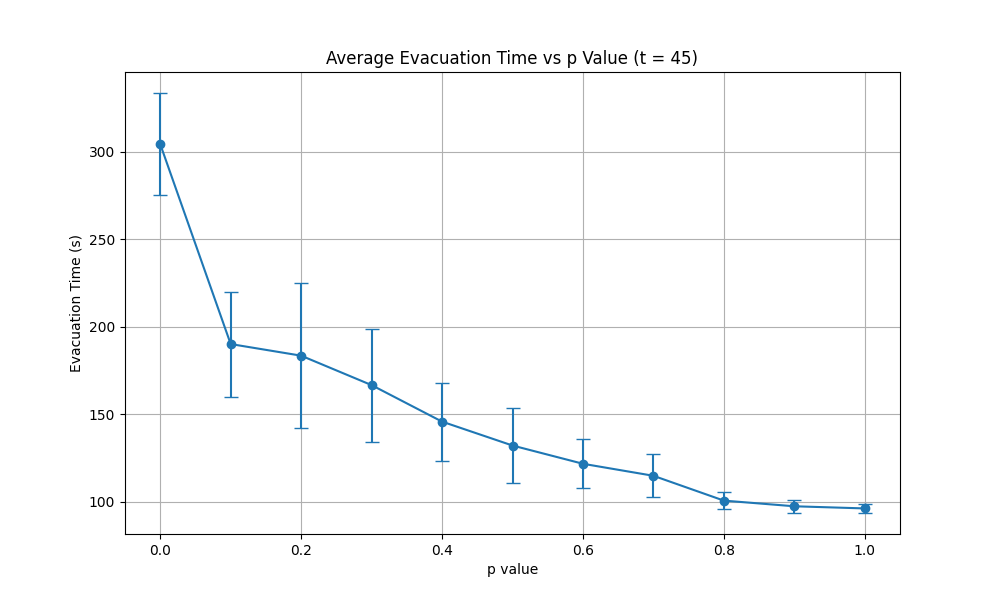
\includegraphics[width=0.60\textwidth]{img/evacuation_times_t_45.png}
        \caption{Tiempo promedio de evacuación en función del parámetro de ponderación ($p$) para $ct=45$}
    \end{figure}
\end{frame}

\begin{frame}{Flujo Acumulado ($p=1.00$): Priorizando la Distancia}
    \begin{figure}
        \centering
        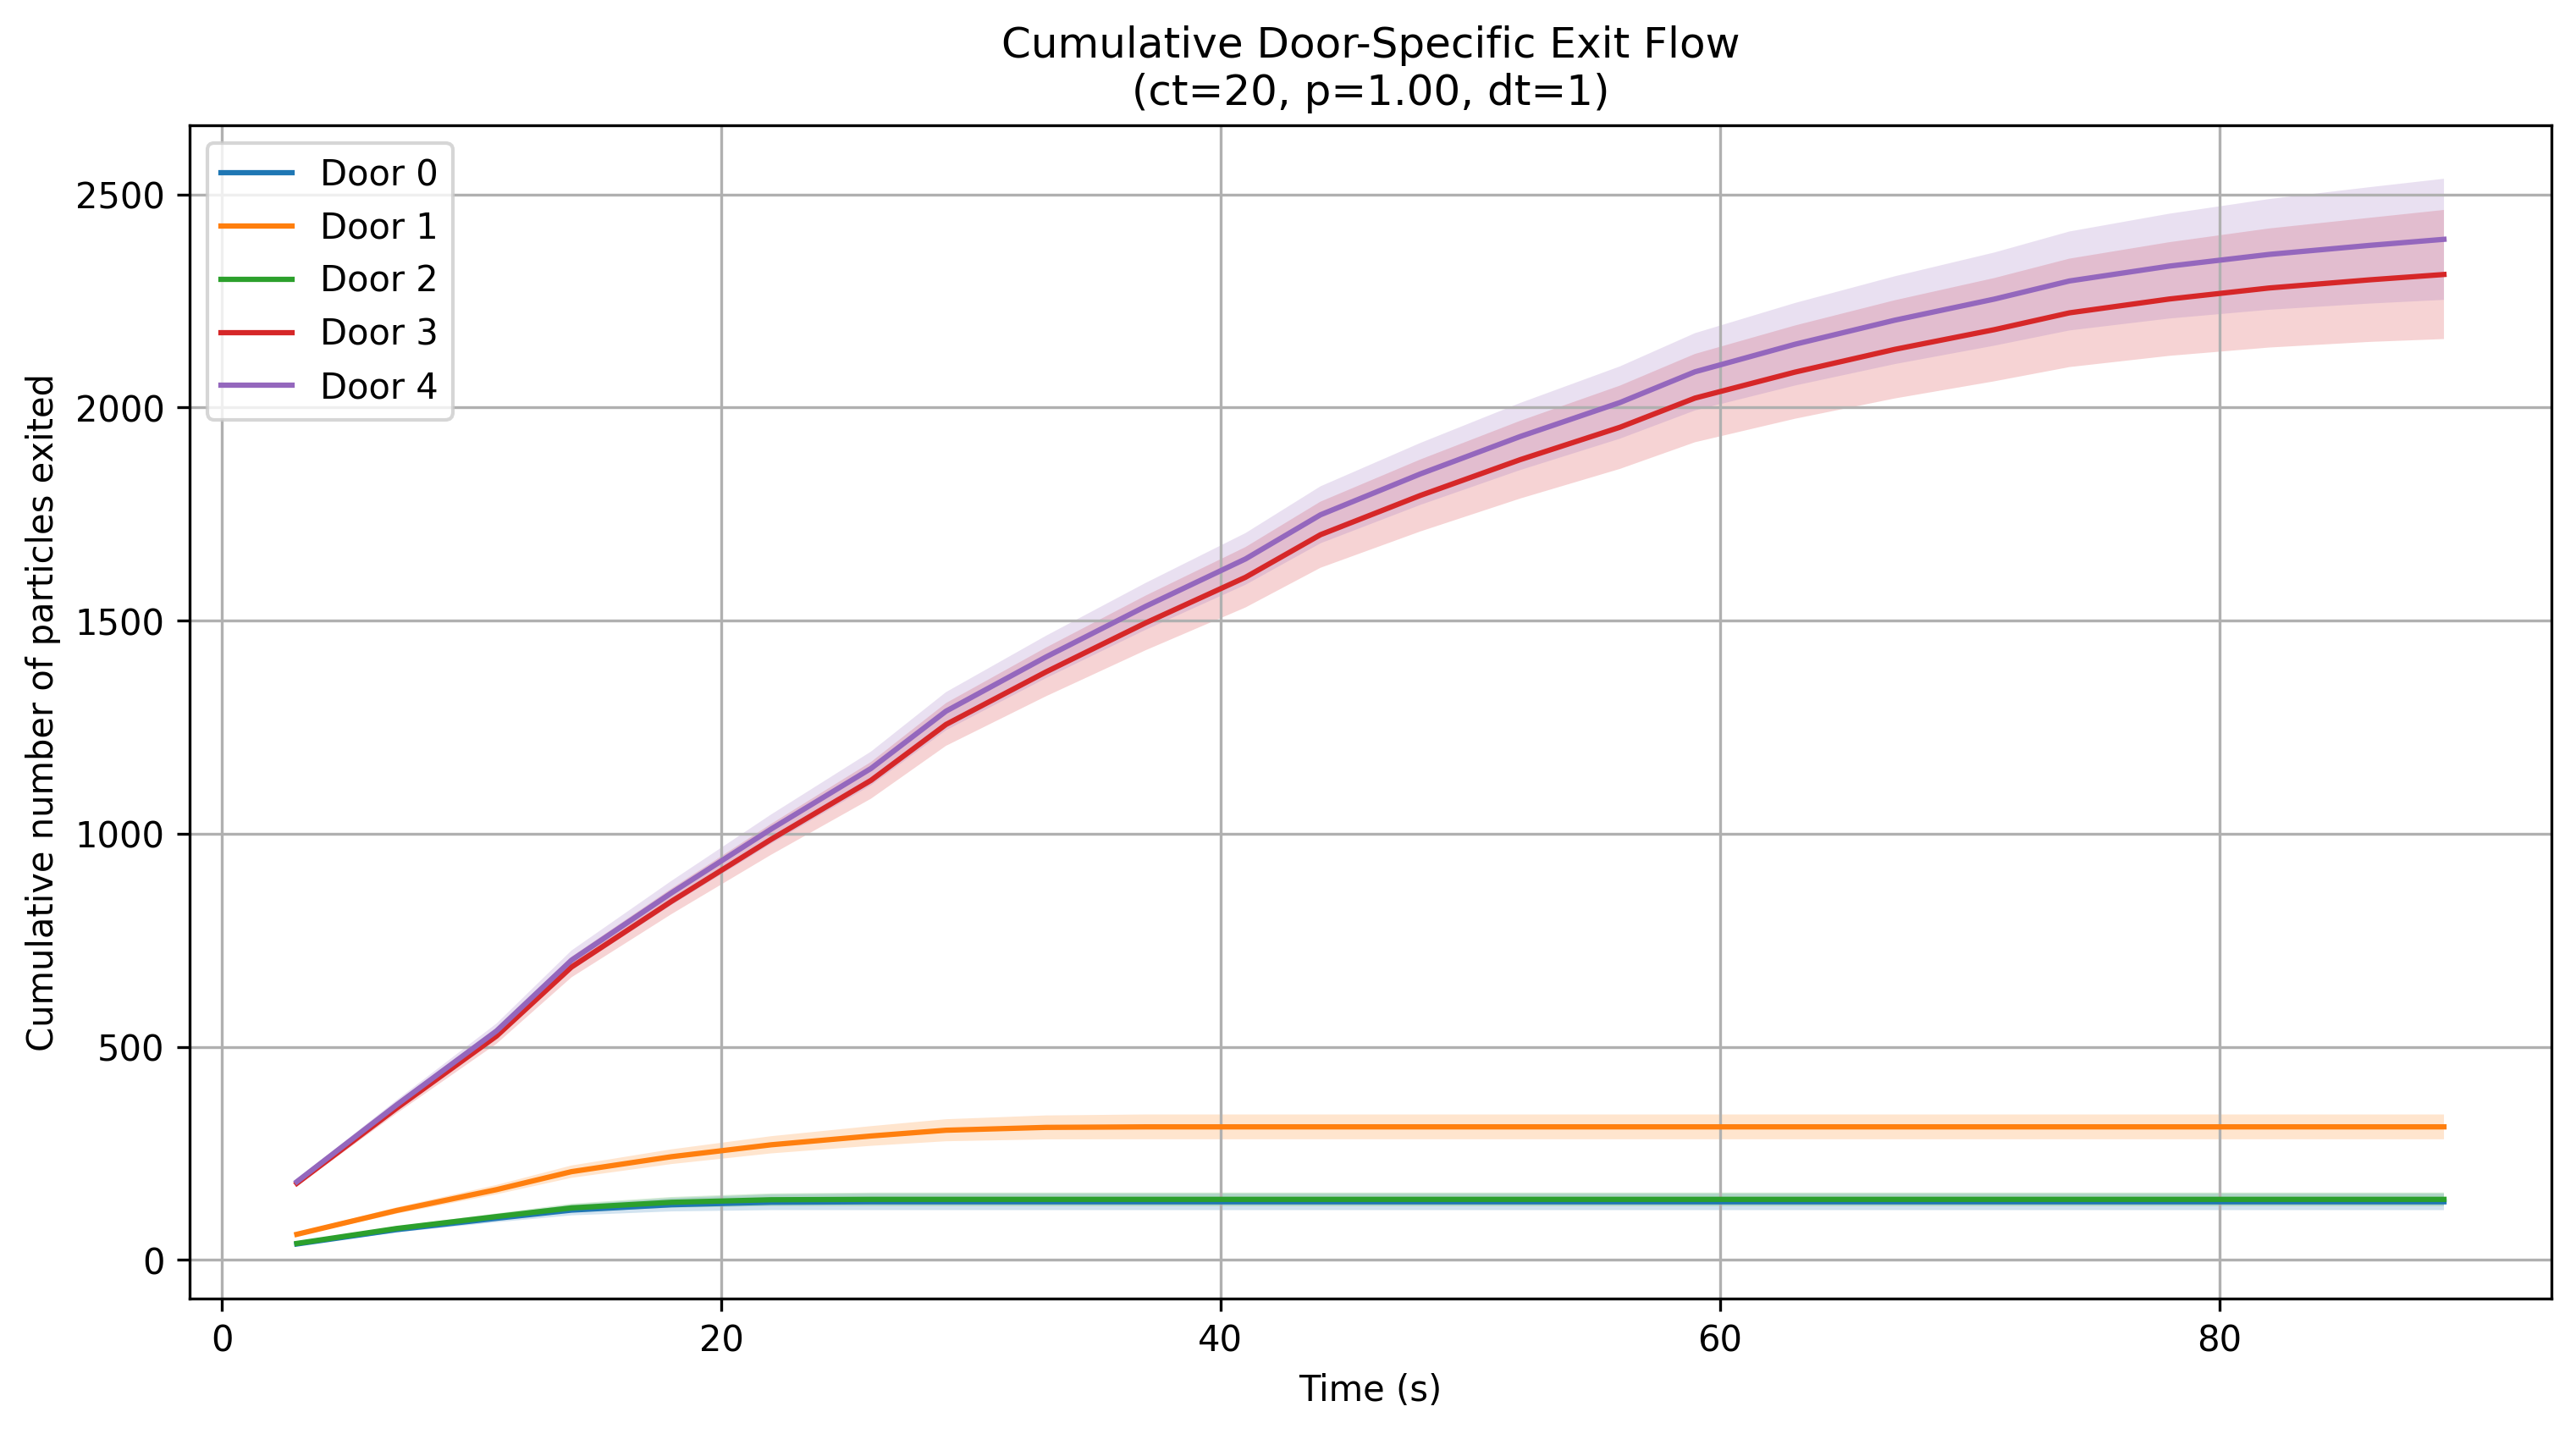
\includegraphics[width=0.6\textwidth]{img/cumulative_door_flows_t_20_&_p_1.00.png}
        \caption{Flujo acumulado de evacuación para $p=1.00$}
    \end{figure}
\end{frame}

\begin{frame}{Flujo Acumulado ($p=0.50$)}
    \begin{figure}
        \centering
        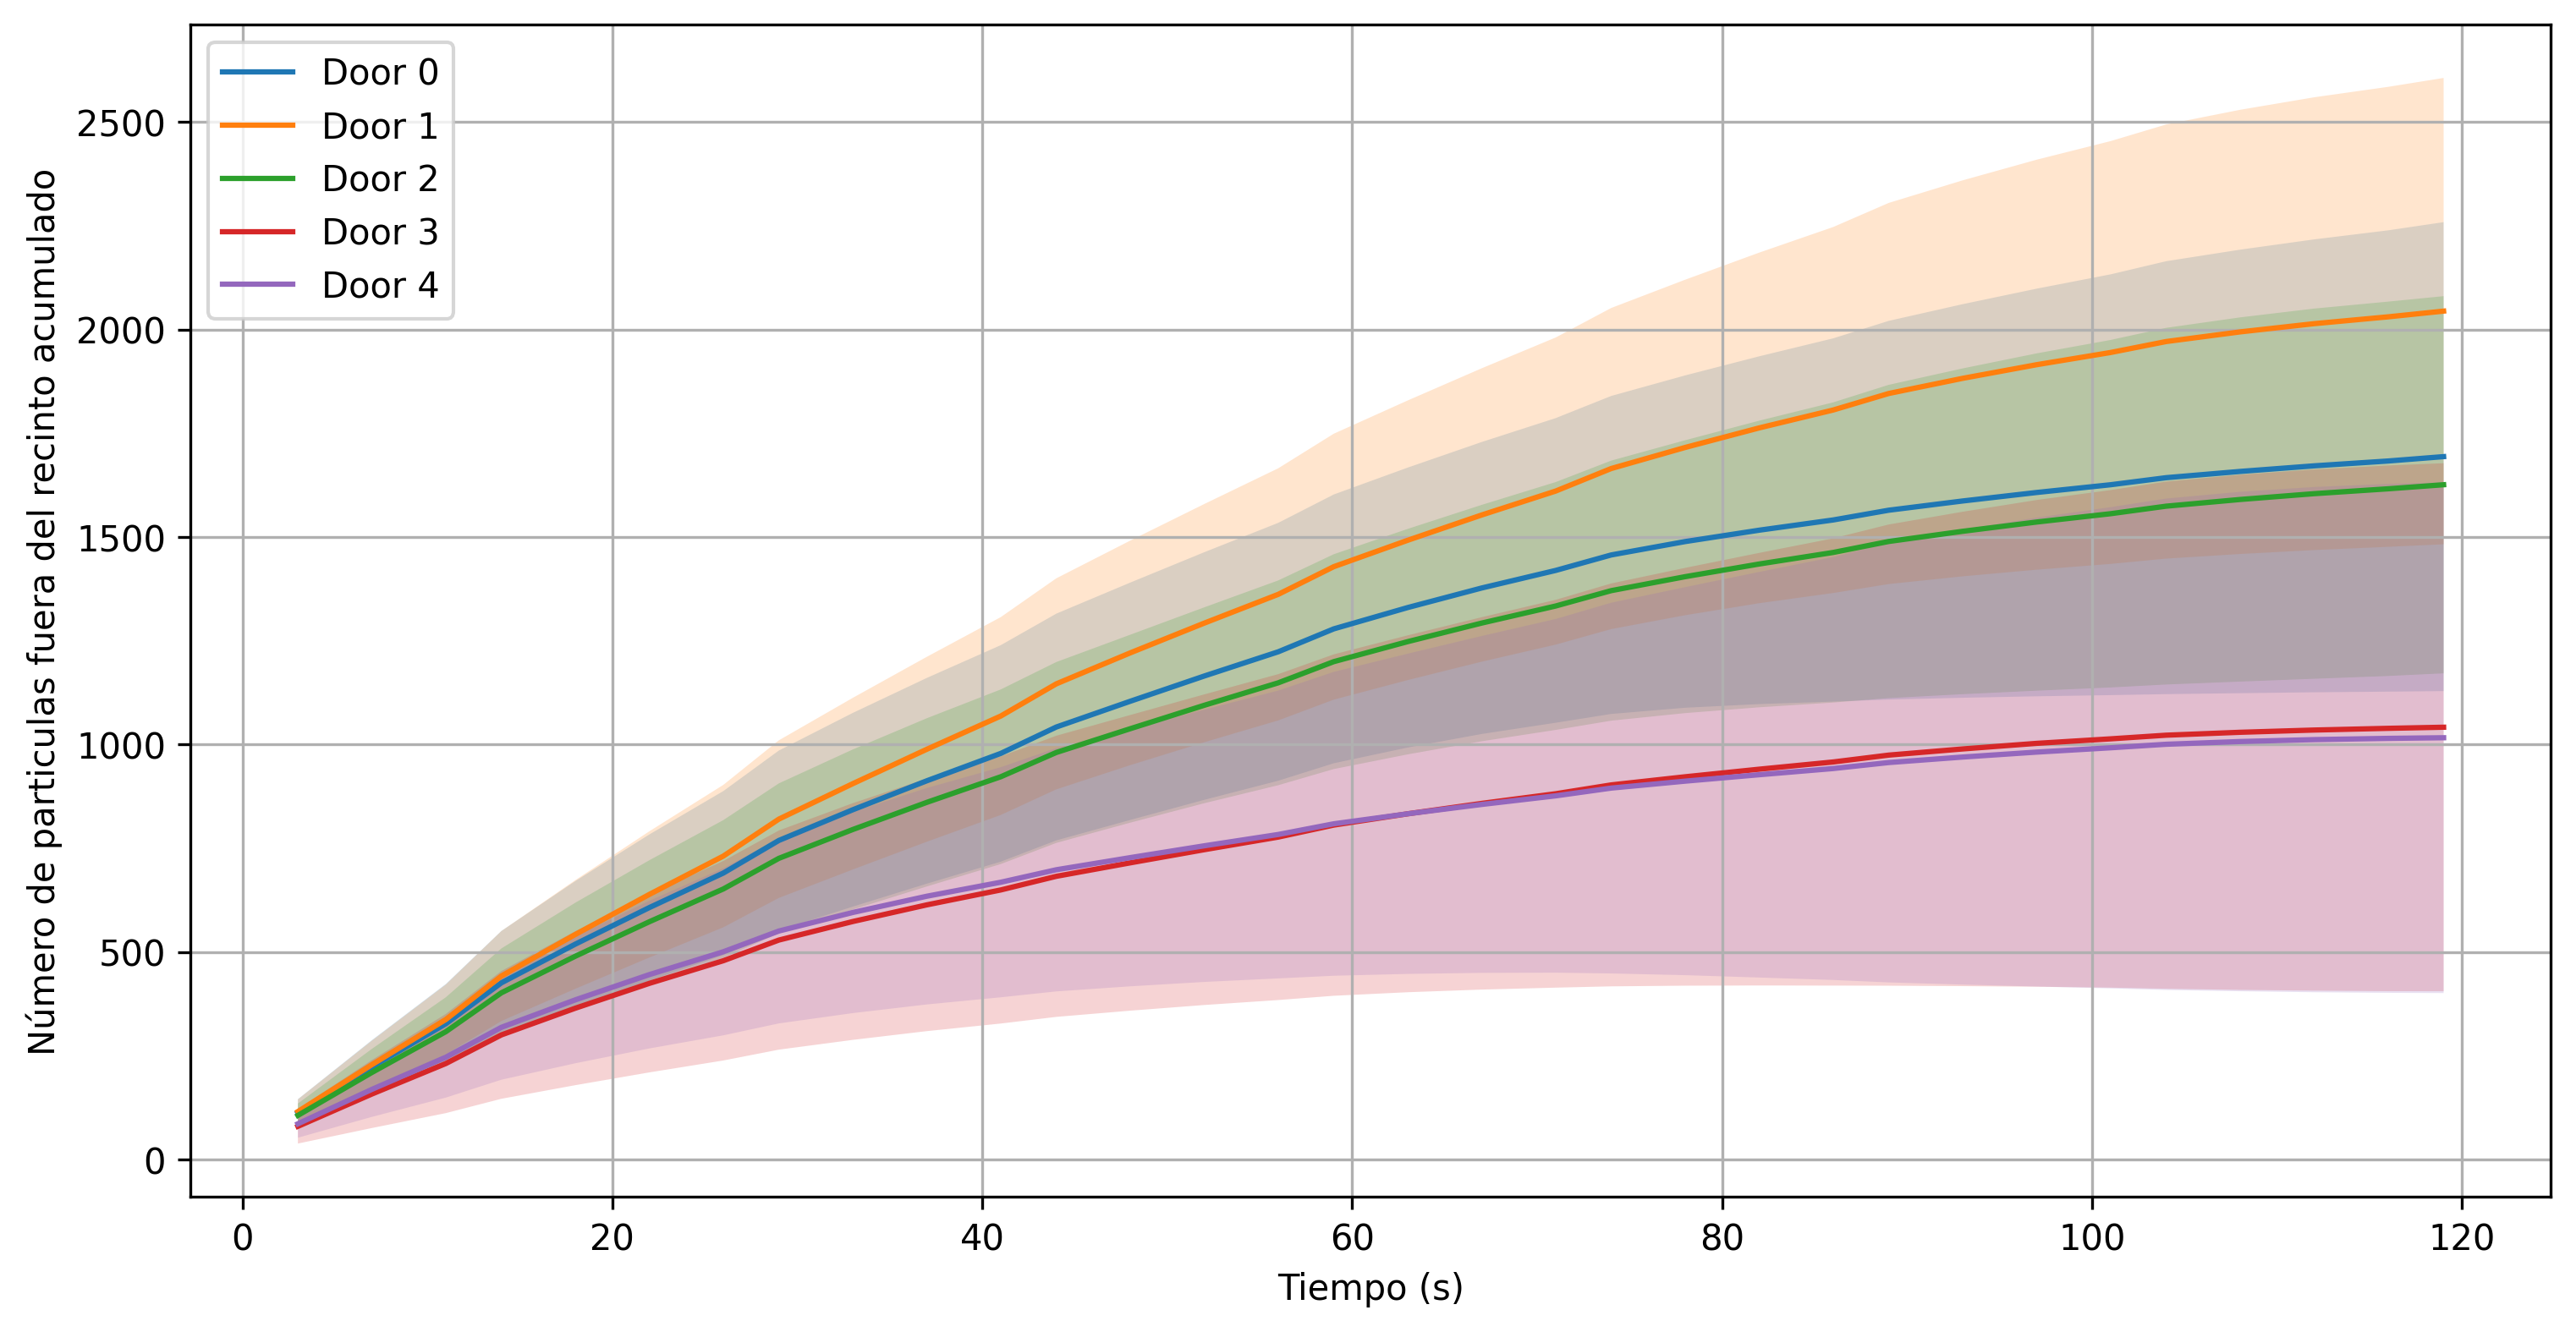
\includegraphics[width=0.6\textwidth]{img/cumulative_door_flows_t_20_&_p_0.50.png}
        \caption{Flujo acumulado de evacuación para $p=0.50$}
    \end{figure}
\end{frame}

\begin{frame}{Flujo Acumulado ($p=0.00$)}
    \begin{figure}
        \centering
        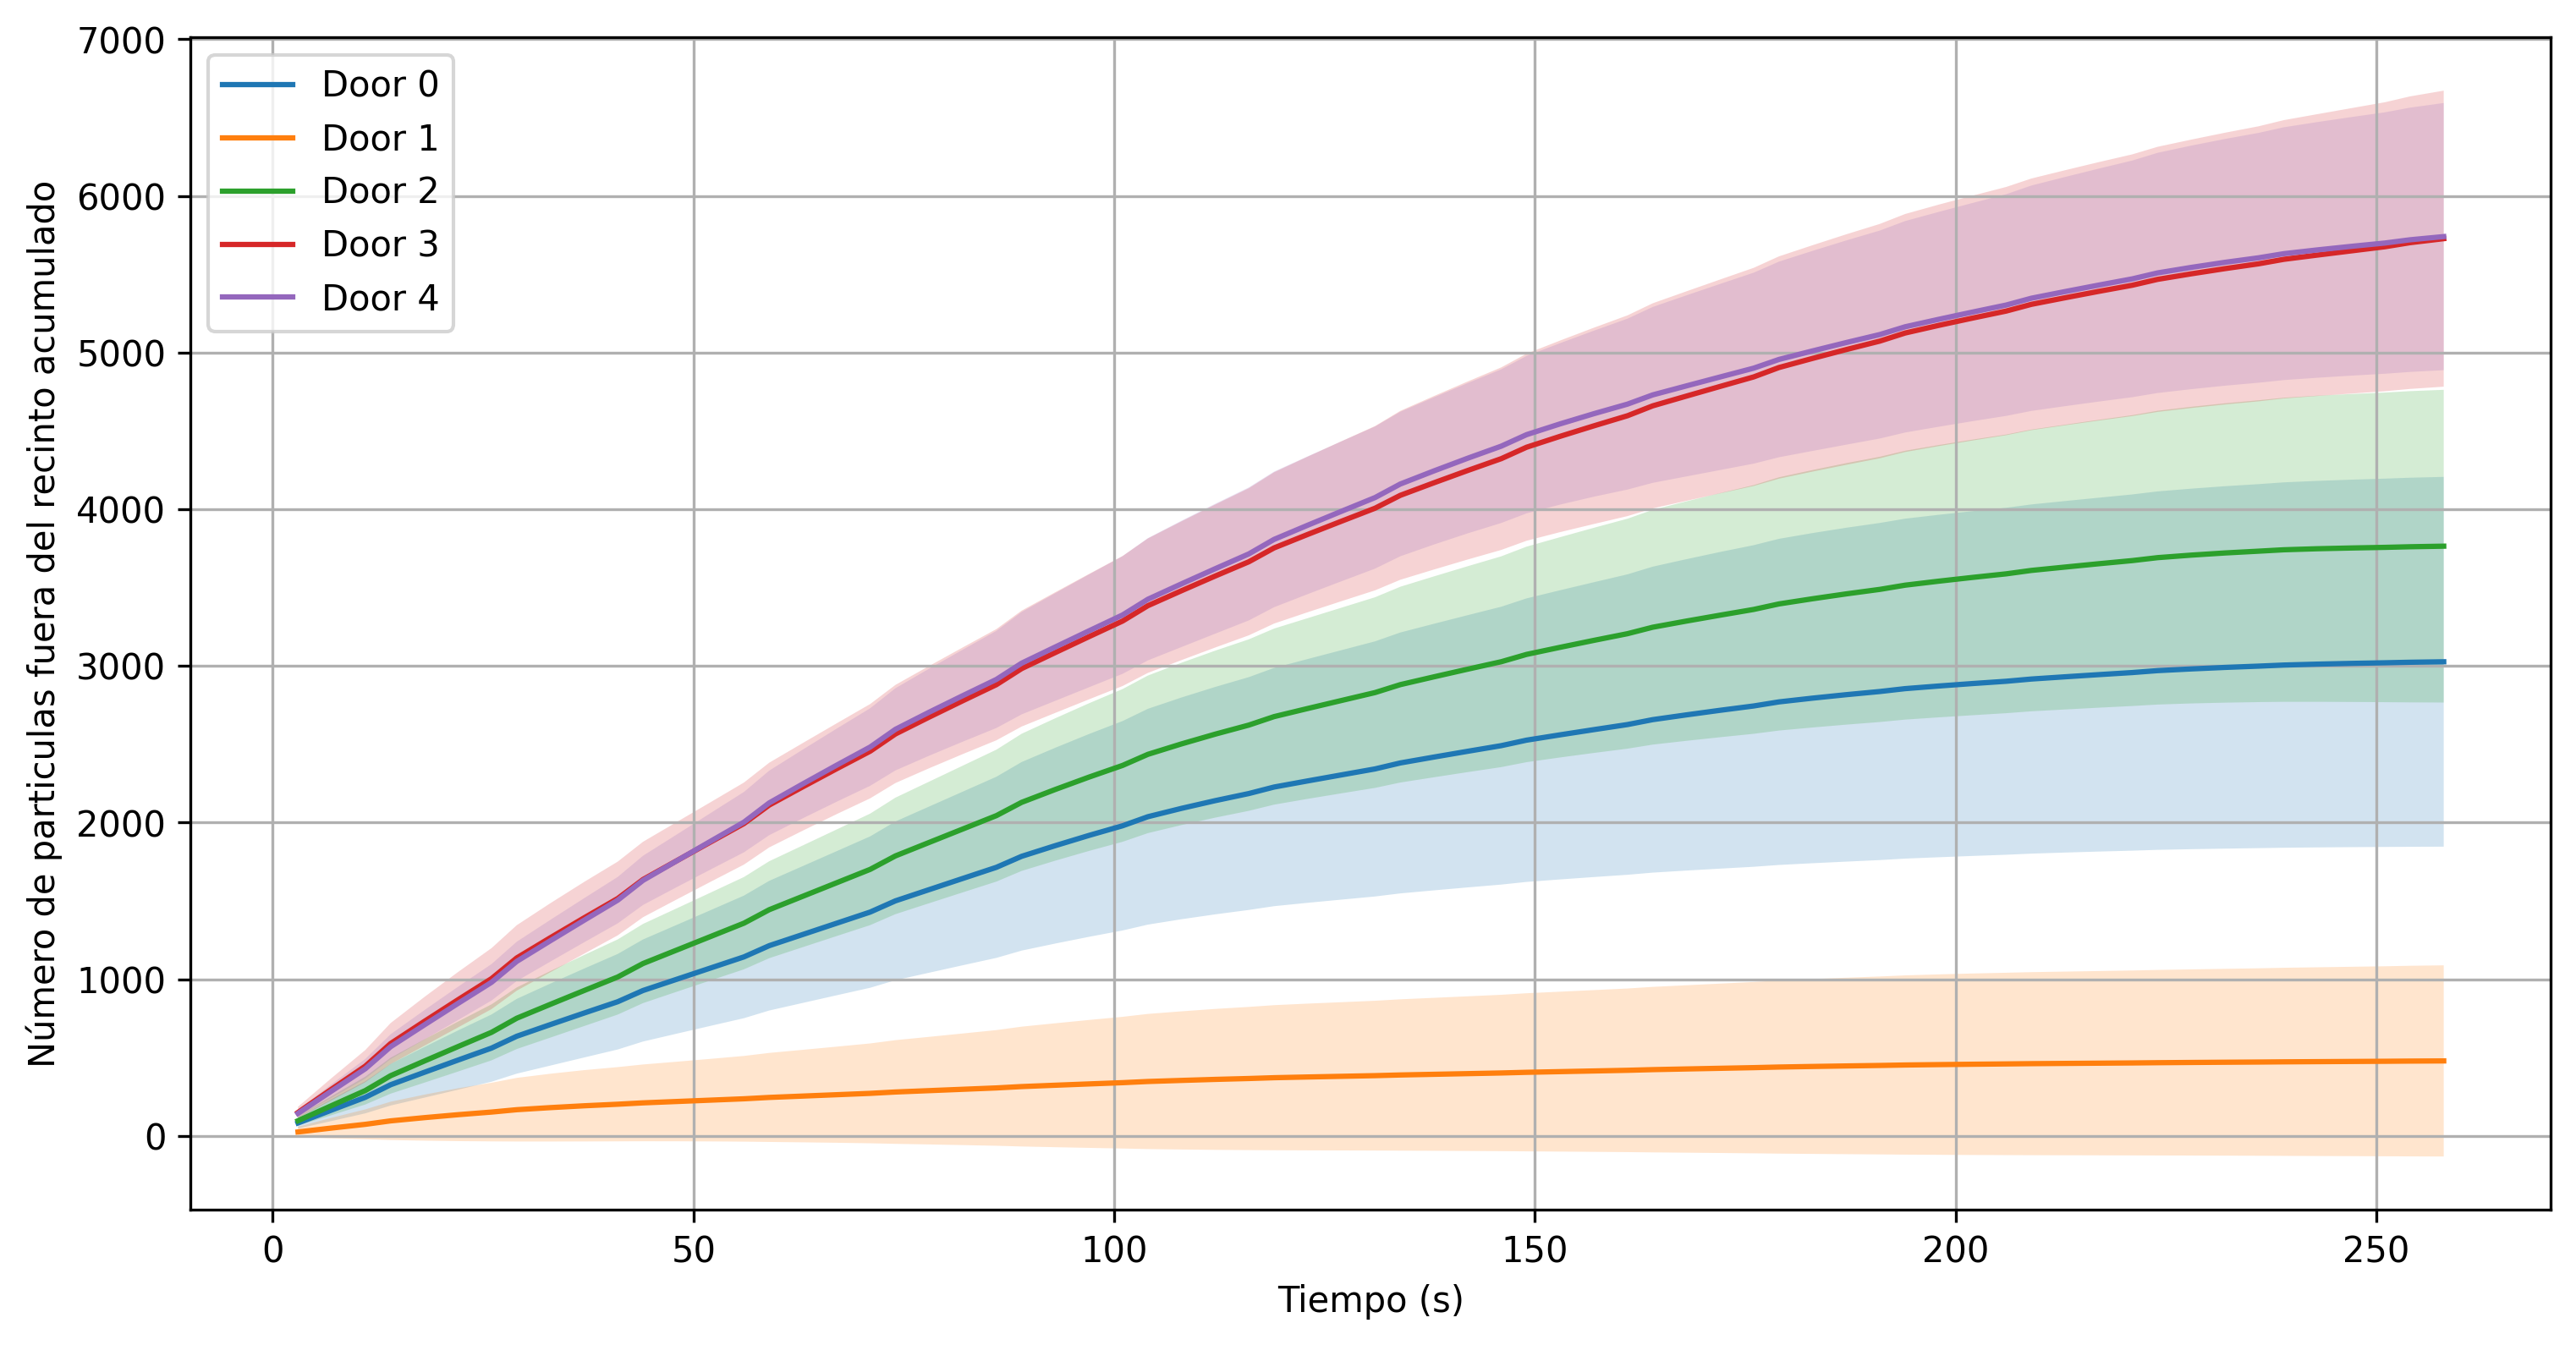
\includegraphics[width=0.6\textwidth]{img/cumulative_door_flows_t_20_&_p_0.00.png}
        \caption{Flujo acumulado de evacuación para $p=0.00$}
    \end{figure}
\end{frame}

\begin{frame}{Caudal Global}
    \begin{figure}
        \centering
        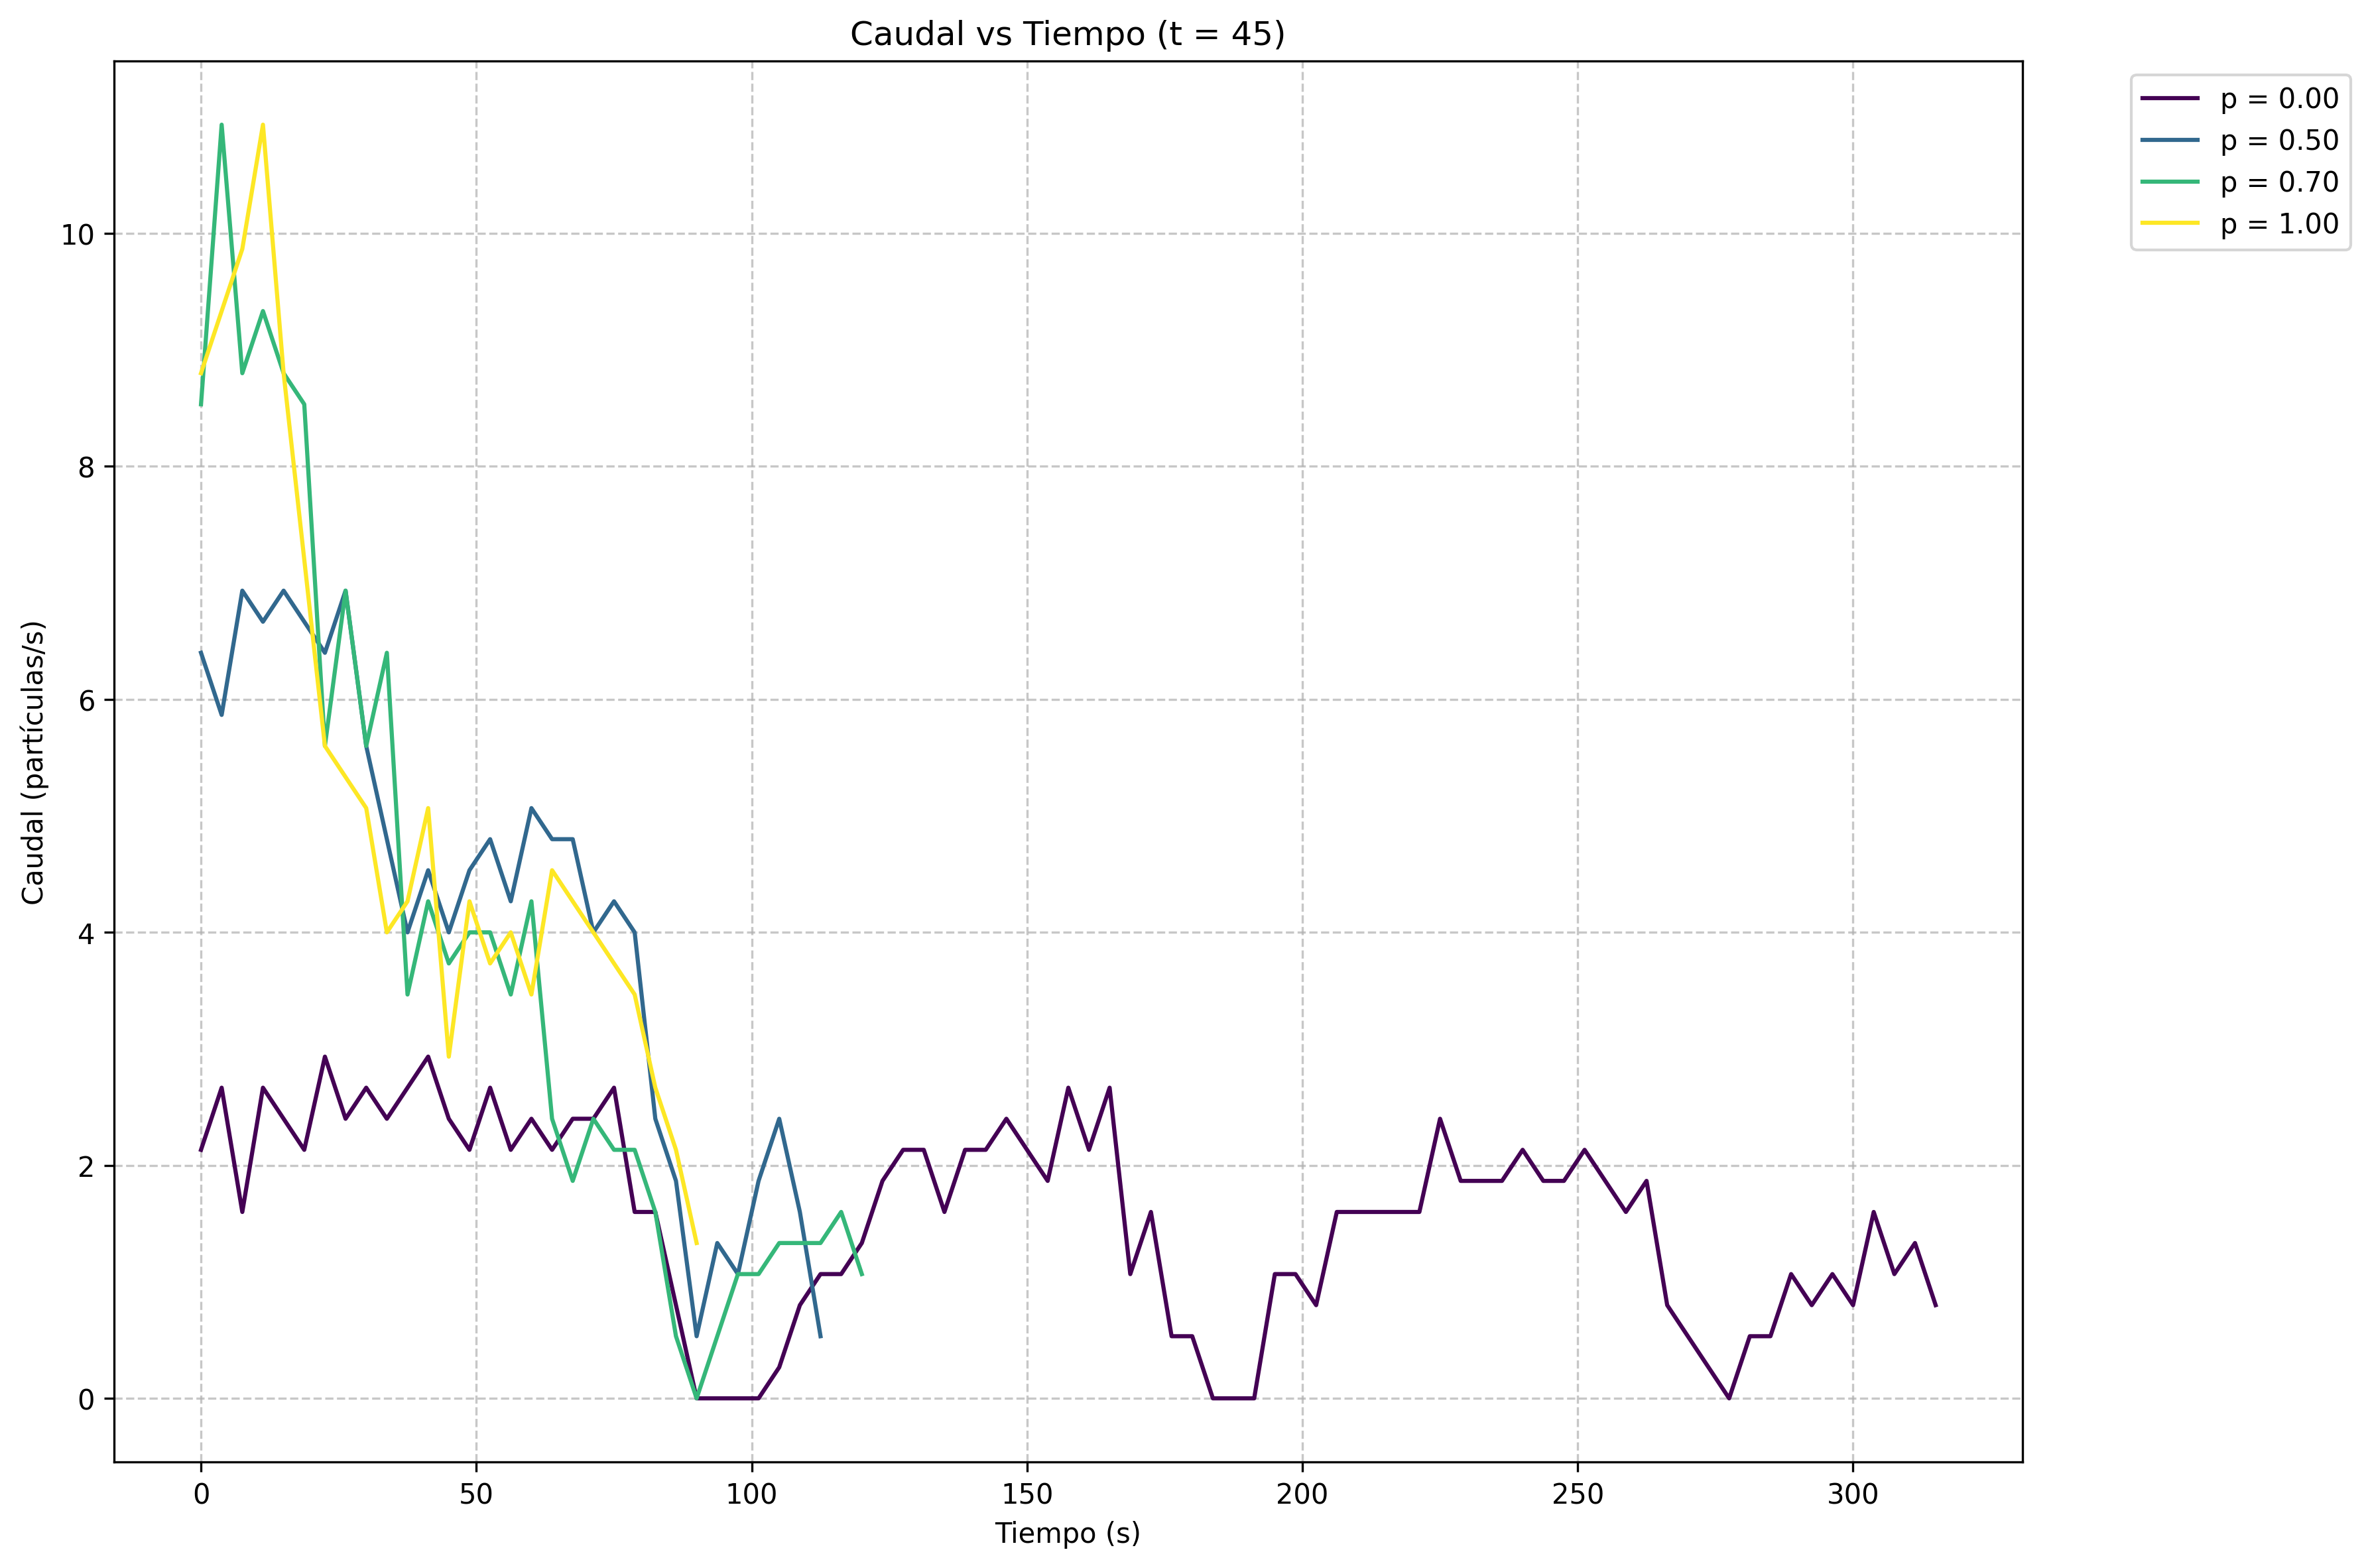
\includegraphics[width=0.6\textwidth]{img/caudal_vs_time_t45.png}
        \caption{Caudal global en función del tiempo ($ct=45$)}
    \end{figure}
\end{frame}

\begin{frame}{Caudal por Puerta ($p=1.00$)}
    \begin{figure}
        \centering
        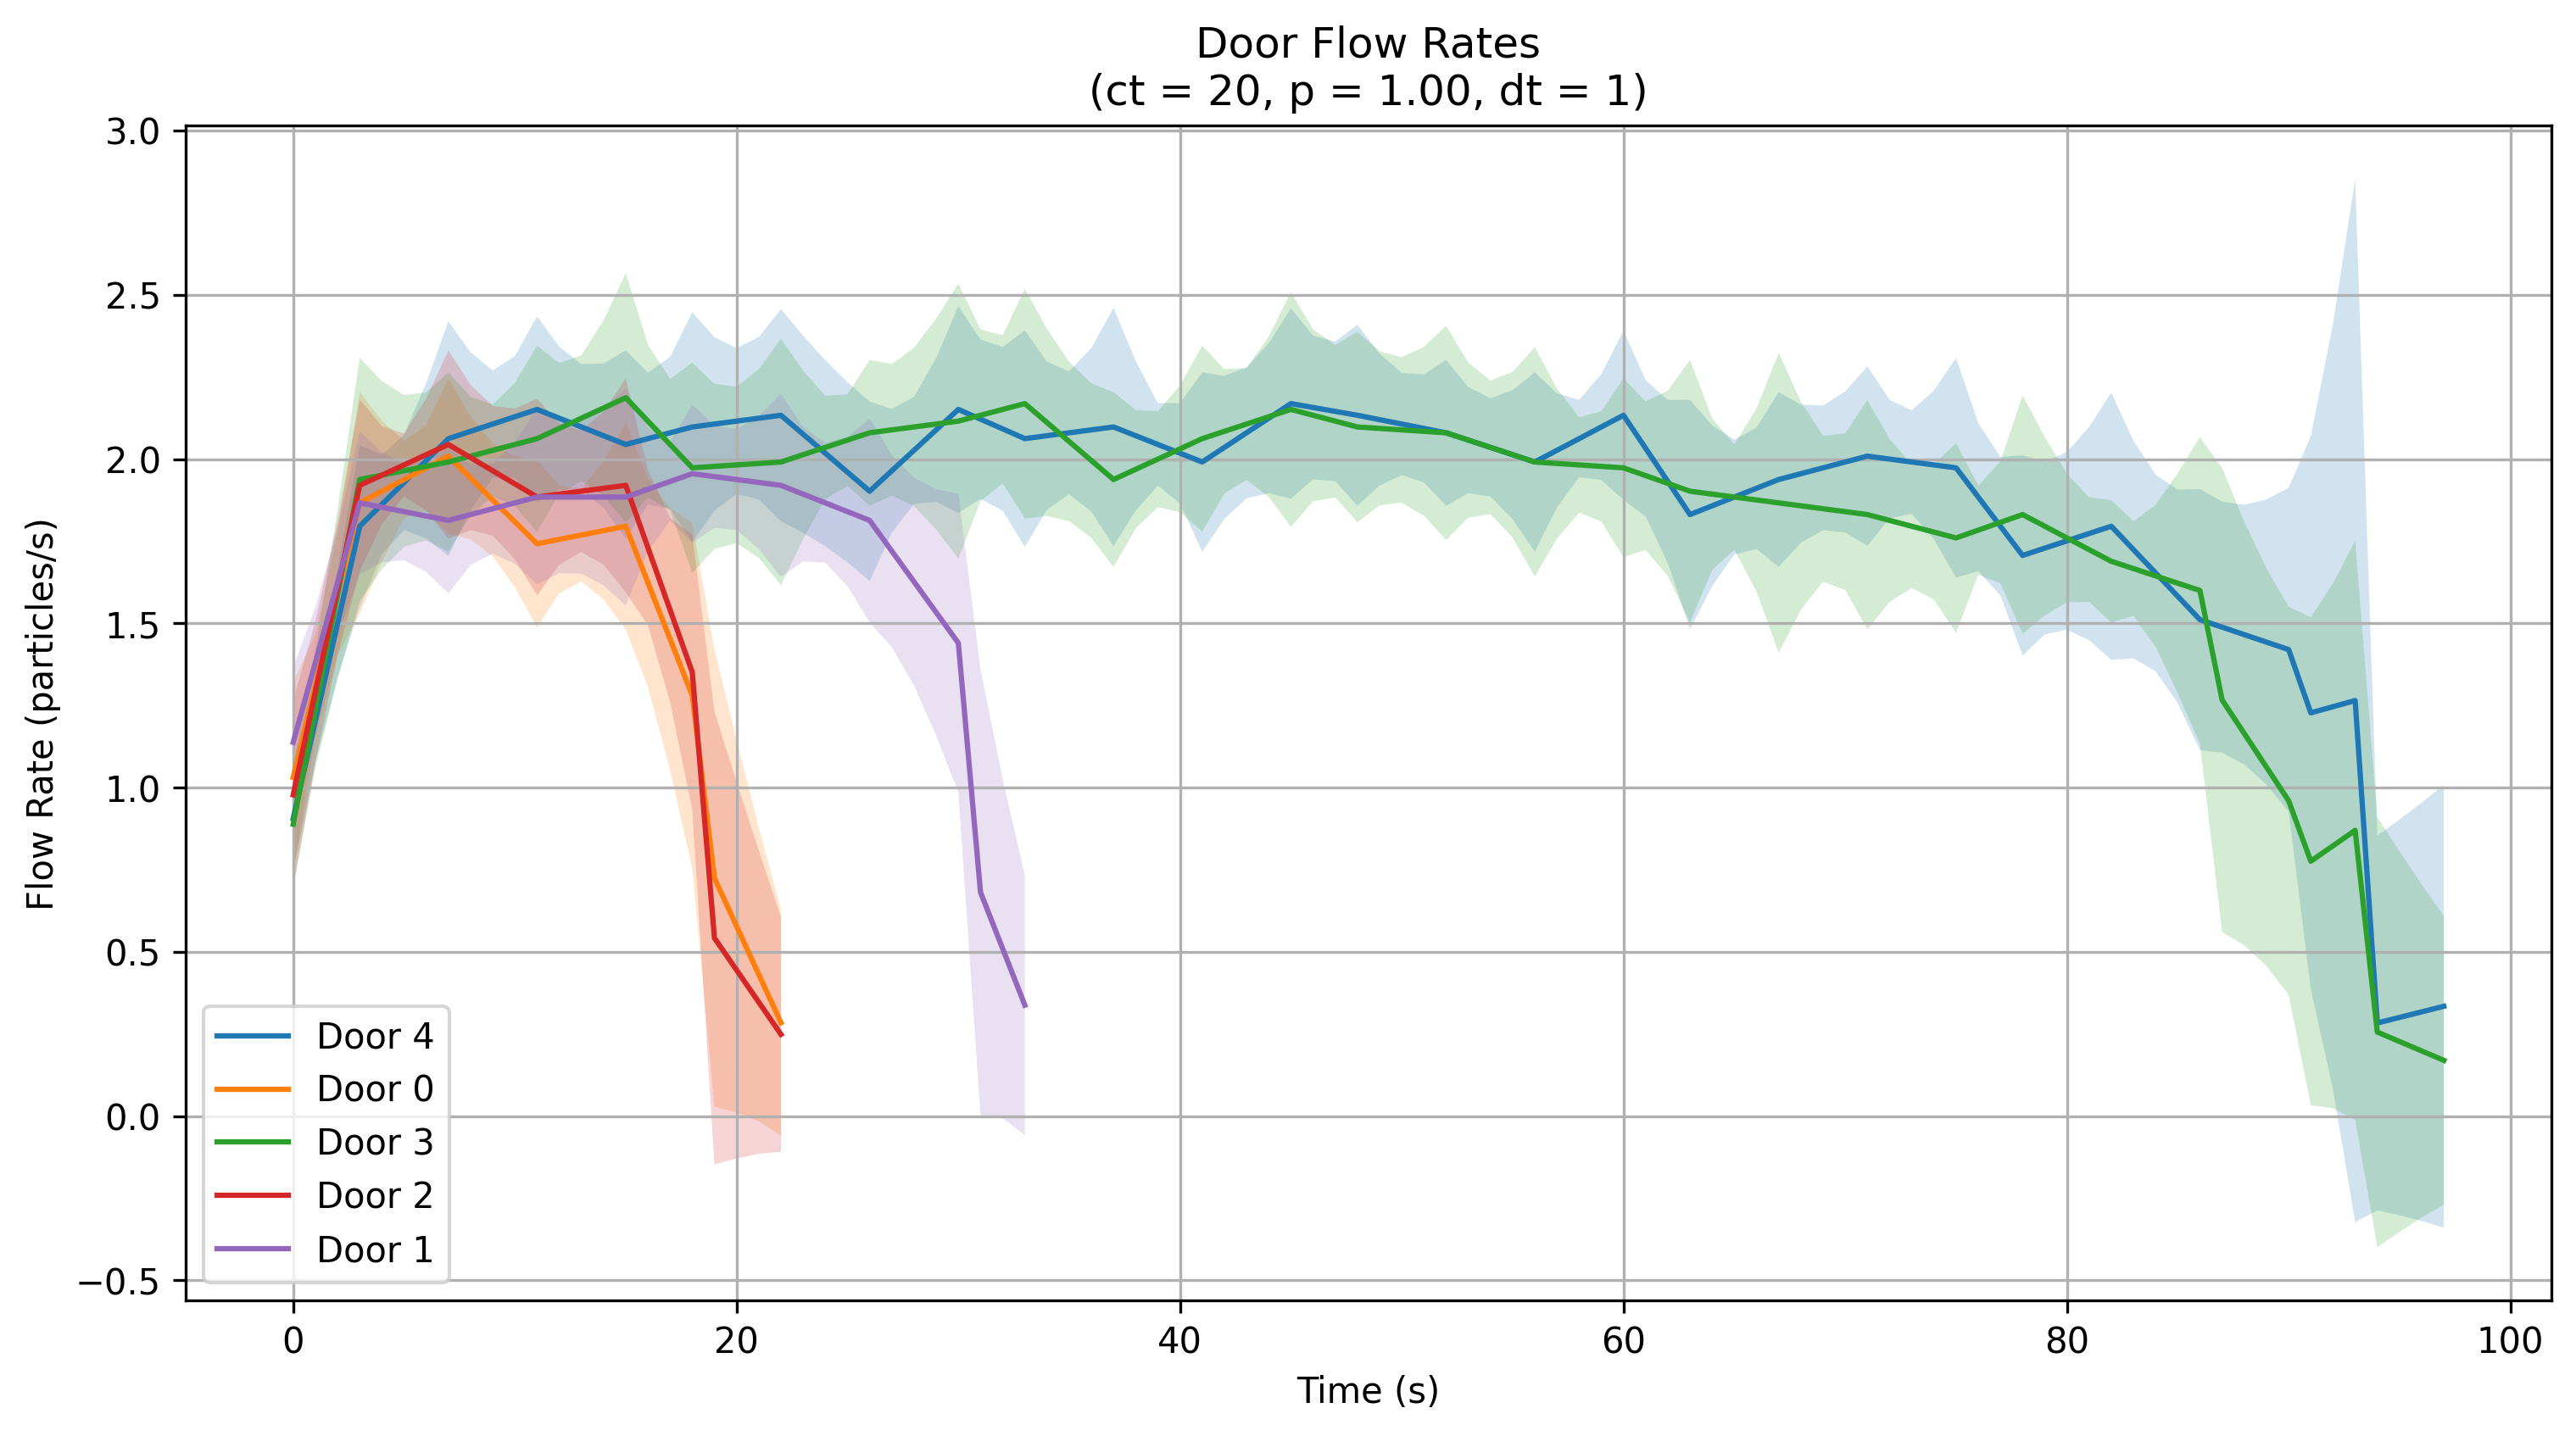
\includegraphics[width=0.6\textwidth]{img/door_flow_rates_t_20_&_p_1.00.png}
        \caption{Caudal promedio de partículas ($p=1.00$)}
    \end{figure}
\end{frame}

\begin{frame}{Caudal por Puerta ($p=0.50$)}
    \begin{figure}
        \centering
        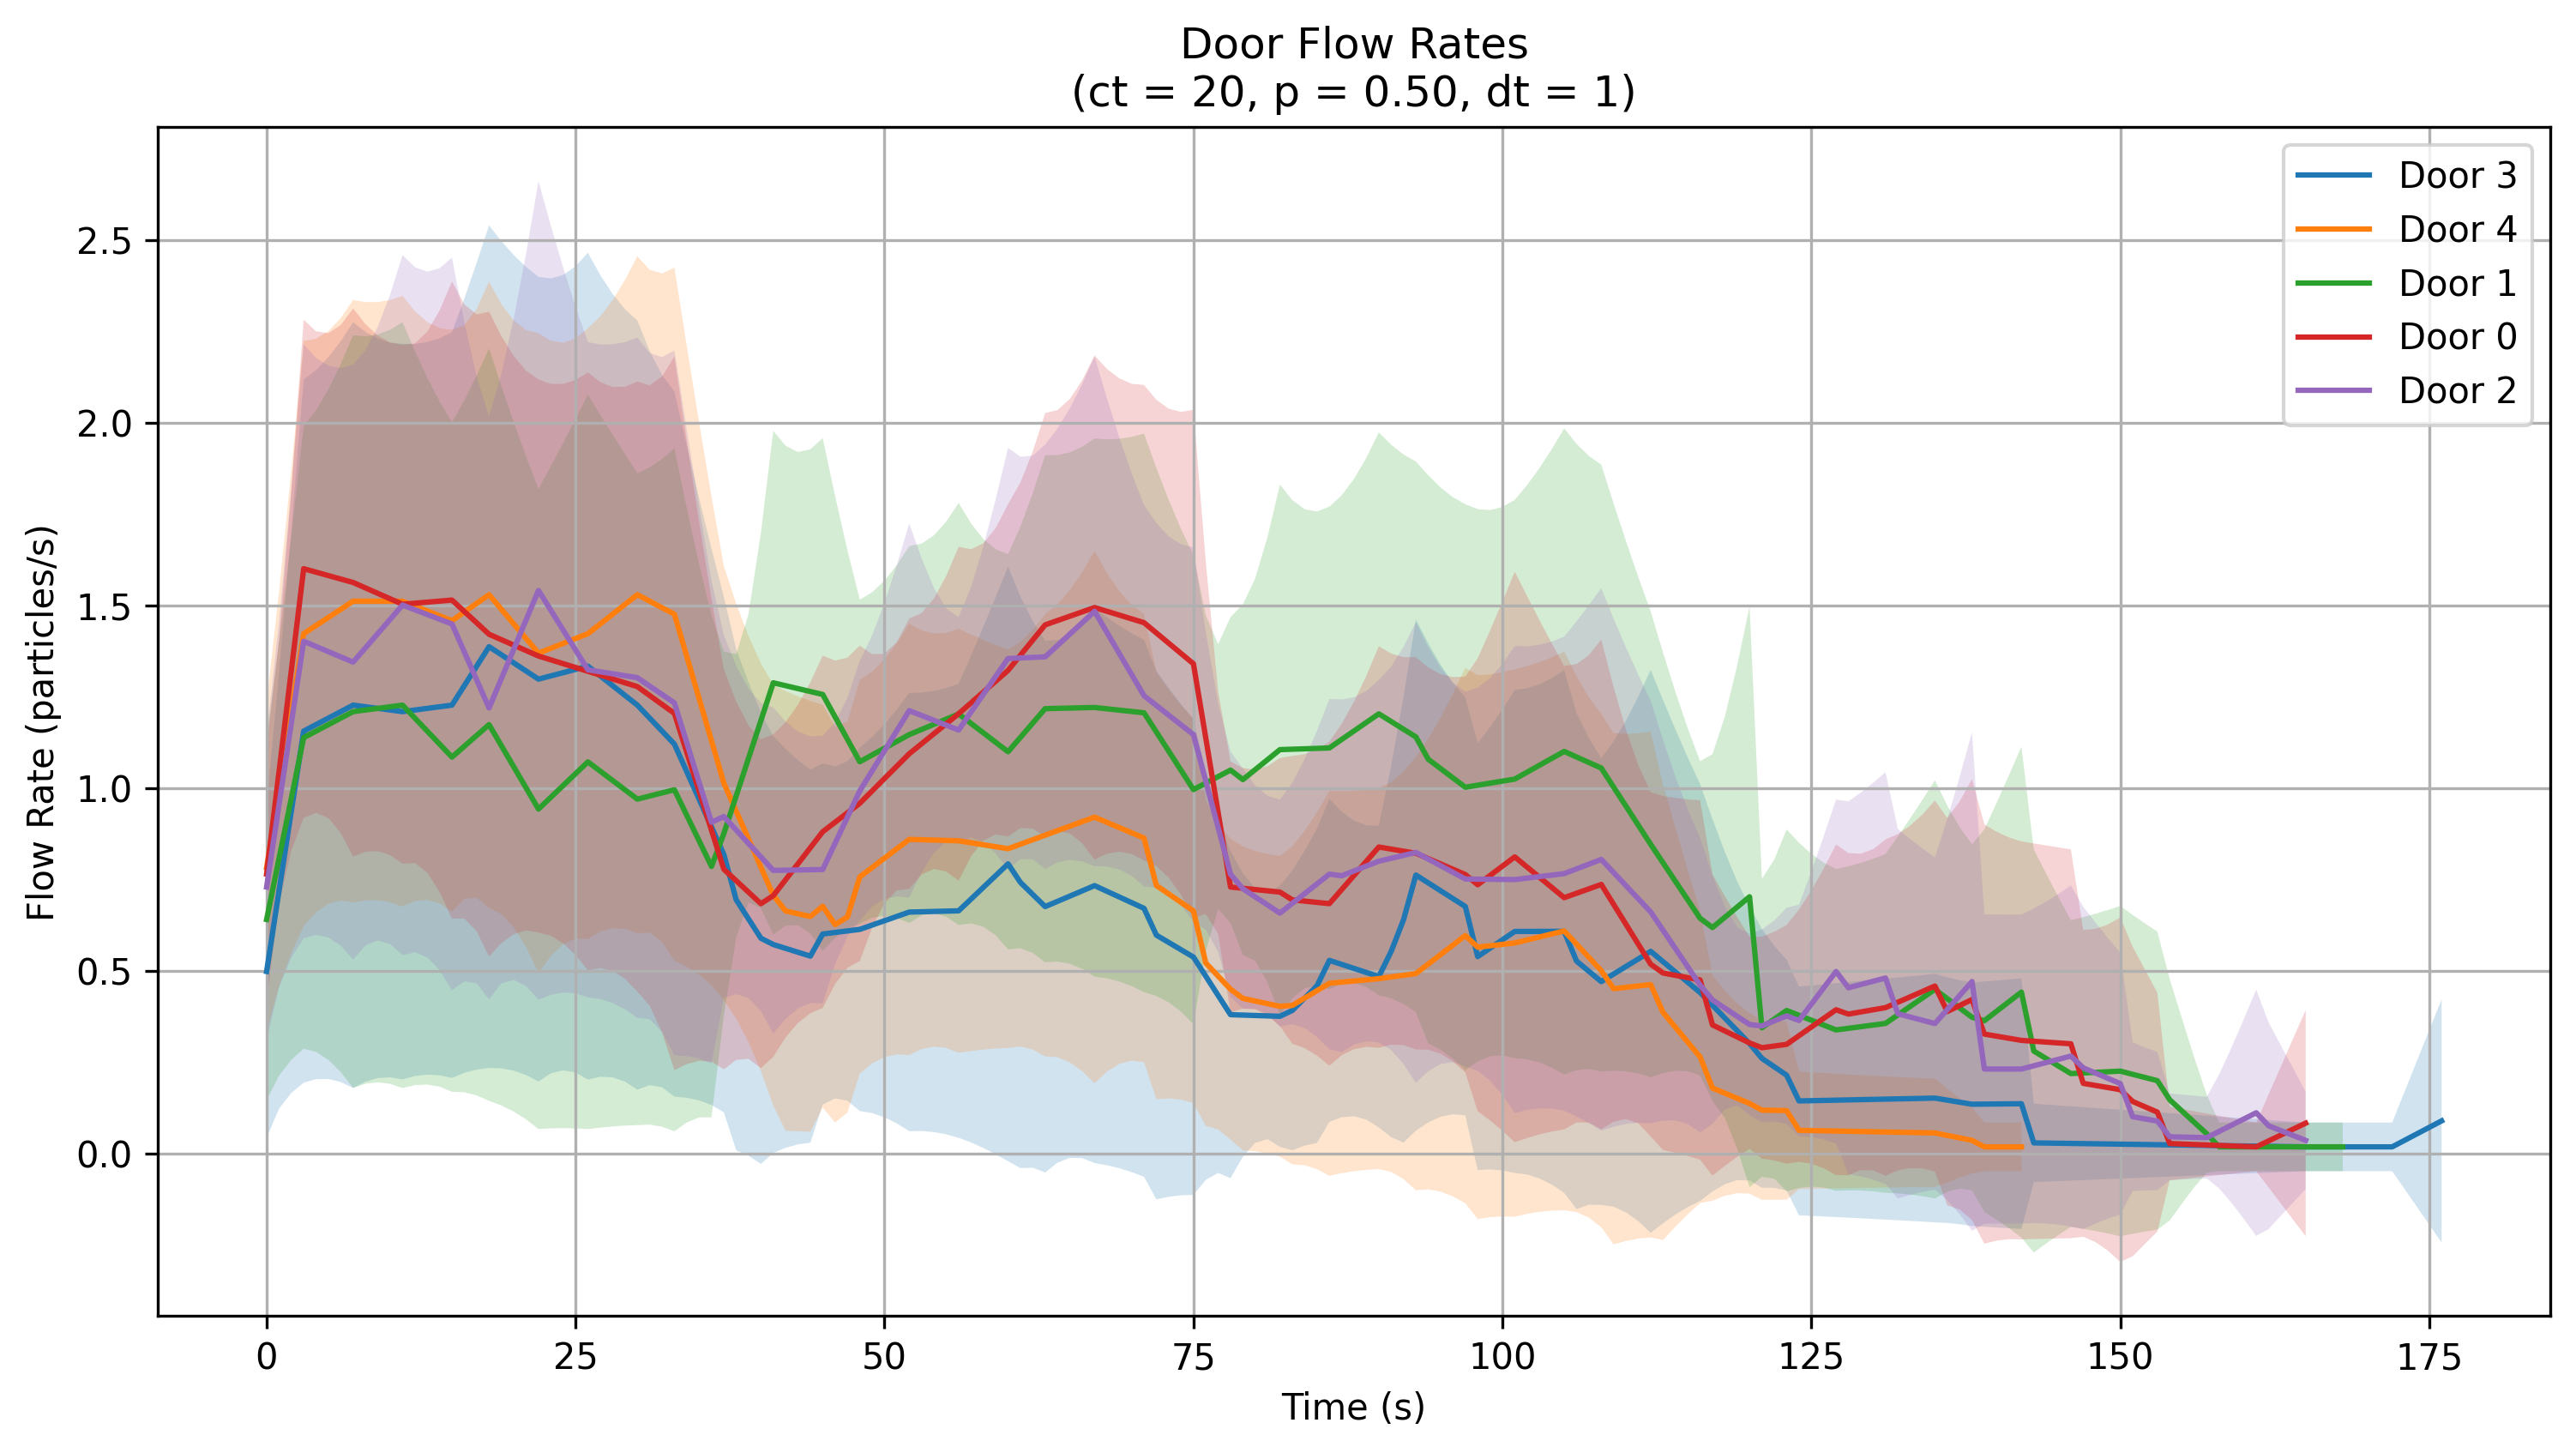
\includegraphics[width=0.6\textwidth]{img/door_flow_rates_t_20_&_p_0.50.png}
        \caption{Caudal promedio de partículas ($p=0.50$)}
    \end{figure}
\end{frame}

\begin{frame}{Caudal por Puerta ($p=0.00$)}
    \begin{figure}
        \centering
        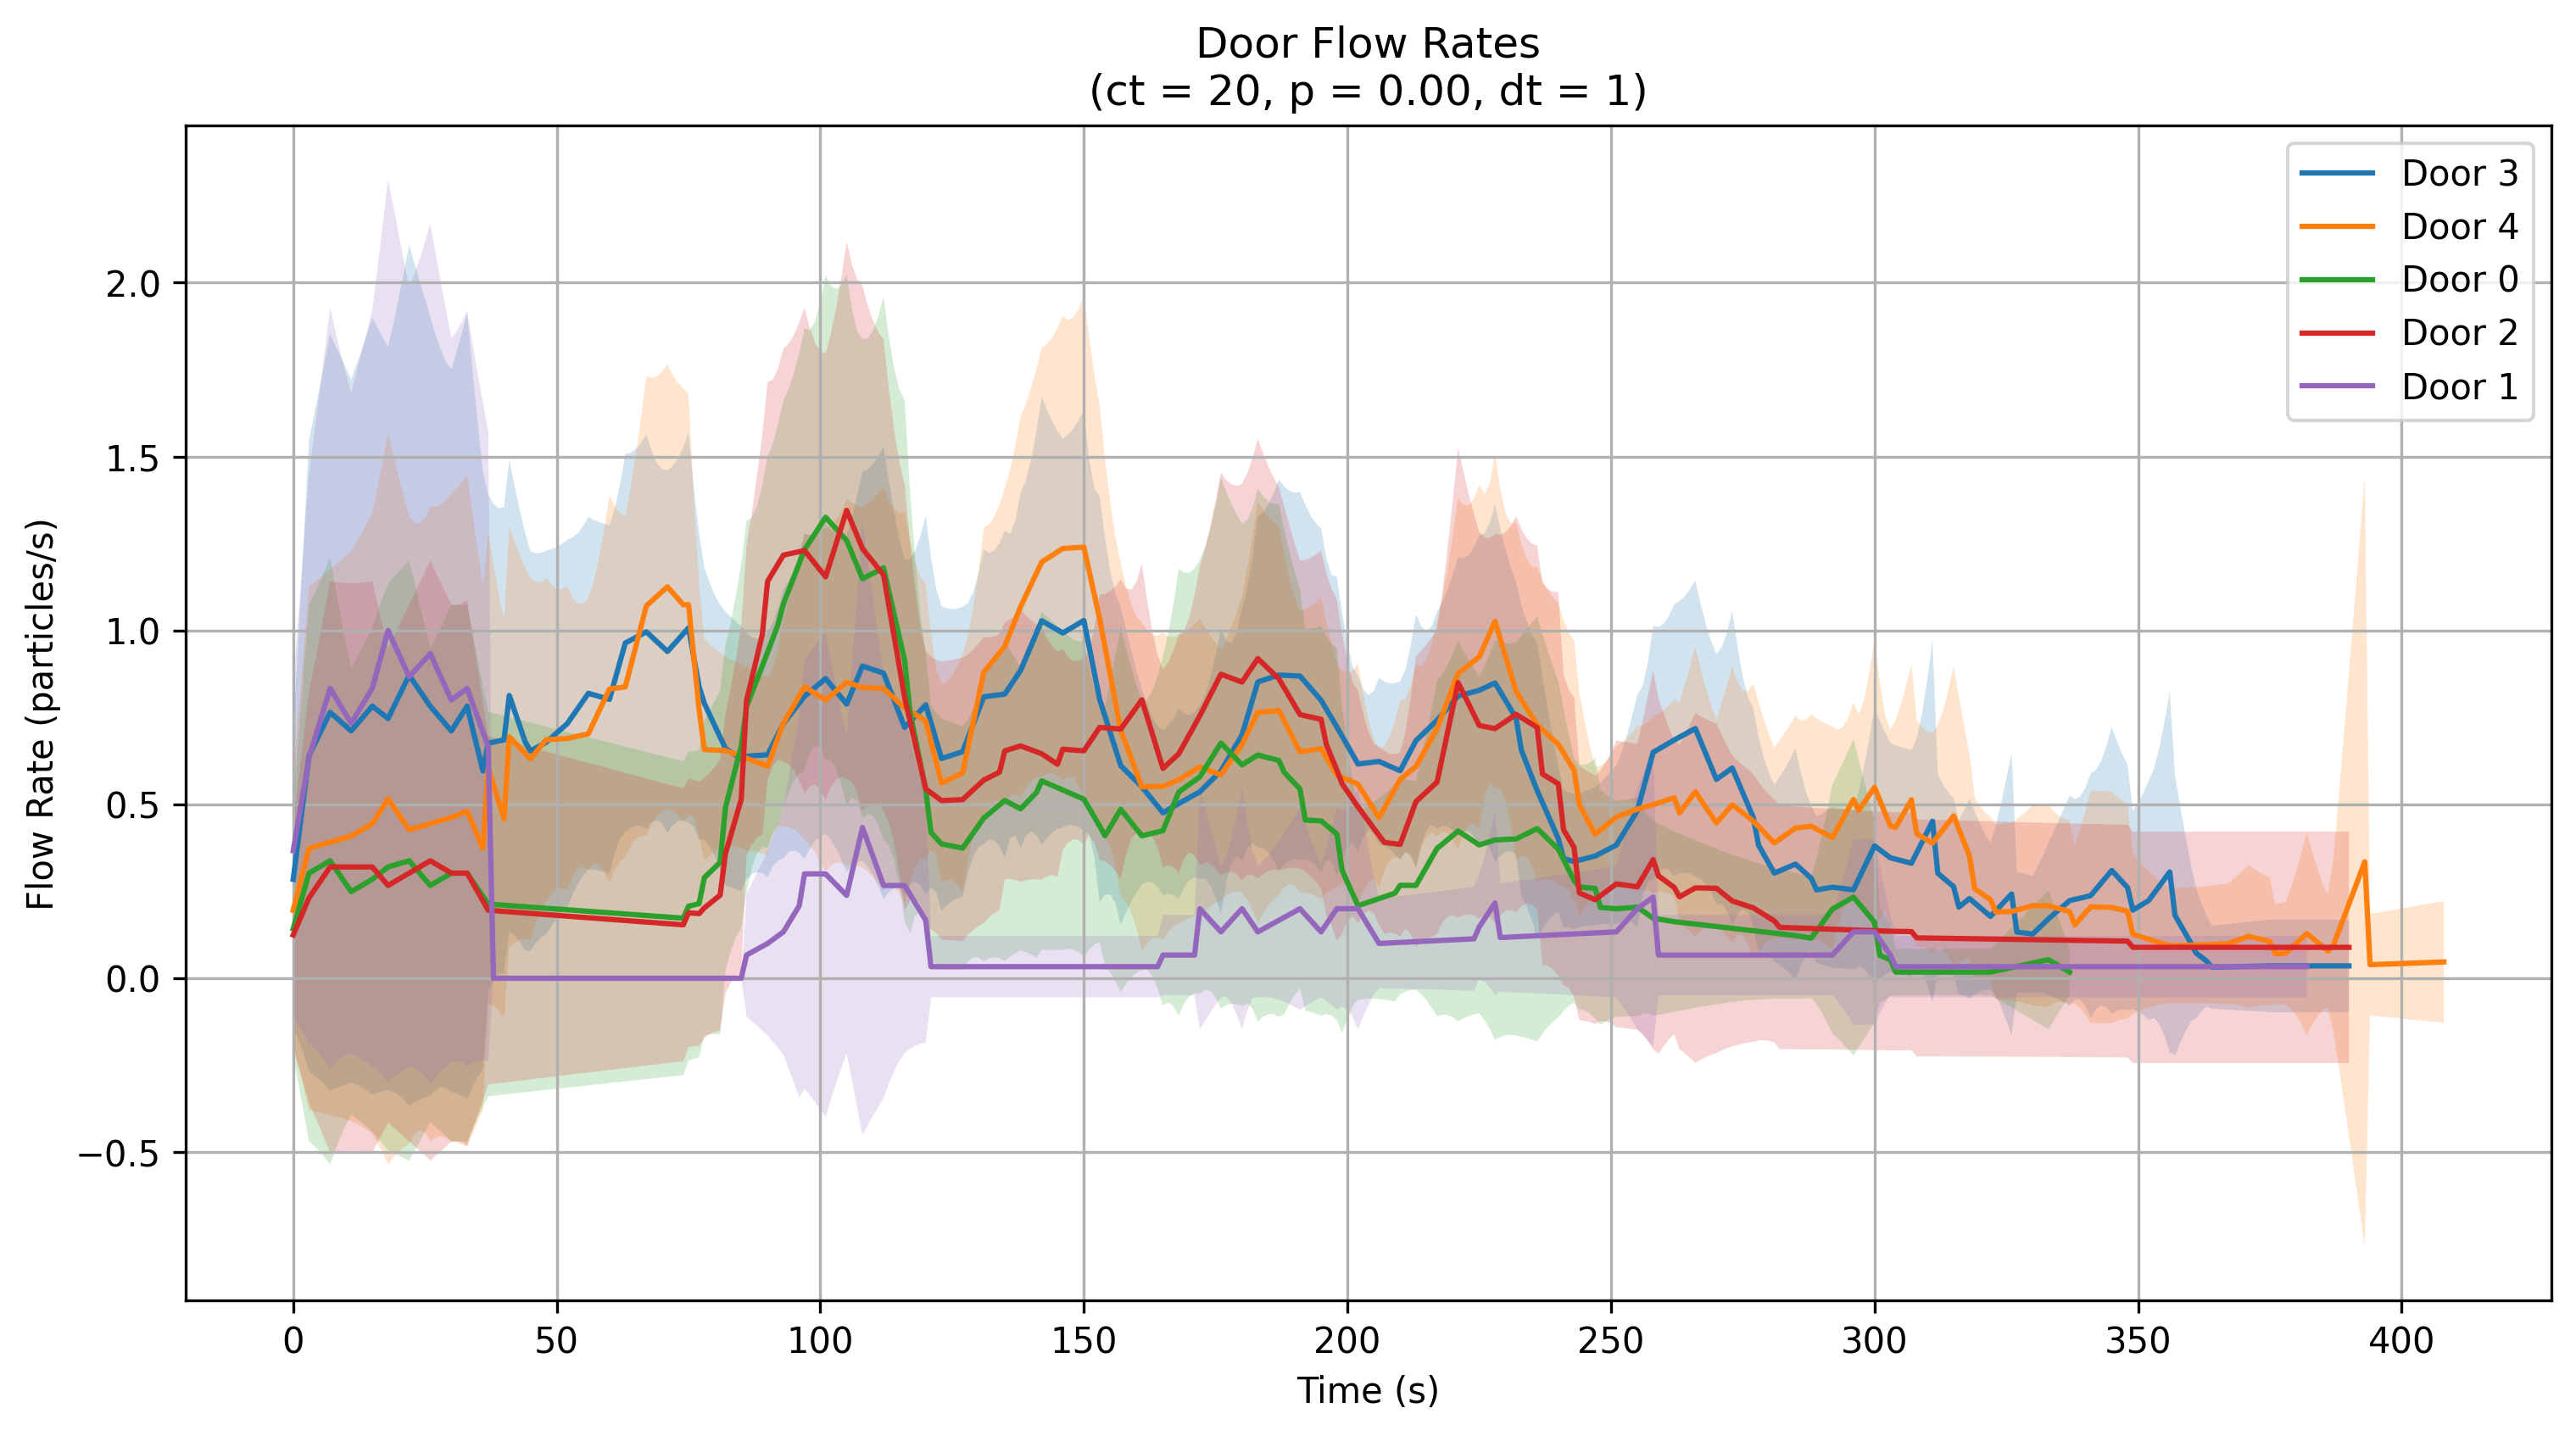
\includegraphics[width=0.6\textwidth]{img/door_flow_rates_t_20_&_p_0.00.png}
        \caption{Caudal promedio de partículas ($p=0.00$)}
    \end{figure}
\end{frame}


\begin{frame}{Densidad en función del tiempo}
    \begin{figure}
        \centering
        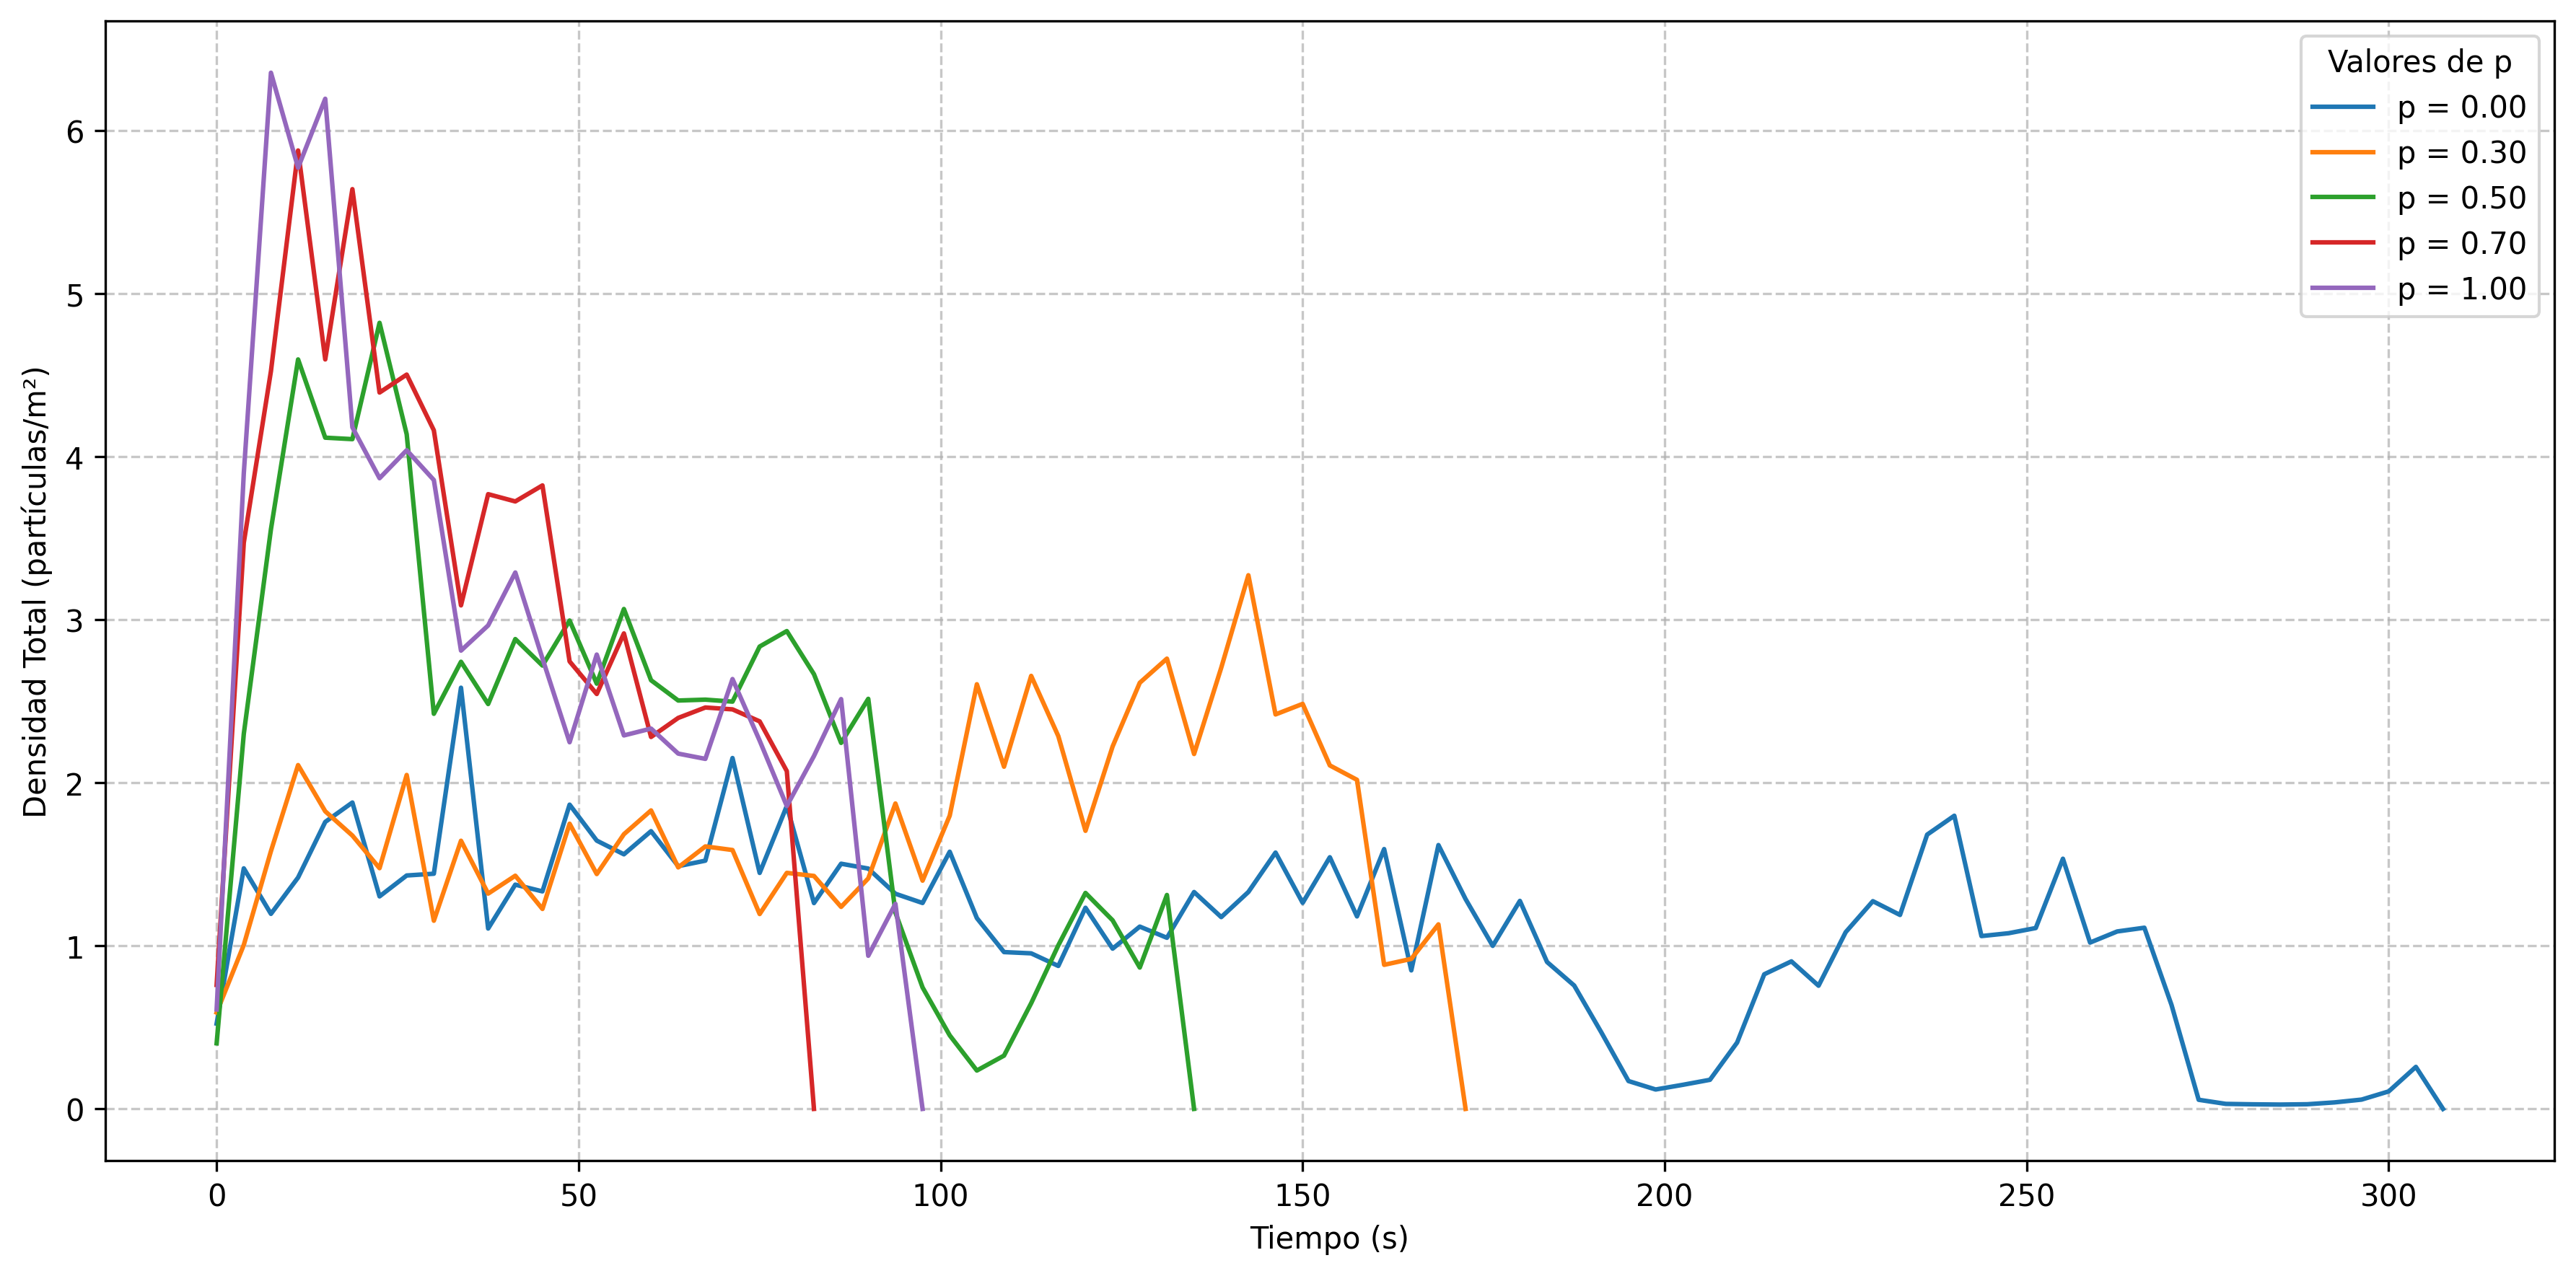
\includegraphics[width=0.6\textwidth]{img/density_vs_time_t45.png}
        \caption{Densidad en función del tiempo para $ct = 45$}
        \label{fig:flow_p100}
    \end{figure}
\end{frame}

\begin{frame}{Densidad en función de $p$}
    \begin{figure}
        \centering
        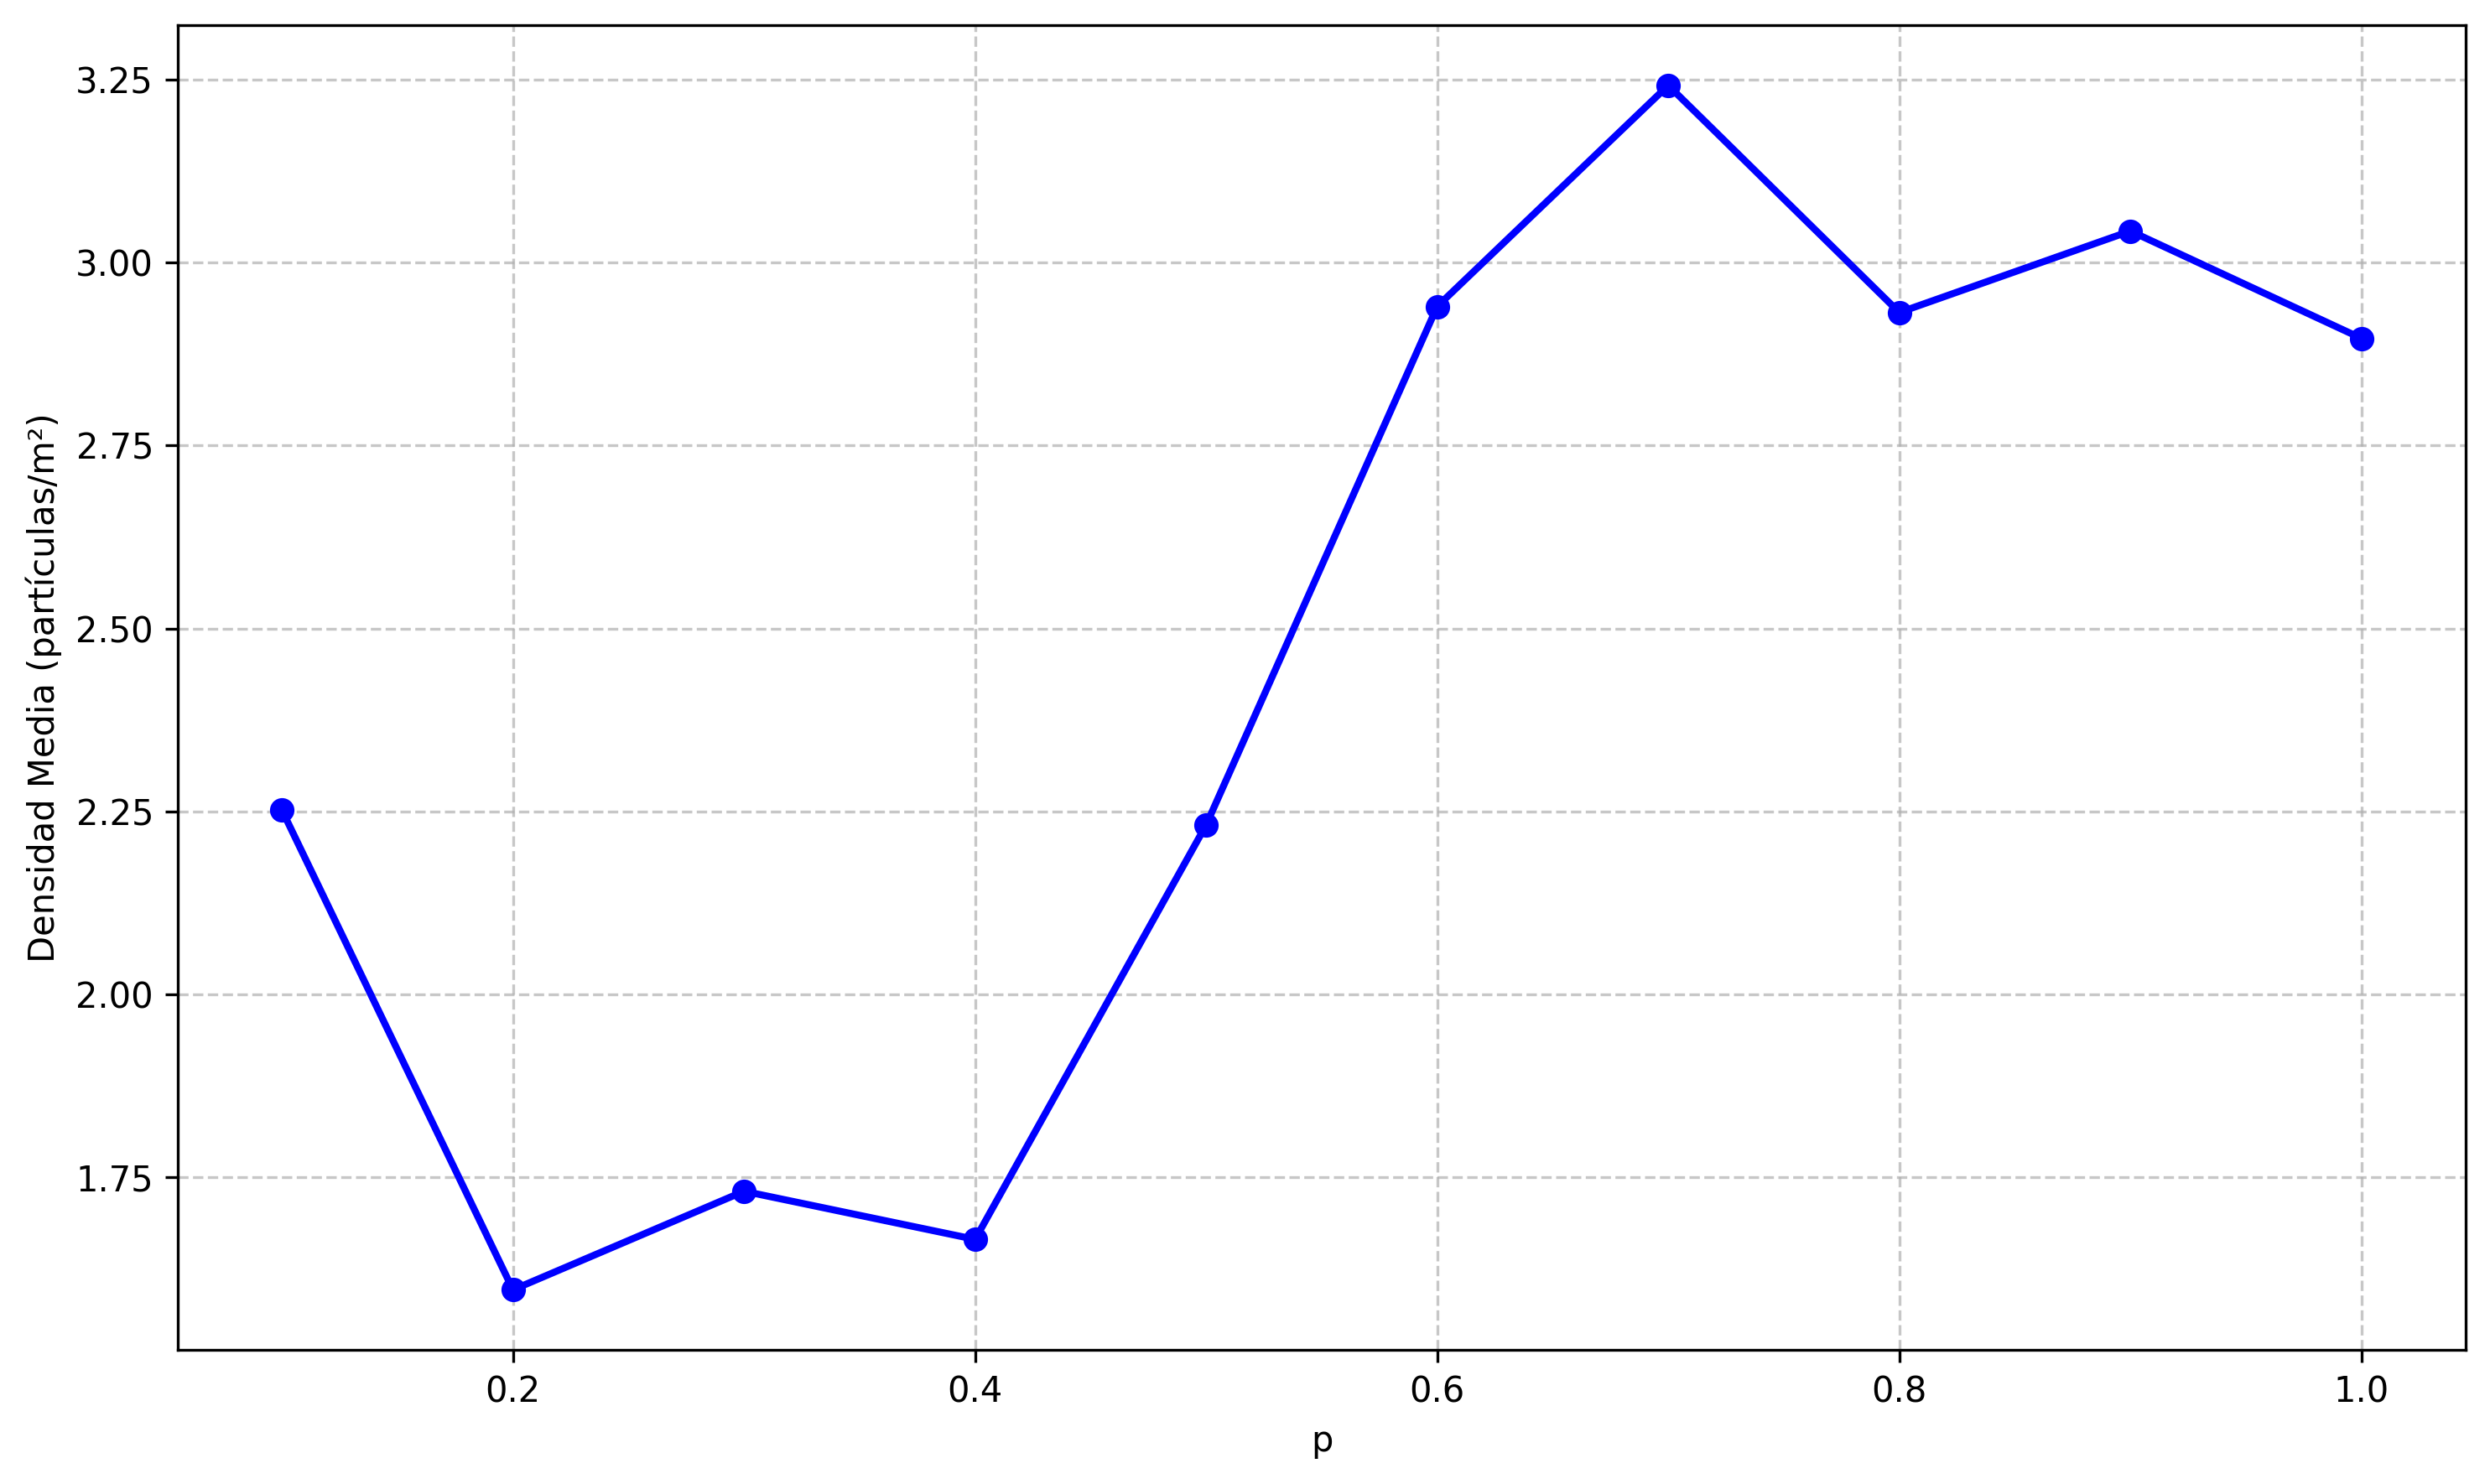
\includegraphics[width=0.6\textwidth]{img/average_density_t45.png}
        \caption{Densidad media en función de $p$ para $ct=45$}
    \end{figure}
\end{frame}

%\subsection{Análisis de Densidades por Puerta}

\begin{frame}{Análisis de Densidades por Puerta: $p = 1,0$ (Prioridad total a la Distancia)}
    \begin{figure}[H]
        \centering
        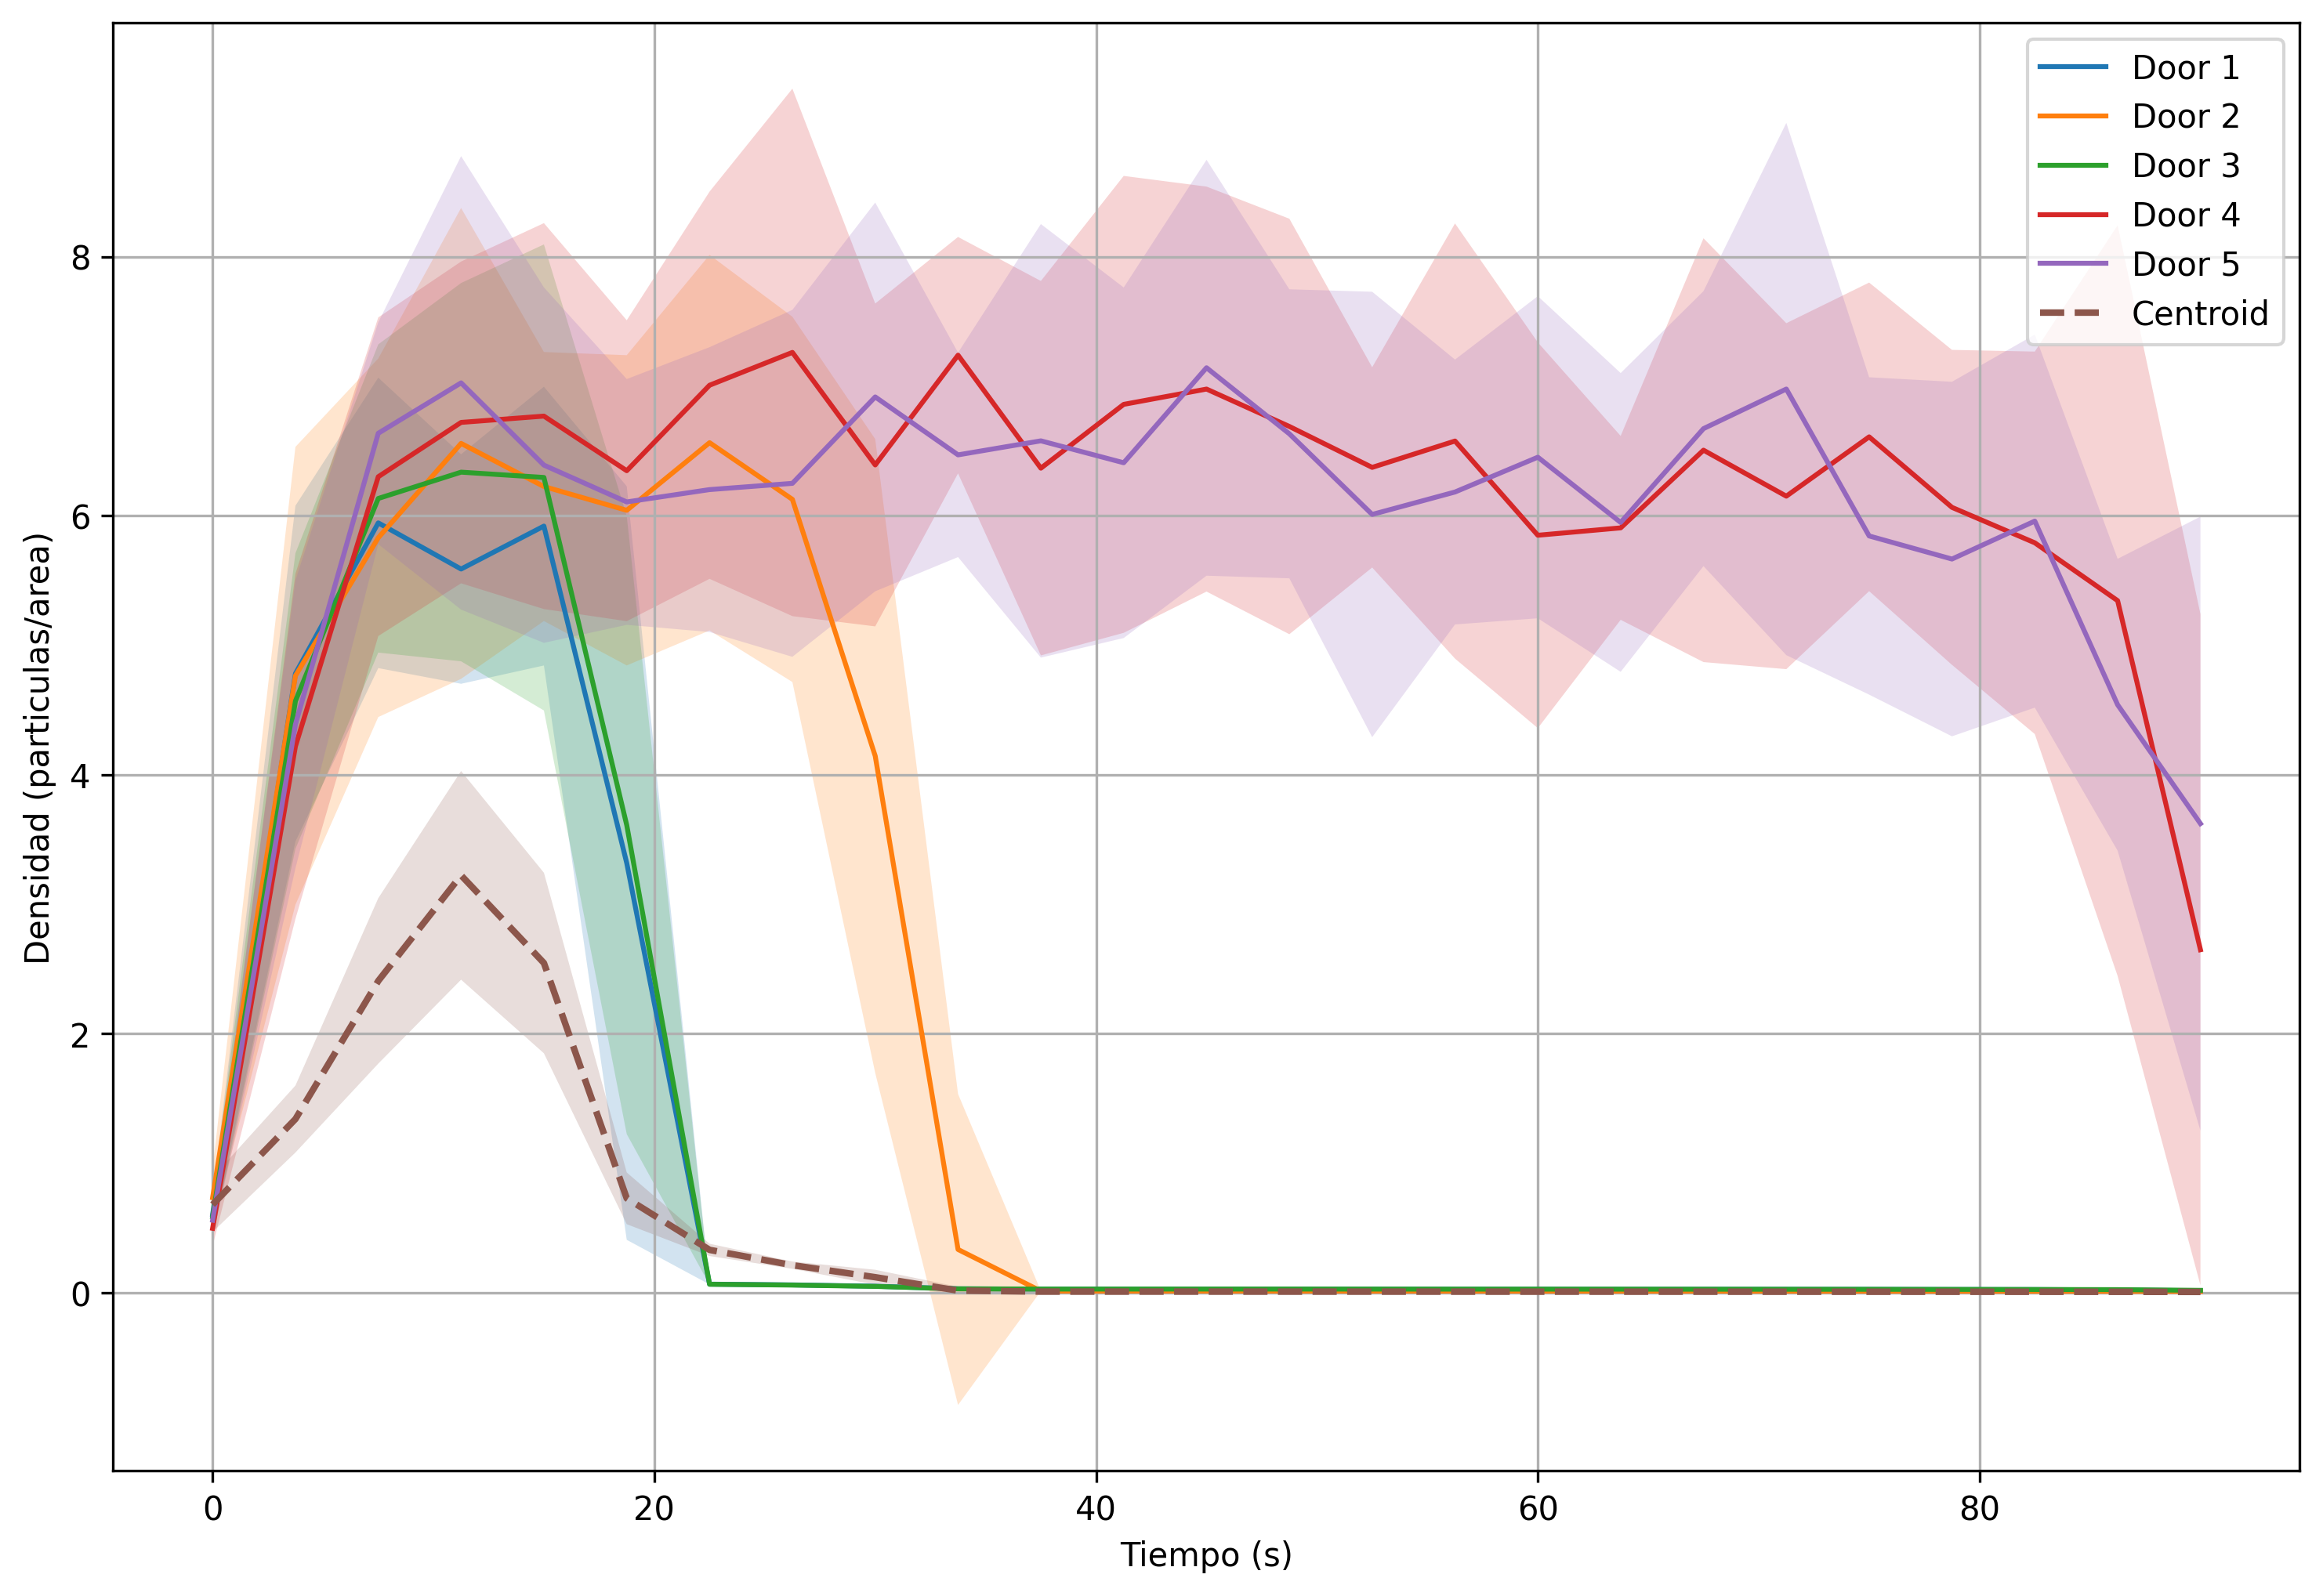
\includegraphics[width=0.6\textwidth]{img/circular_density_t_20_&_p_1.00.png}
        \caption{Densidad promedio de partículas en las proximidades de cada puerta para $p=1.00$}
        \label{fig:densidad_p100}
    \end{figure}
\end{frame}
\begin{frame}{Análisis de Densidades por Puerta: $p = 0.50$ (Balance entre Distancia y Densidad)}
    \begin{figure}[H]
        \centering
        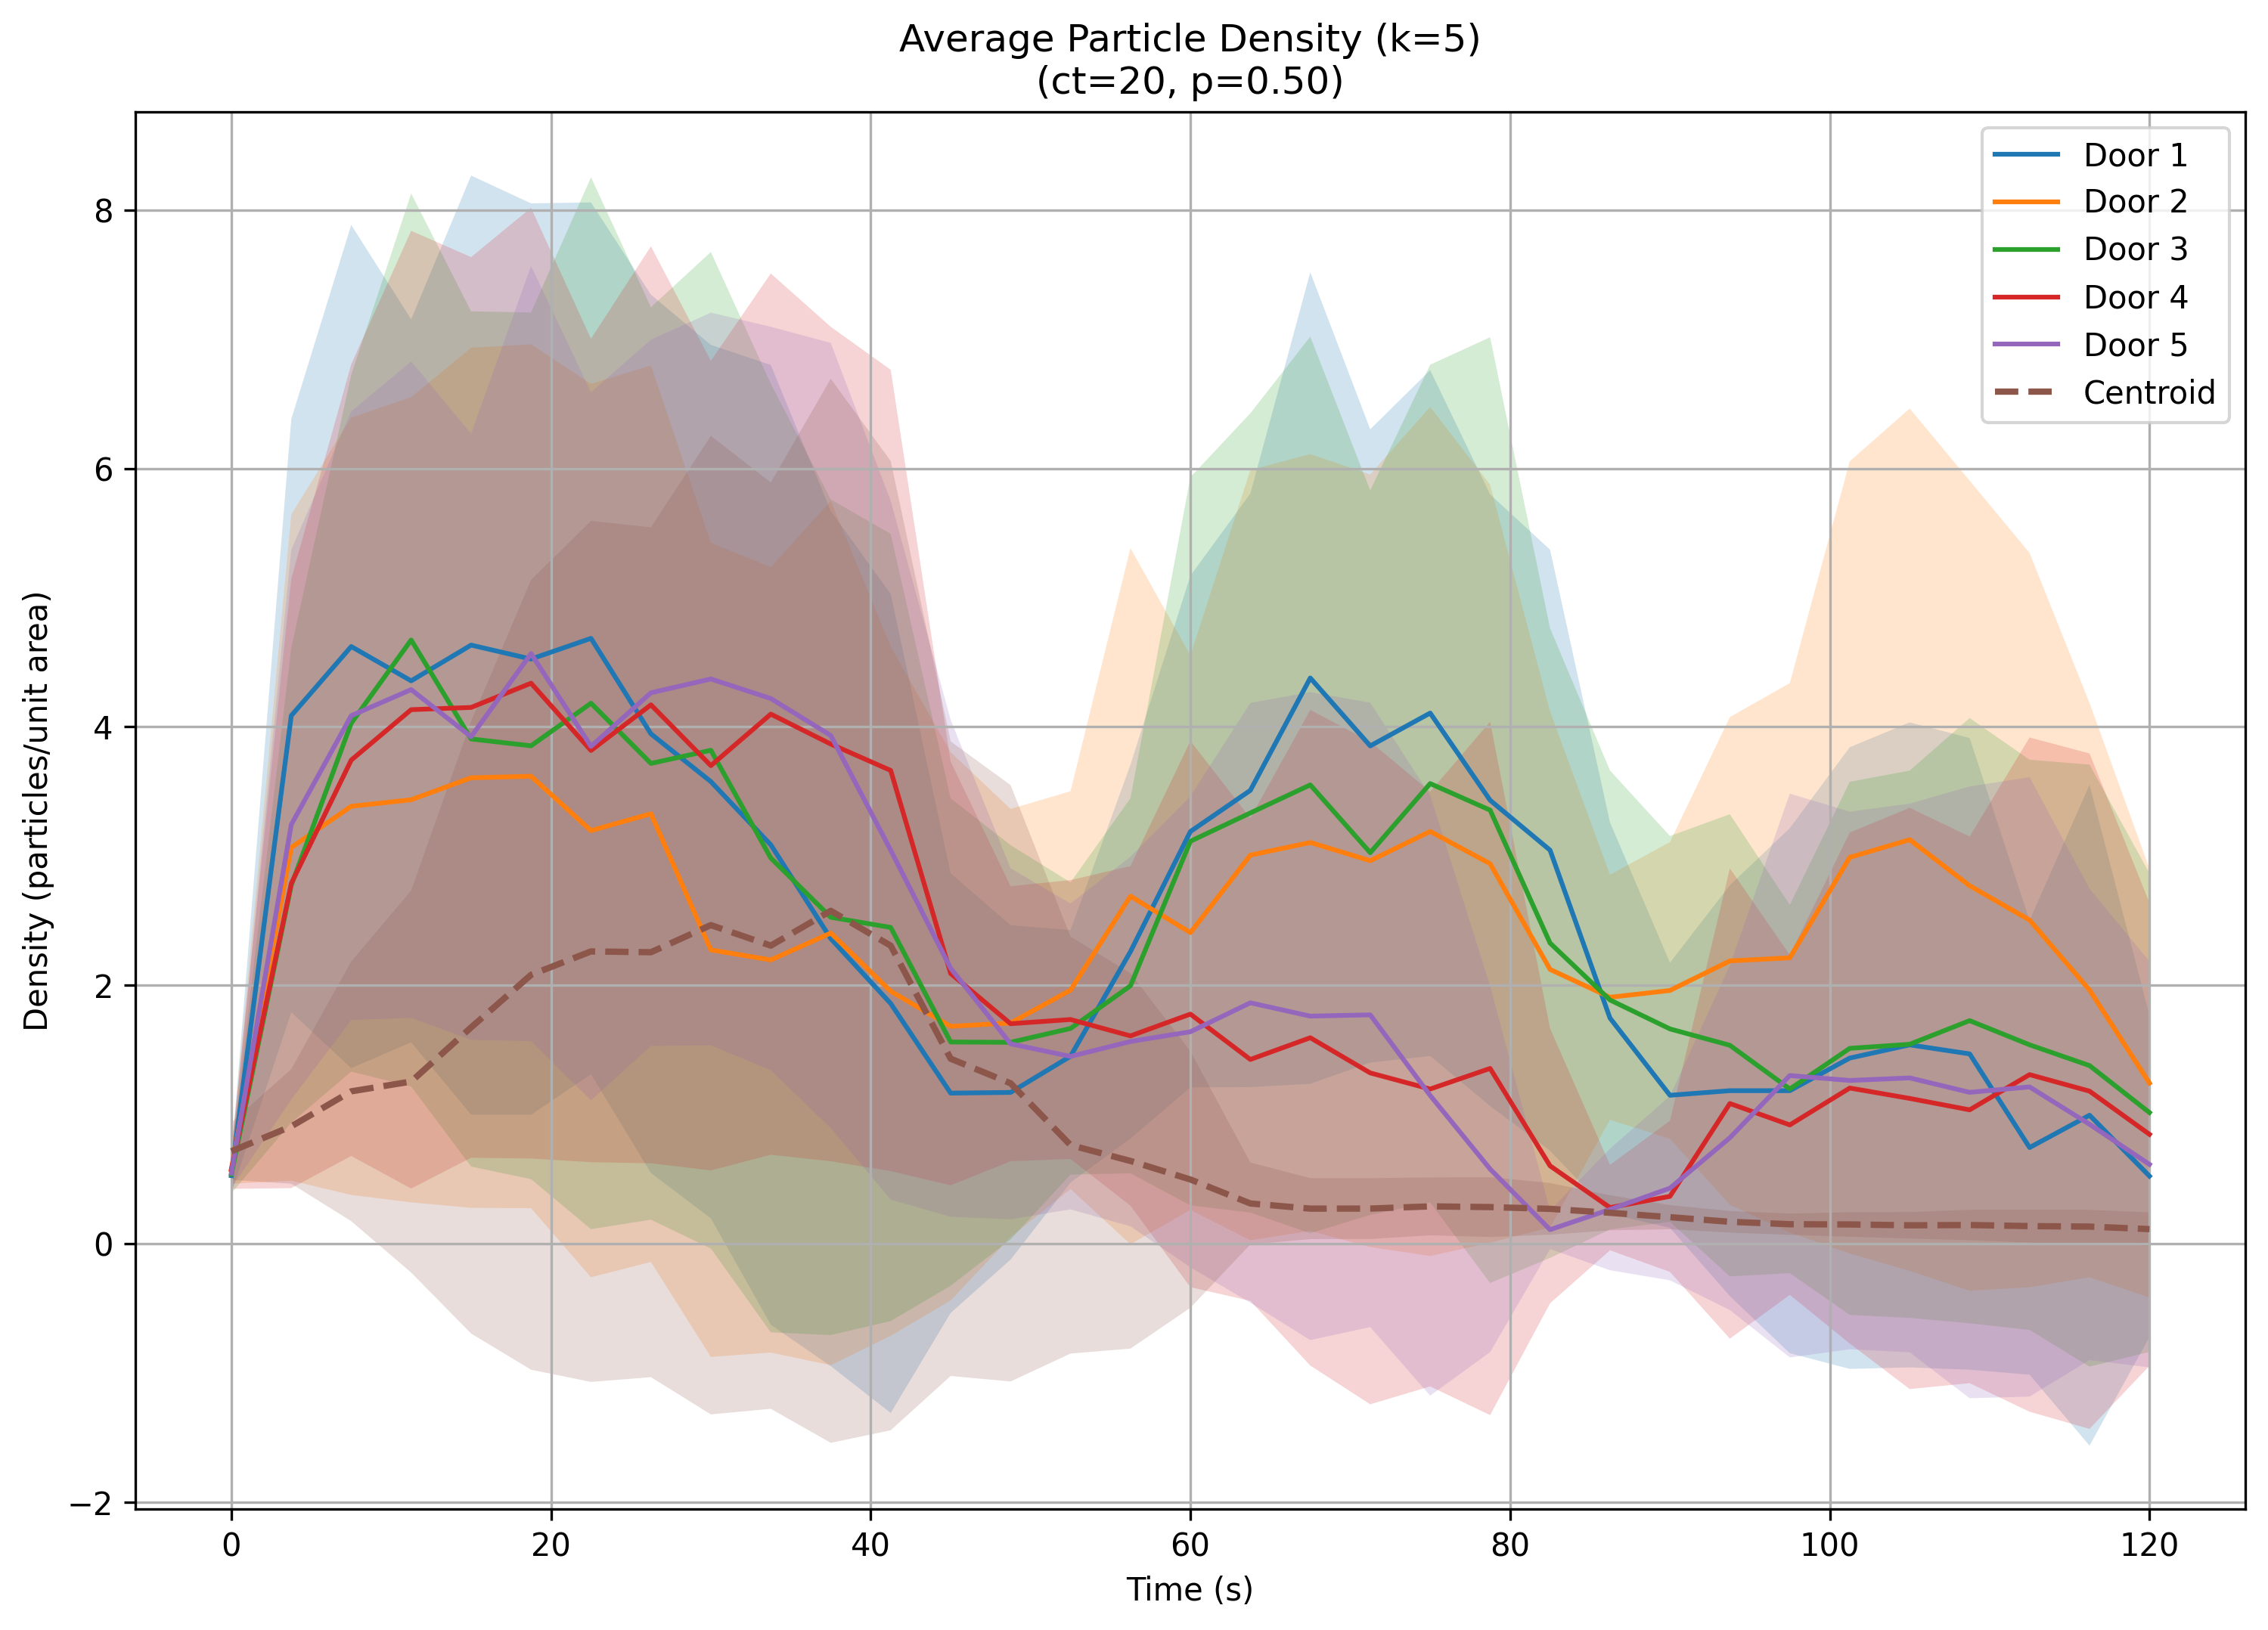
\includegraphics[width=0.6\textwidth]{img/circular_density_t_20_&_p_0.50.png}
        \caption{Densidad promedio de partículas en las proximidades de cada puerta para $p=0.50$}
        \label{fig:densidad_p050}
    \end{figure}
\end{frame}
\begin{frame}{Análisis de Densidades por Puerta: $p = 0.00$ (Prioridad total a la Densidad)}
    \begin{figure}[H]
        \centering
        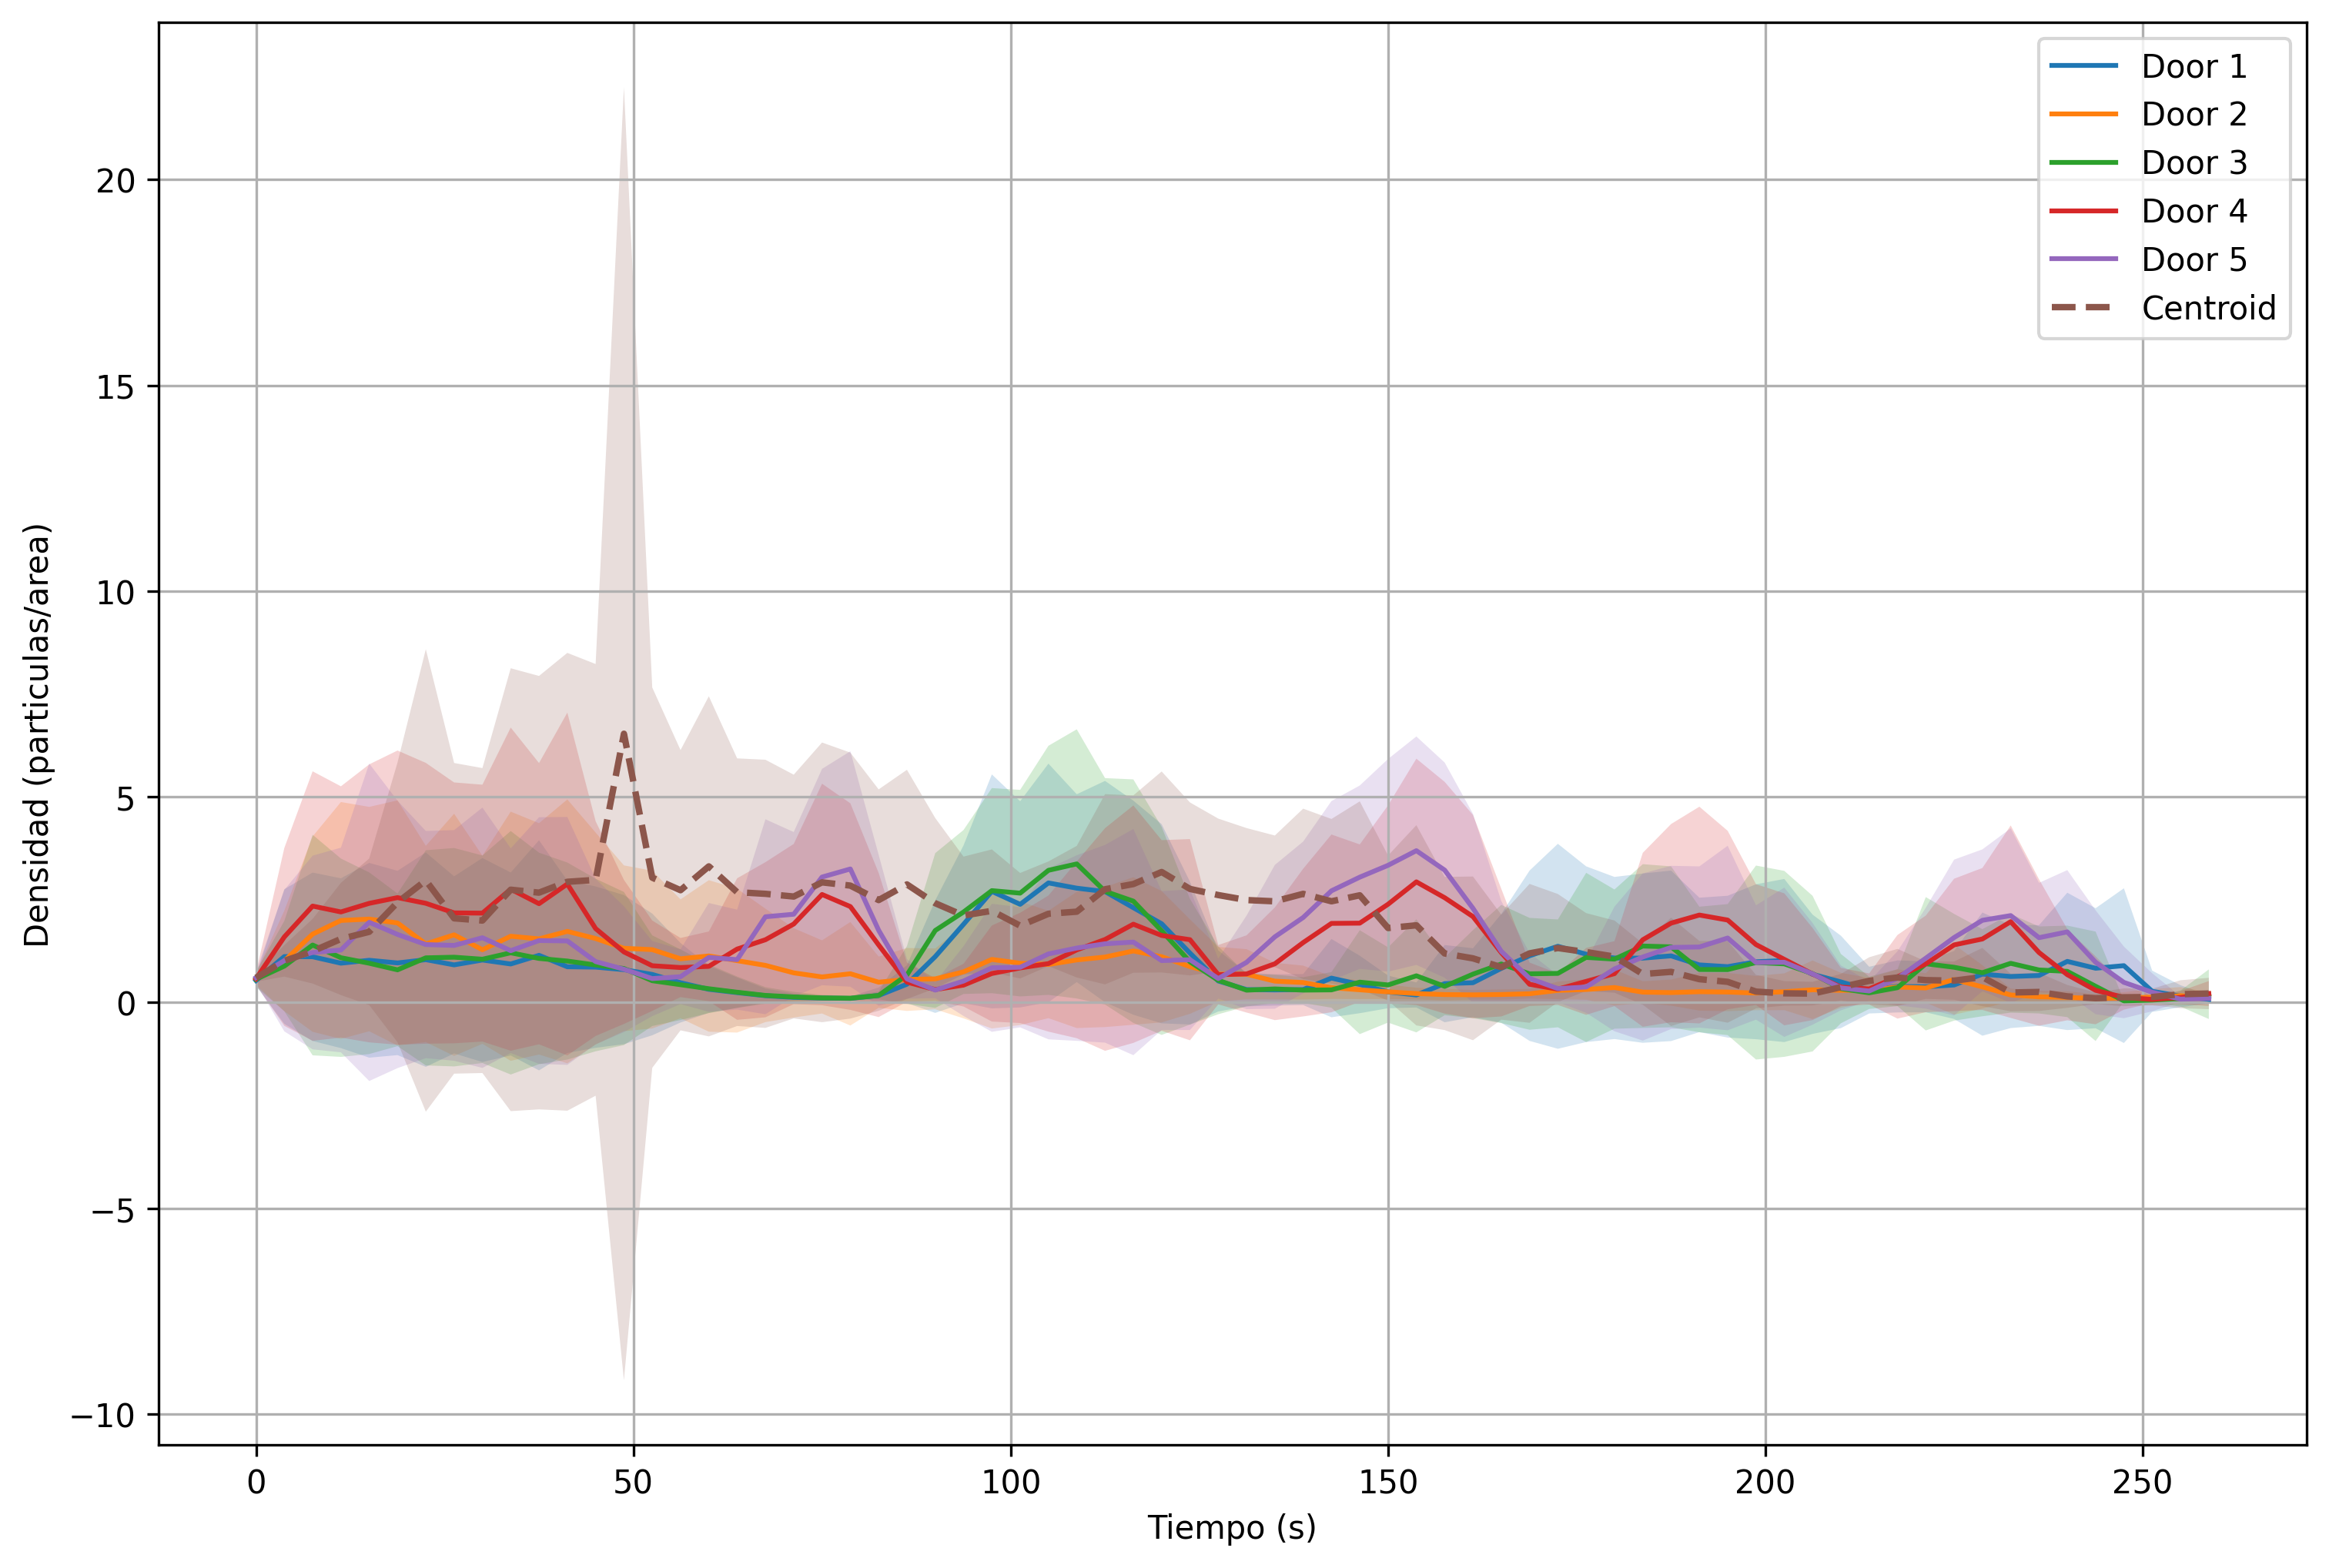
\includegraphics[width=0.6\textwidth]{img/circular_density_t_20_&_p_0.00.png}
        \caption{Densidad promedio de partículas en las proximidades de cada puerta para $p=0.00$}
        \label{fig:densidad_p000}
    \end{figure}
\end{frame}


\begin{frame}{Coeficiente de uniformidad en función de $p$}
    \begin{figure}[H]
        \centering
        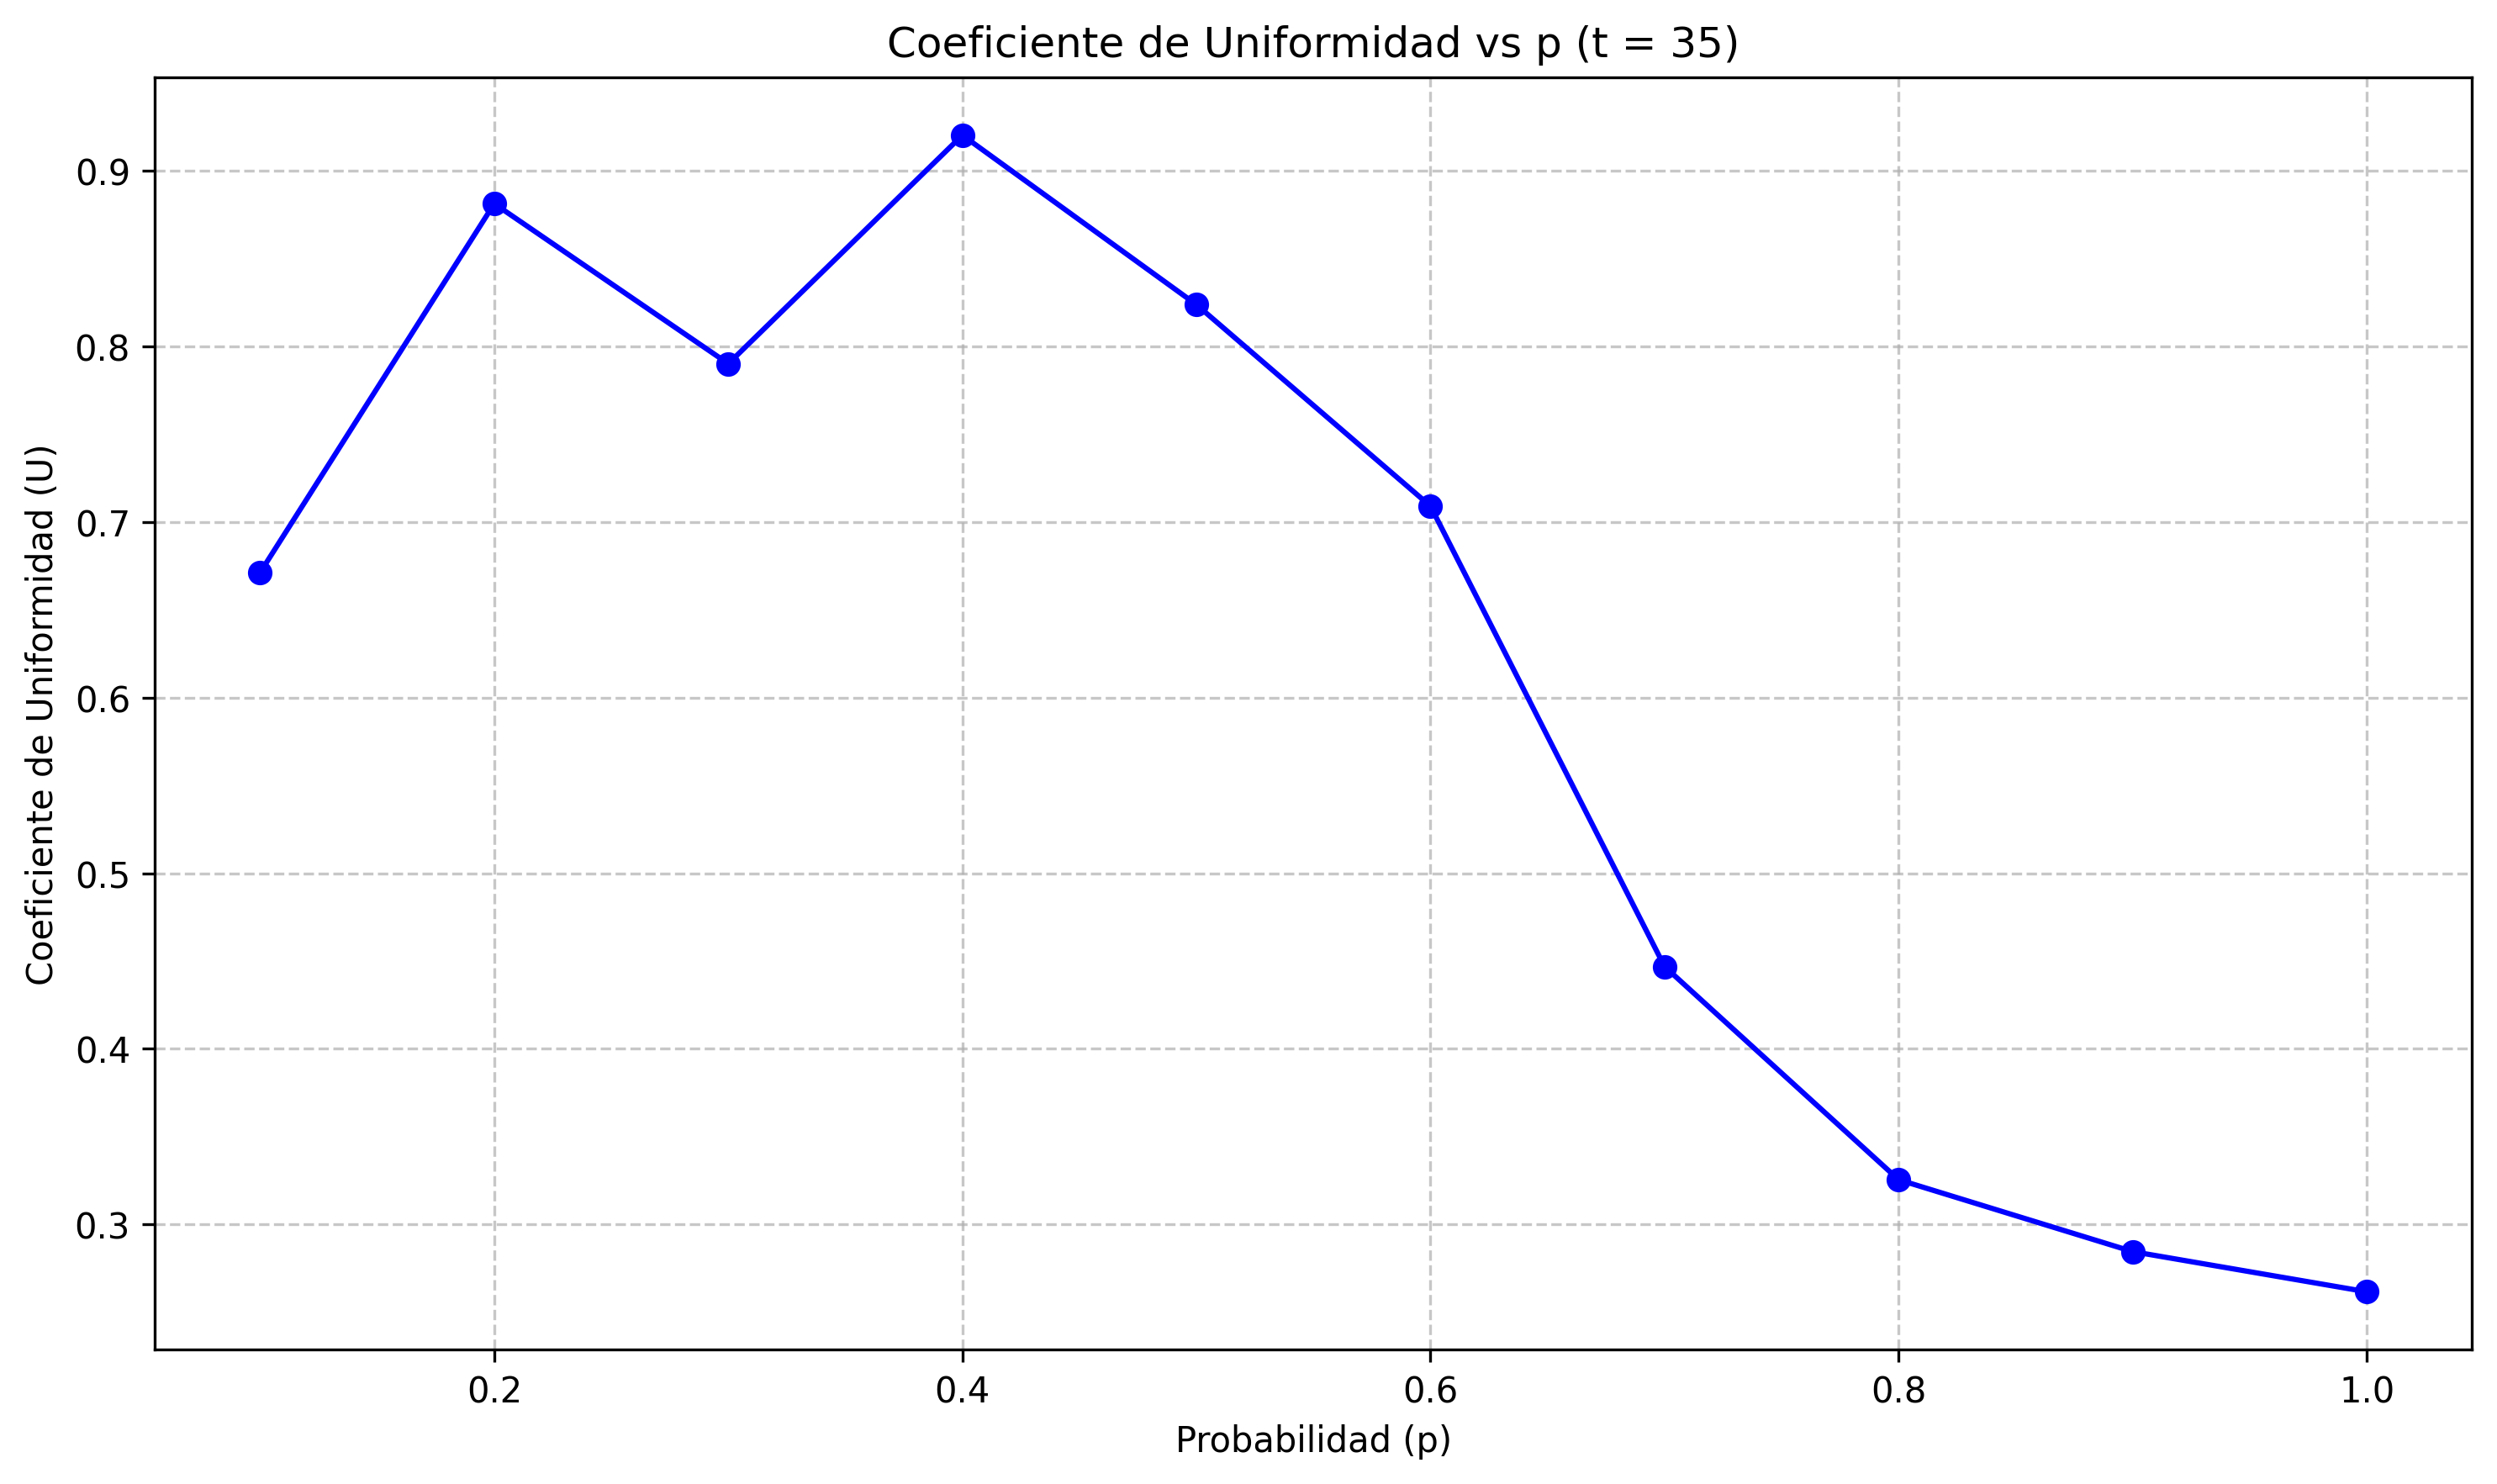
\includegraphics[width=0.6\textwidth]{img/uniformity_vs_p_t35.png}
        \caption{Coeficiente de uniformidad para $ct=35$}
        \label{fig:flow_p100}
    \end{figure}
\end{frame}

\begin{frame}{Análisis del Tiempo de Evacuación en función del Tiempo de Re-decisión}
    \begin{figure}[H]
        \centering
        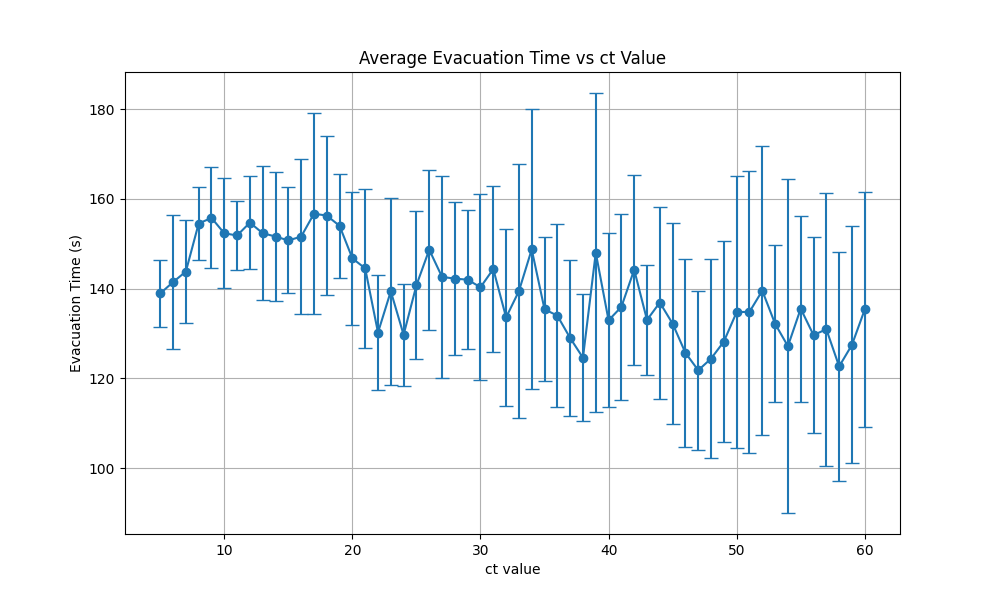
\includegraphics[width=0.6\textwidth]{img/evacuation_times_p_0.5.png}
        \caption{Tiempo promedio de evacuación en función del tiempo de re-decisión ($ct$) para $p=0.50$}
        \label{fig:evac_time_ct}
    \end{figure}    
\end{frame}

\begin{frame}{Caudal en función de $ct$}
    \begin{figure}[H]
        \centering
        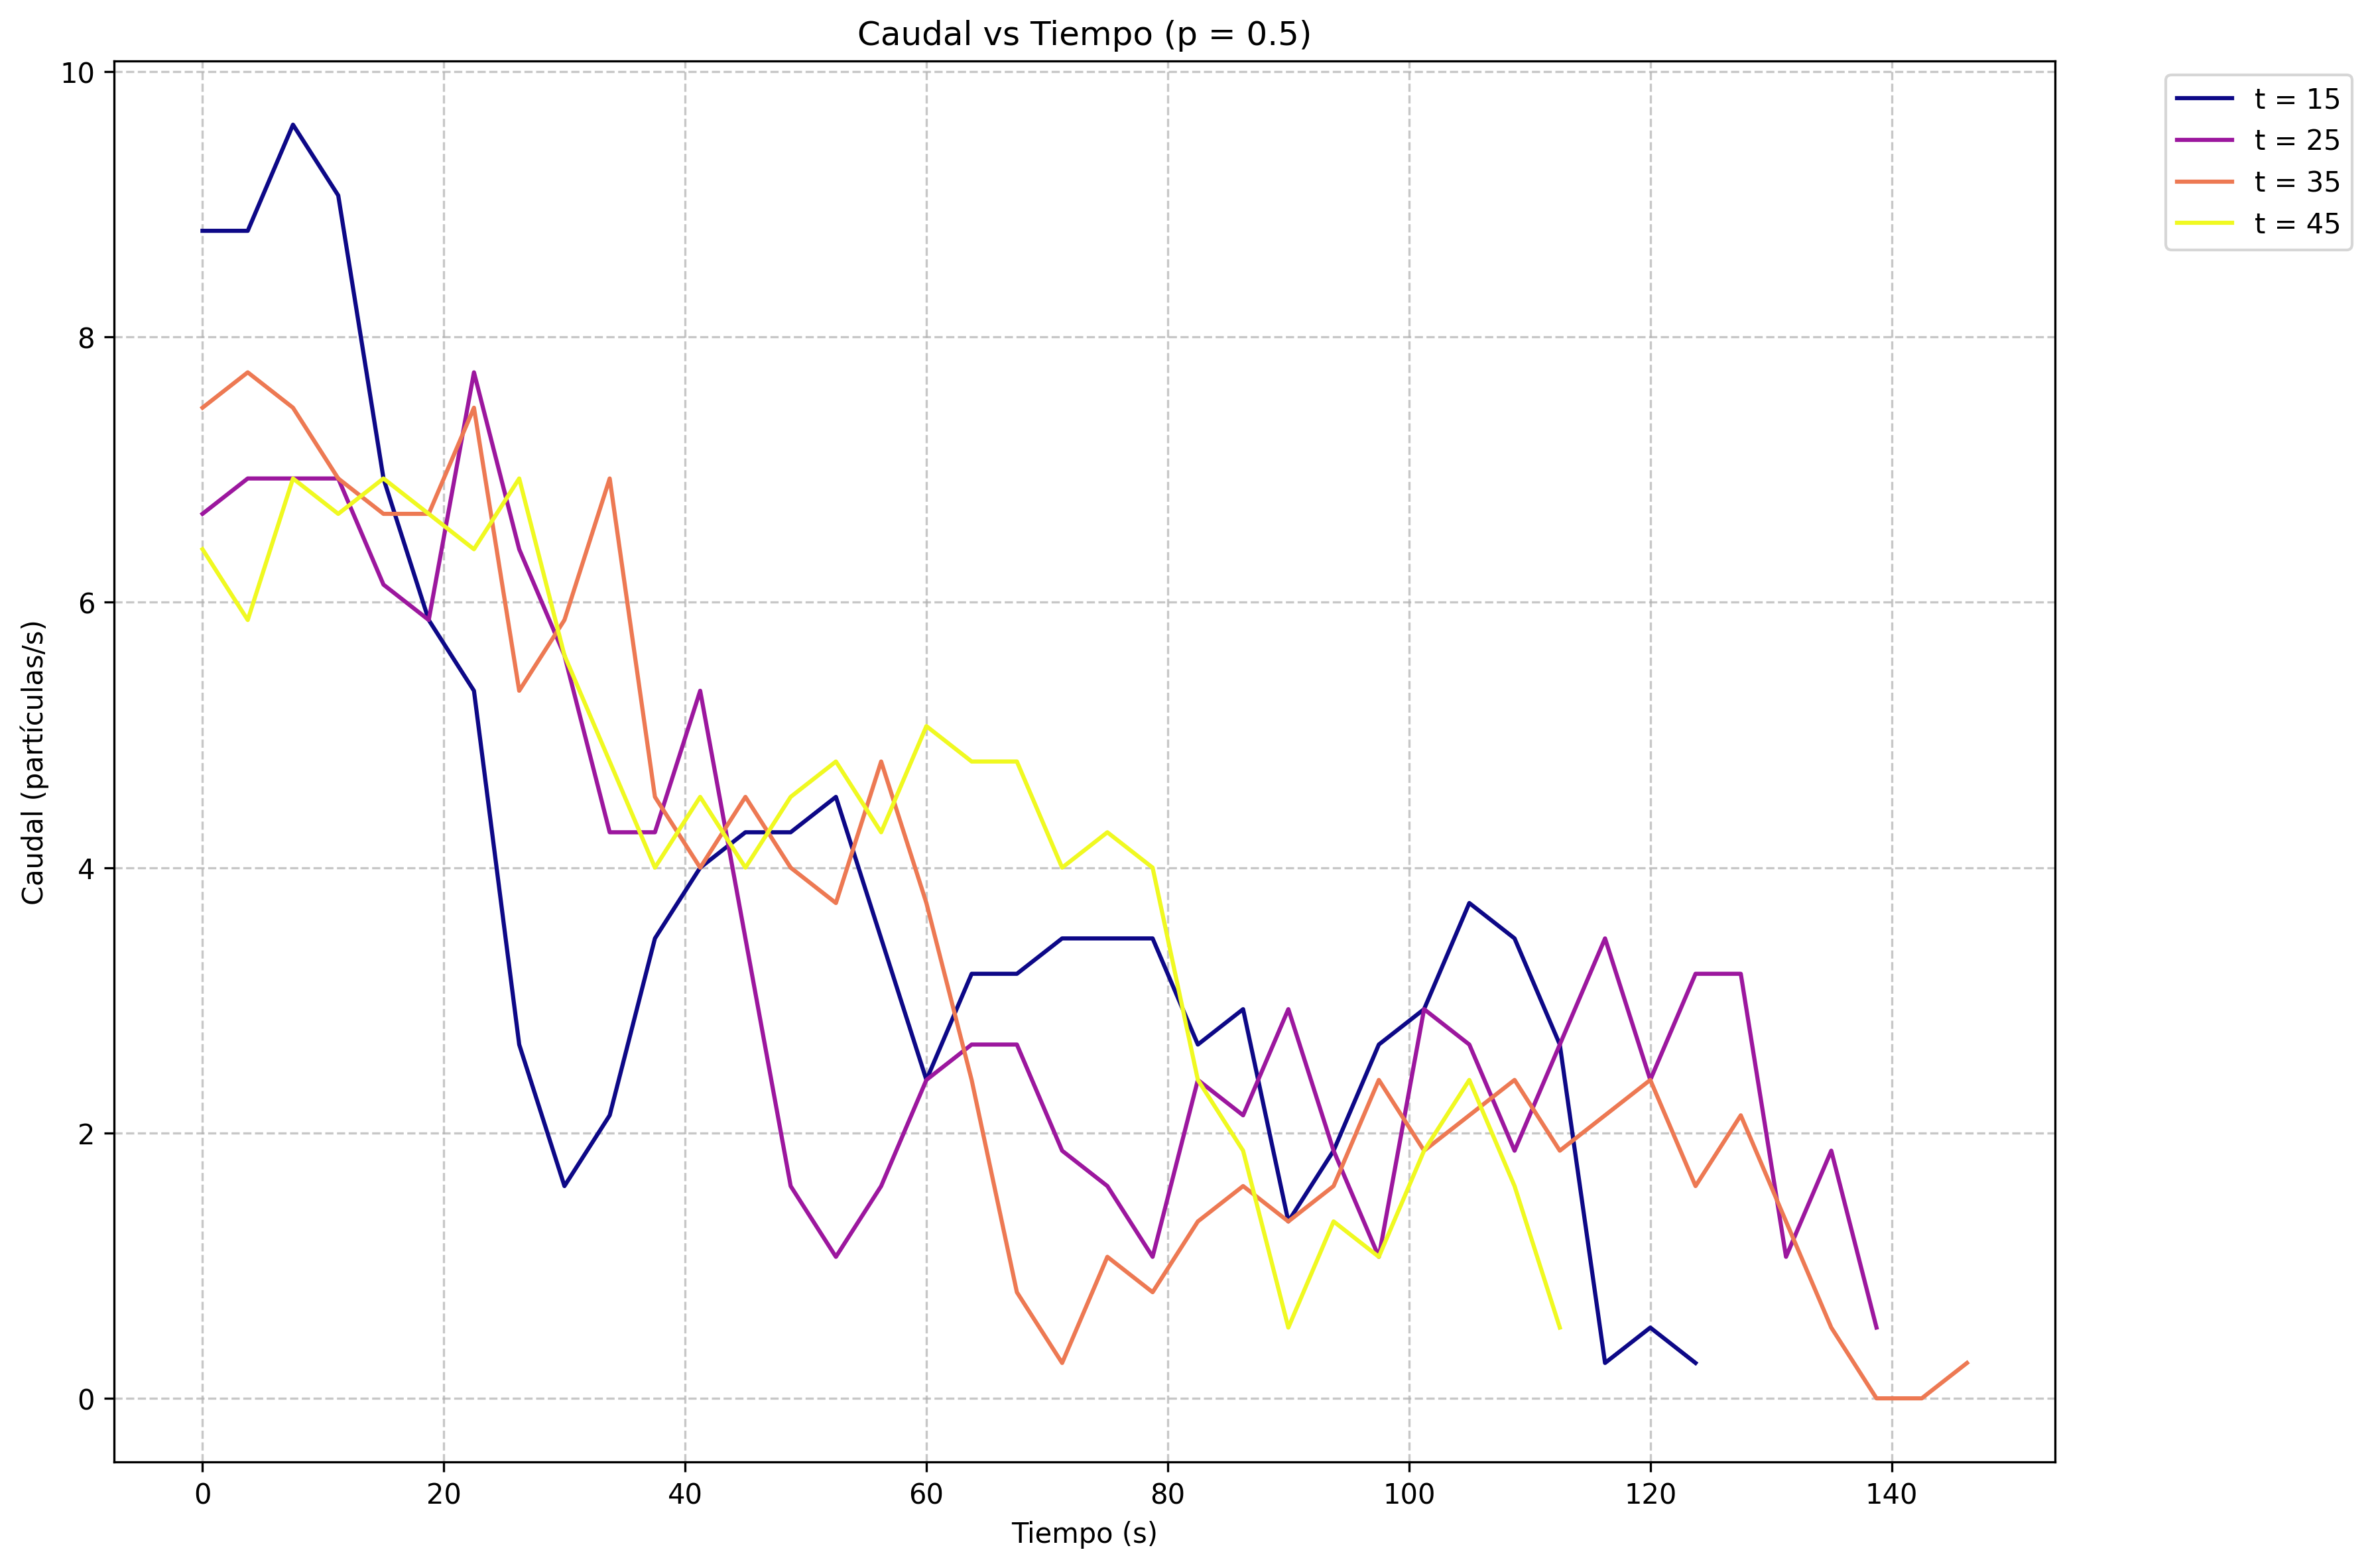
\includegraphics[width=0.6\textwidth]{img/flow_rates_p0.5.png}
        \caption{Caudal global en función del tiempo para $p=0.5$}
        \label{fig:flow_p100}
    \end{figure}    
\end{frame}

\begin{frame}{Densidad en función de $ct$}
    \begin{figure}[H]
        \centering
        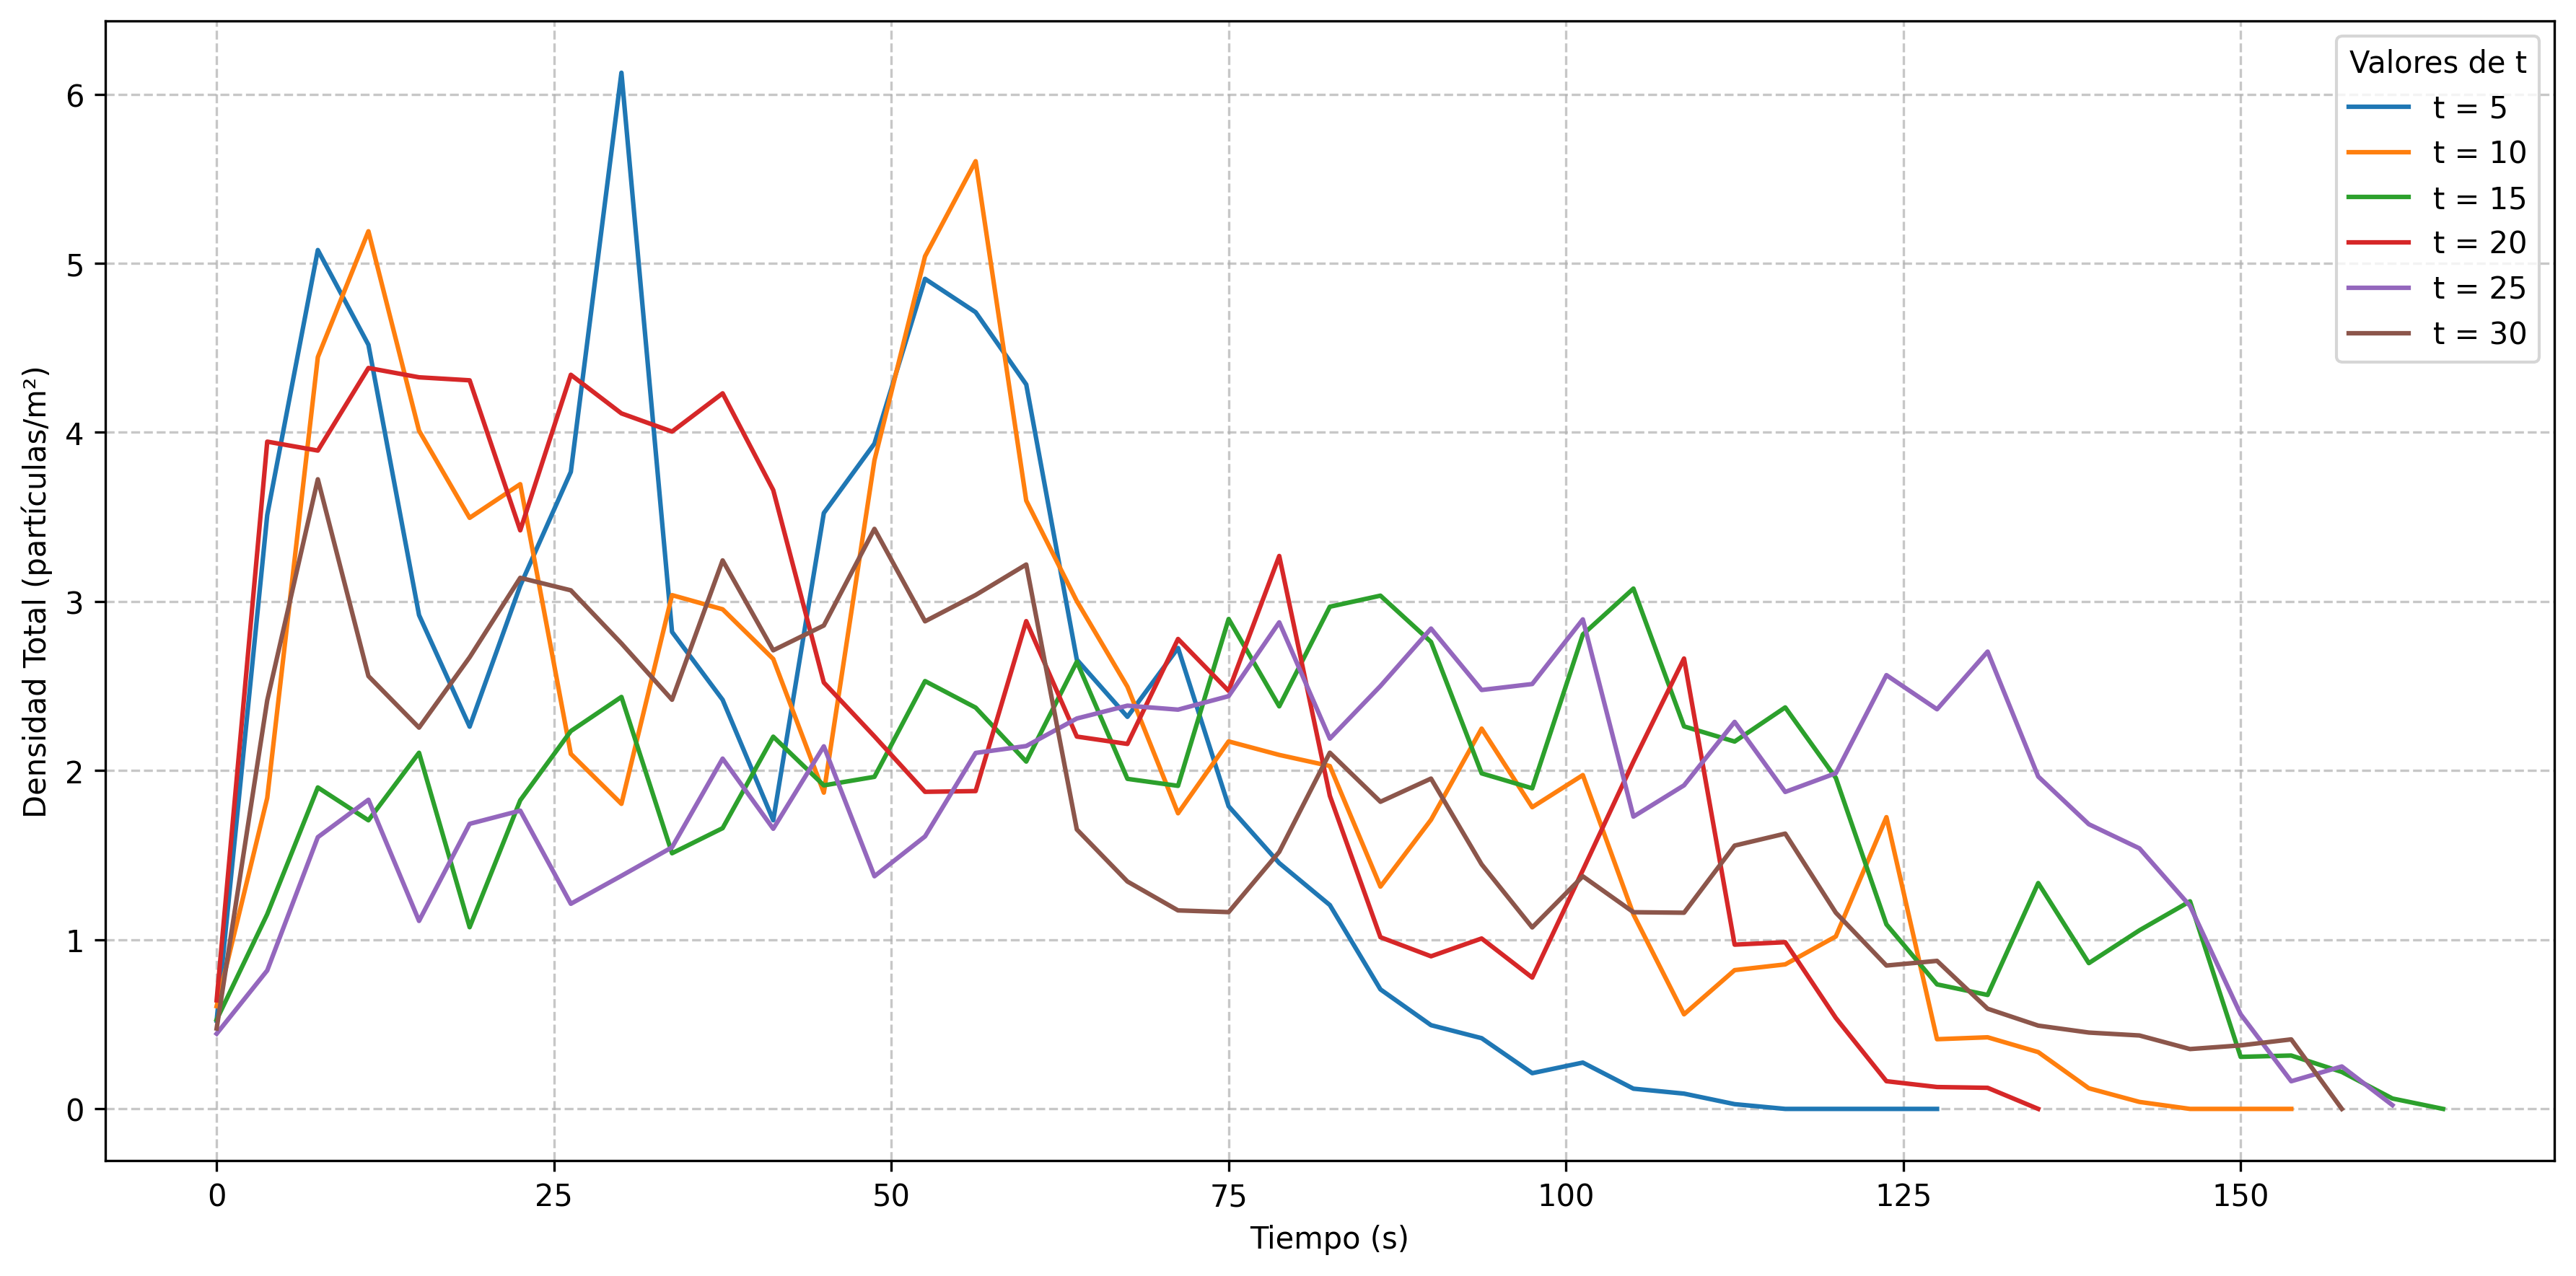
\includegraphics[width=0.6\textwidth]{img/density_vs_time_p0.50.png}
        \caption{Densidad en función del tiempo para $p=0,5$}
        \label{fig:flow_p100}
    \end{figure}    
\end{frame}

\begin{frame}{Densidad media en función de $ct$}
    \begin{figure}[H]
        \centering
        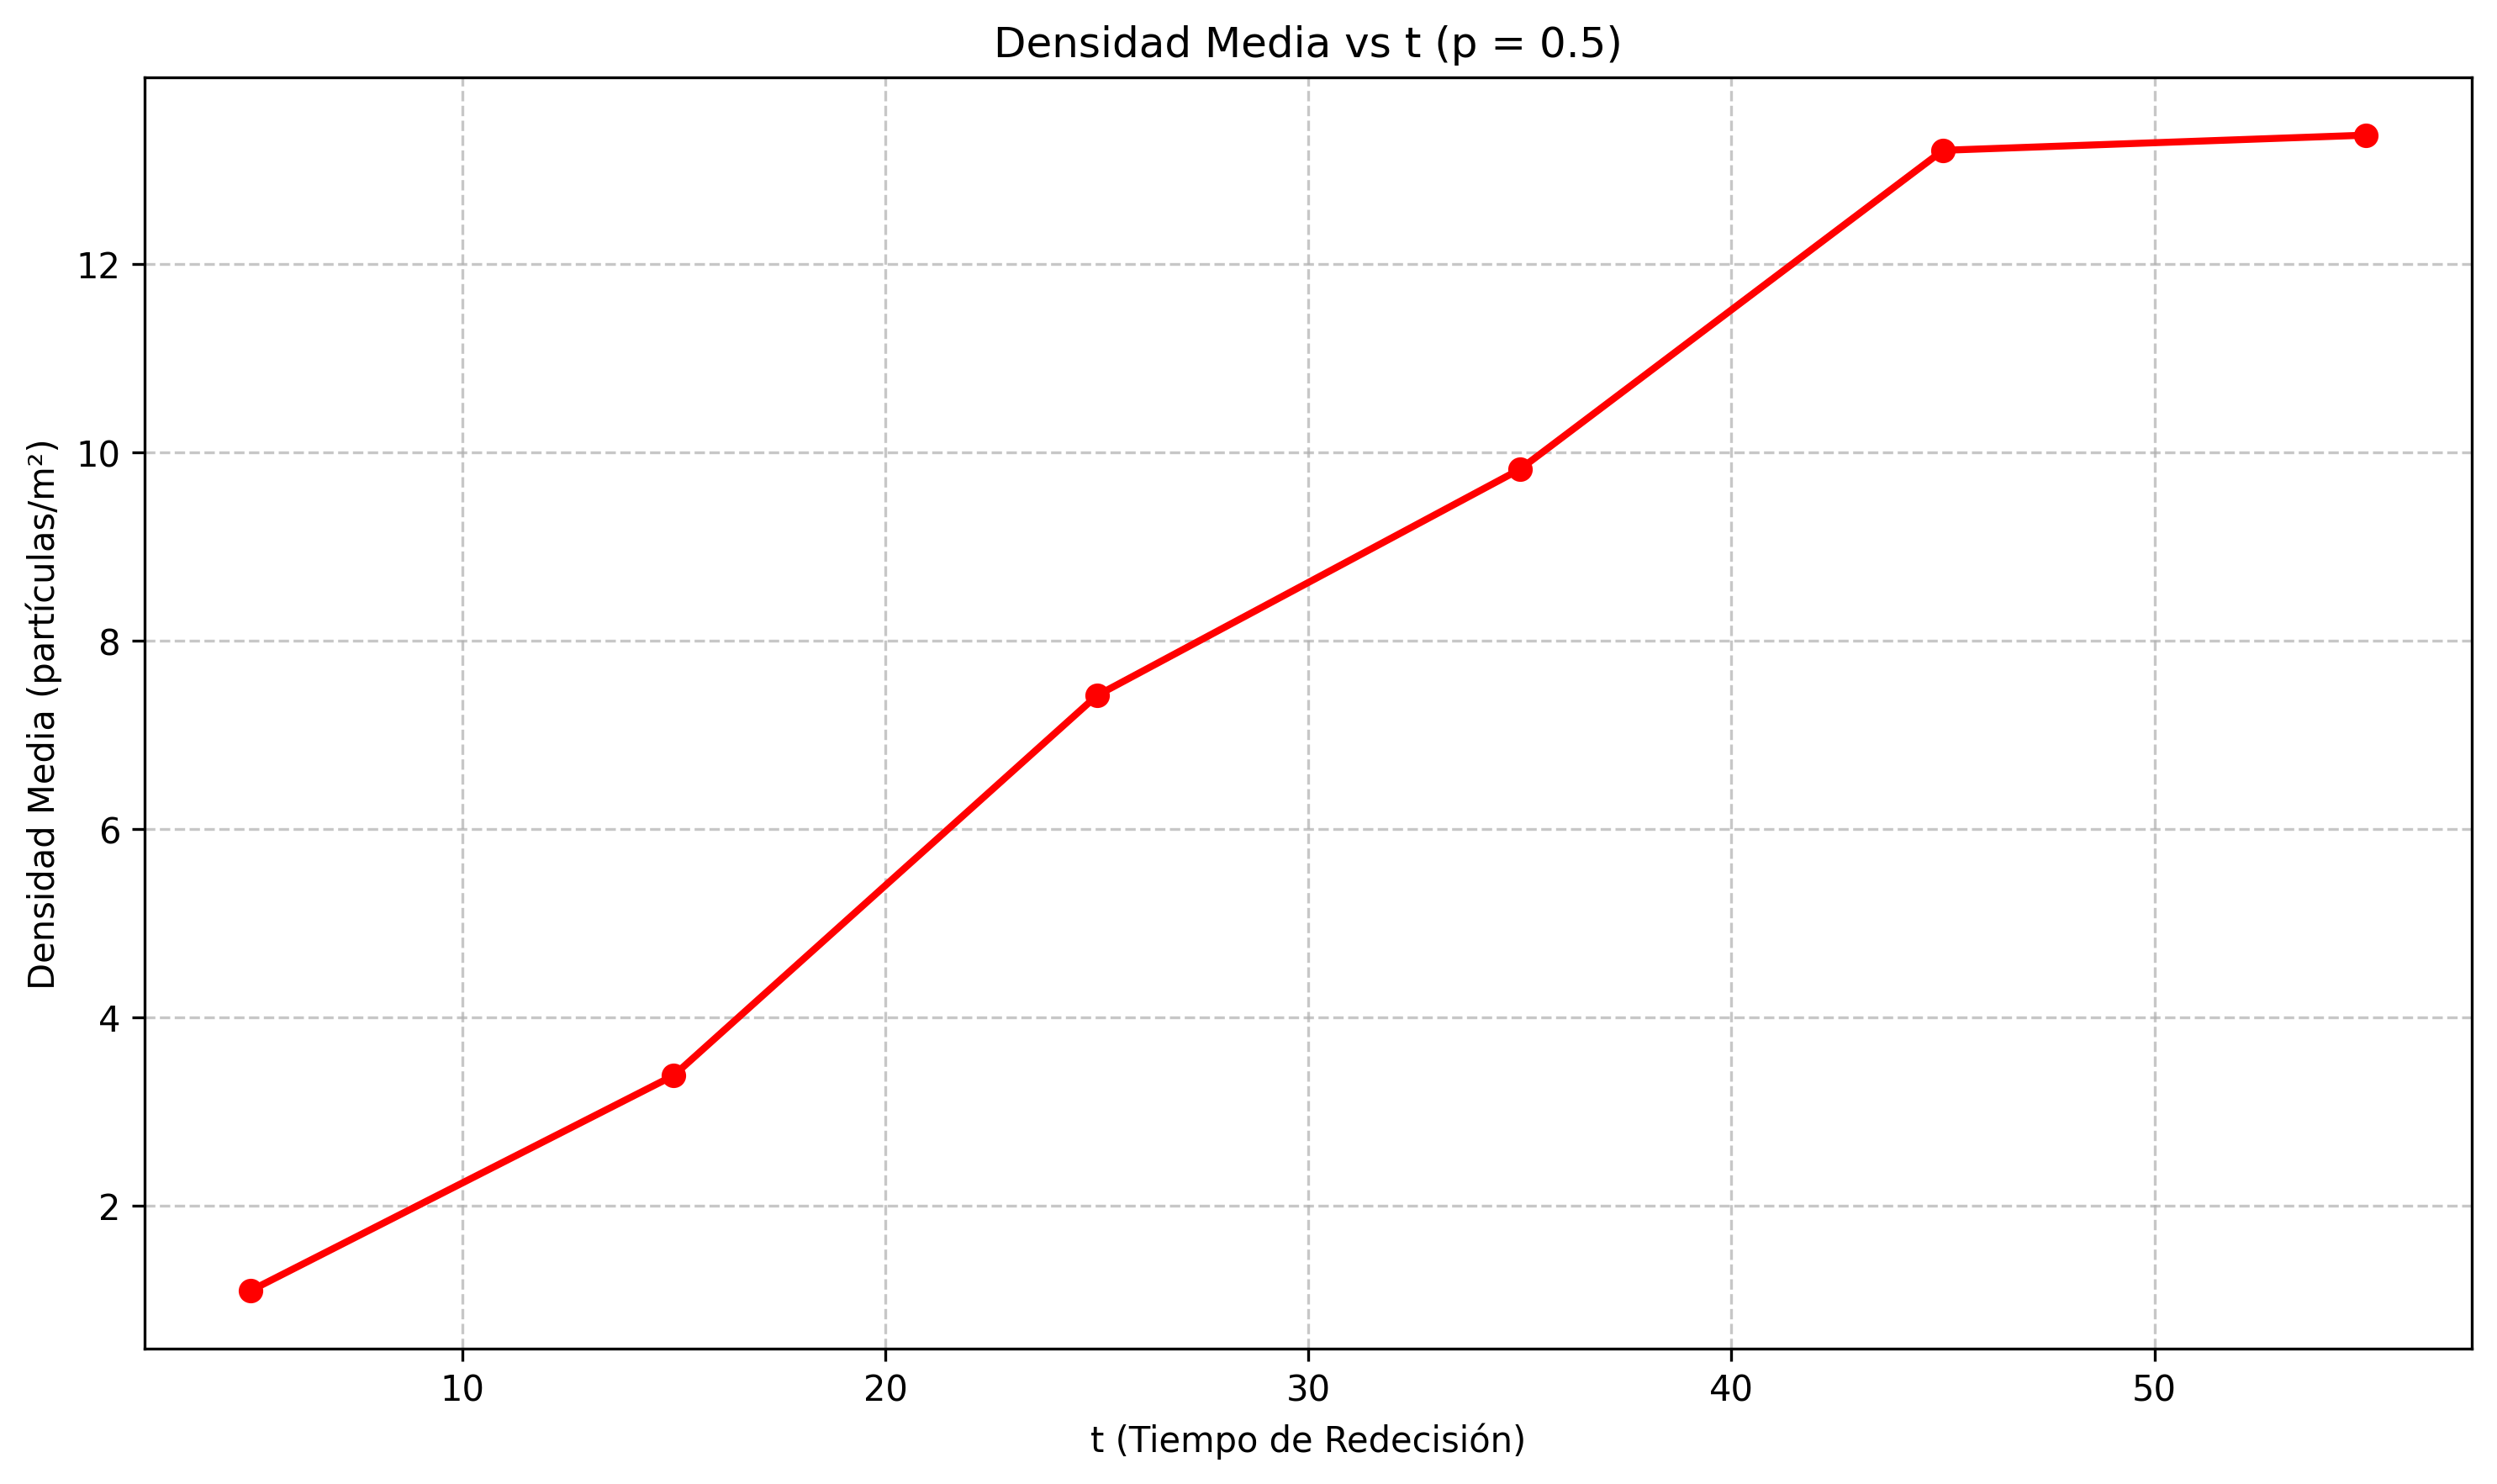
\includegraphics[width=0.6\textwidth]{img/average_density_p0.50.png}
        \caption{Densidad media en función de $ct$ para $p=0,5$}
        \label{fig:flow_p100}
    \end{figure}    
\end{frame}


\begin{frame}{Coeficiente de uniformidad en función de $ct$}
    \begin{figure}[H]
        \centering
        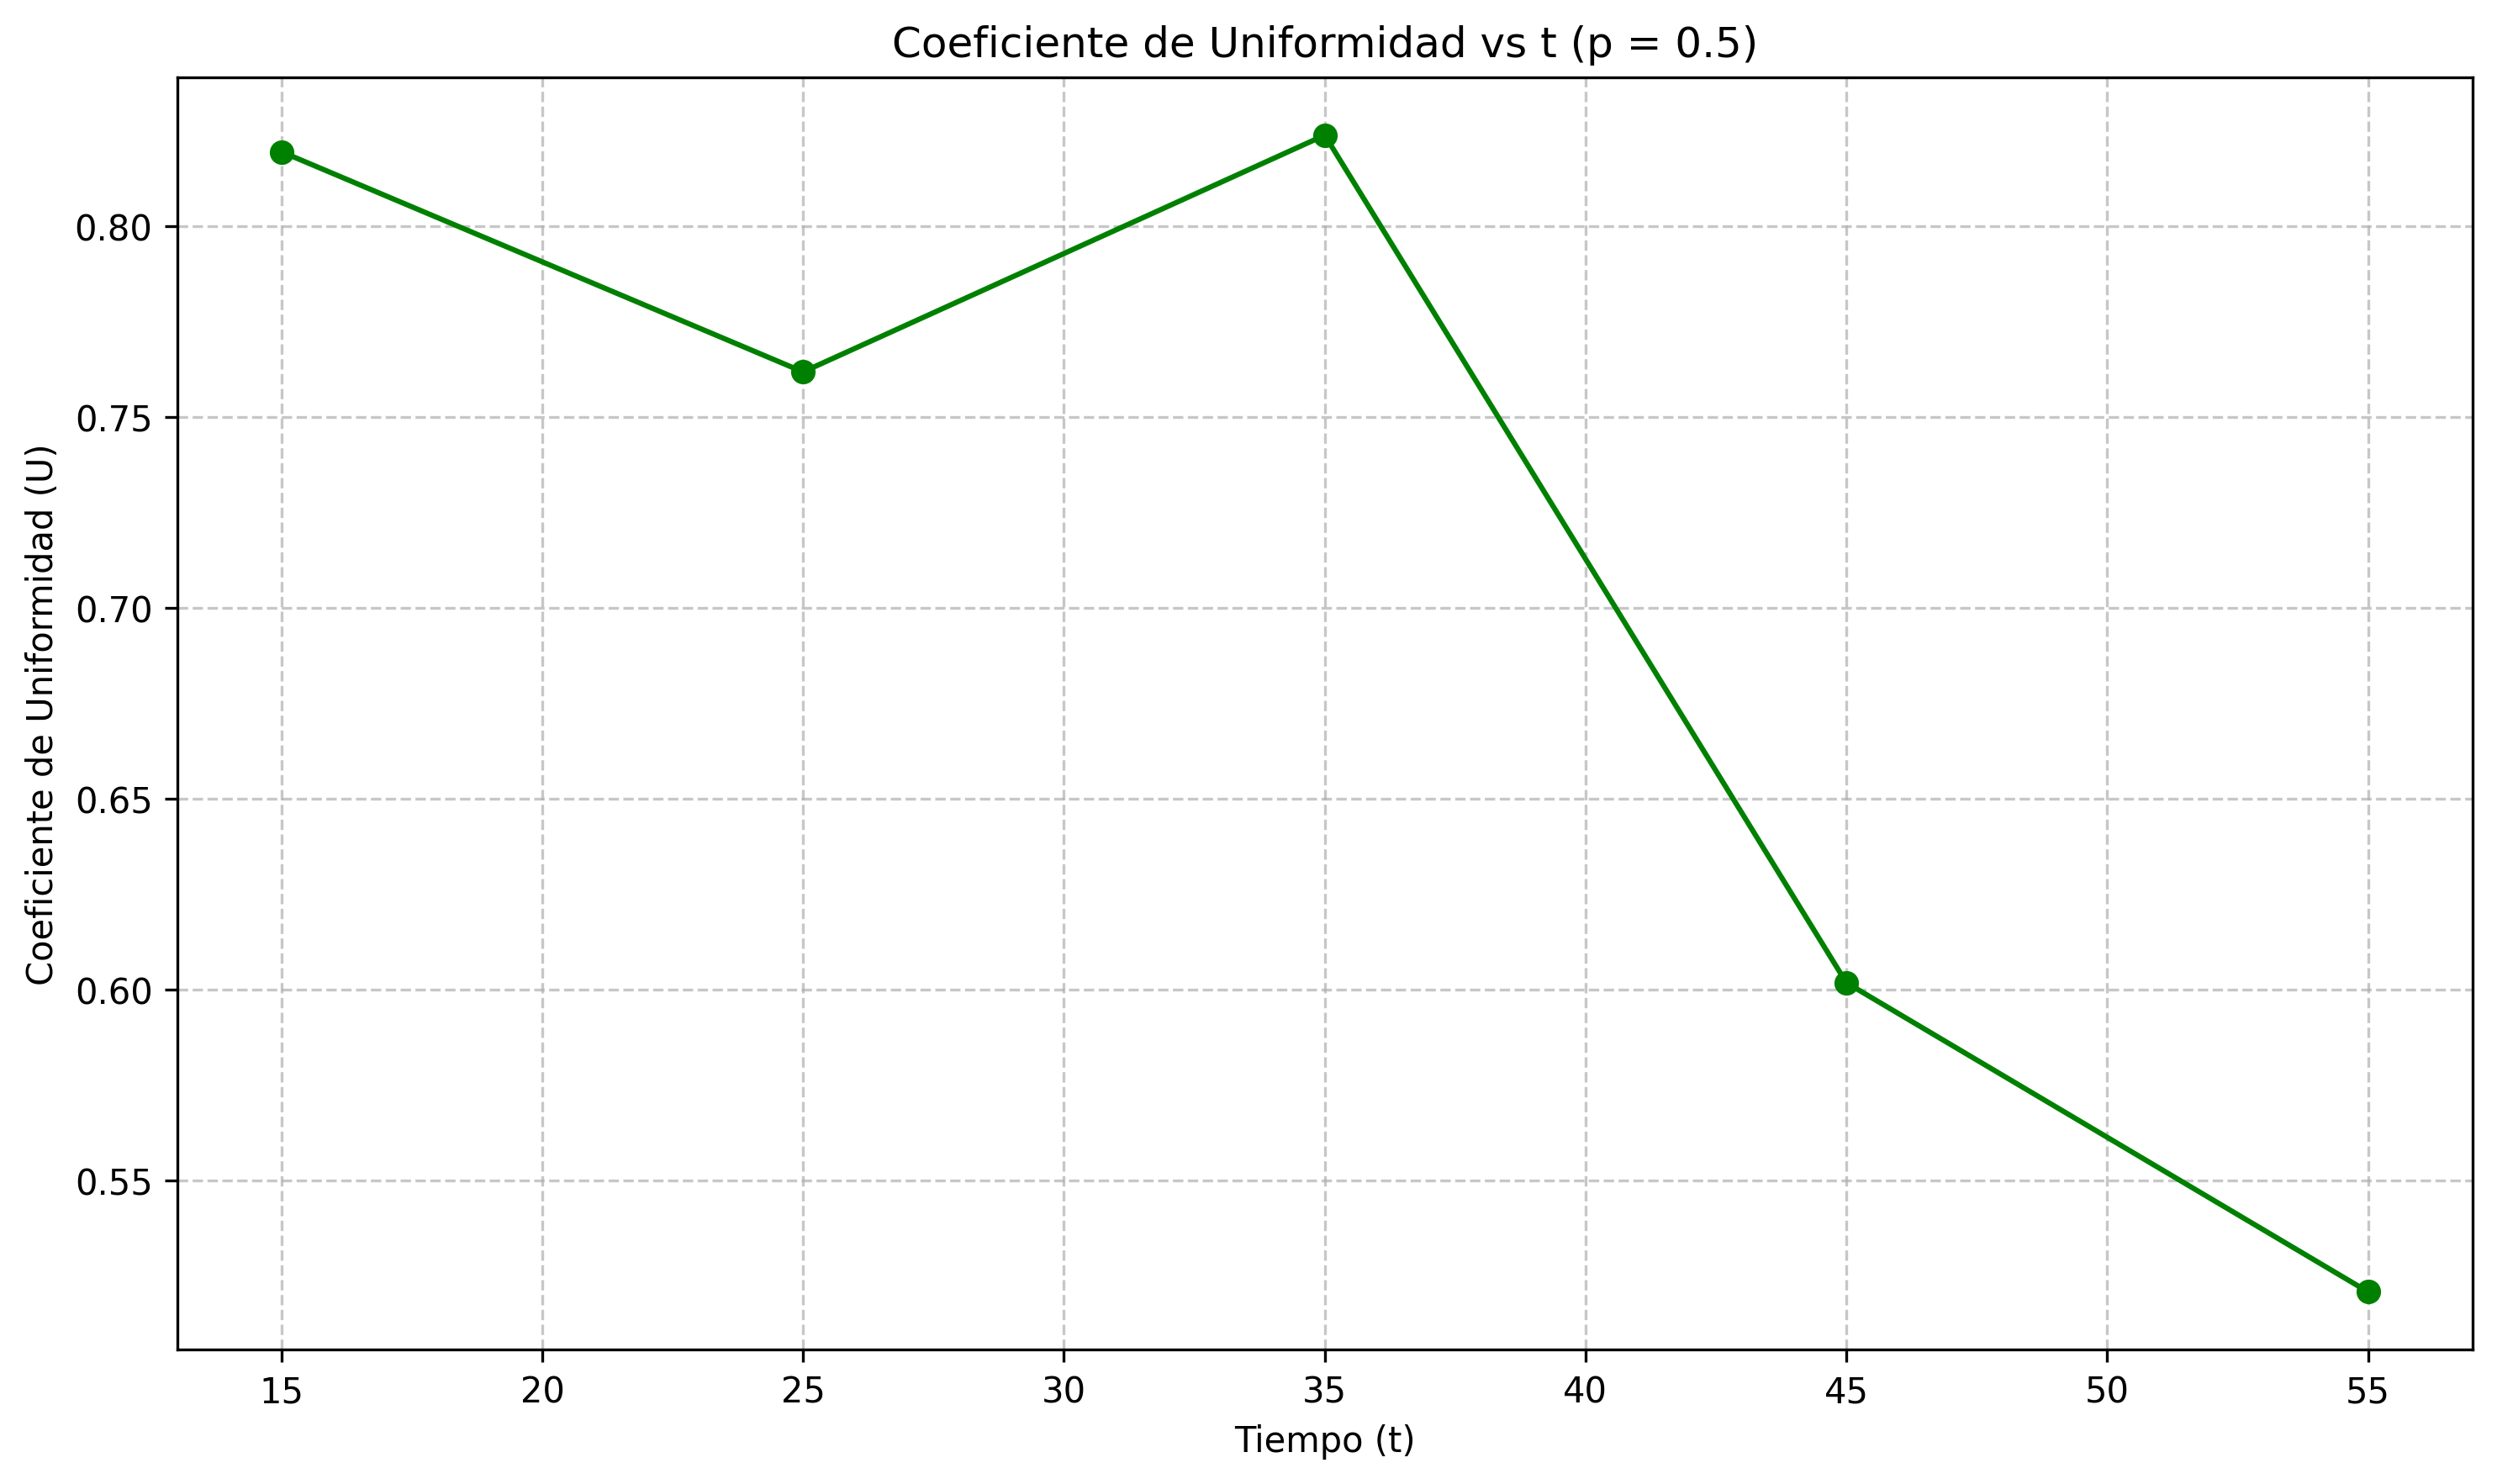
\includegraphics[width=0.6\textwidth]{img/uniformity_vs_t_p0.5.png}
        \caption{Coeficiente de uniformidad para $p=0,5$}
        \label{fig:flow_p100}
    \end{figure}    
\end{frame}


\section{Conclusiones}

\begin{frame}{Conclusiones}
    \begin{itemize}
        \item La priorización de distancia ($p=1.00$):
        \begin{itemize}
            \item Evacuaciones más rápidas
            \item Mayor congestión en salidas cercanas
        \end{itemize}
        \item Balance distancia-densidad ($p=0.50$):
        \begin{itemize}
            \item Distribución más uniforme del flujo
            \item Tiempo de evacuación moderado
        \end{itemize}
        \item Priorización de densidad ($p=0.00$):
        \begin{itemize}
            \item Evacuaciones más lentas
            \item Menor congestión en salidas
        \end{itemize}
    \end{itemize}
\end{frame}

\end{document}